
\documentclass{article}

\usepackage{amsfonts}
\usepackage{listings}
\usepackage{amsmath}
\usepackage{amssymb}
\usepackage{caption}
\usepackage{changepage}
\usepackage[italian]{babel}
\usepackage[letterpaper,top=2cm,bottom=2cm,left=2cm,right=2cm,marginparwidth=1.75cm]{geometry}
\usepackage{mathtools} 
\usepackage{forest}

\usepackage{pgfplots}
\usepackage{graphicx}
\usepackage{svg}
\usepackage{array}
\usepackage{pgfplots}
\usepackage{tikz}
%\usepackage[outputdir=build]{minted}
\usepackage[outputdir=build]{minted}

\usepackage{tikz} 
\usetikzlibrary{trees}
\usepackage{siunitx}
\usepackage{tablefootnote}
\usepackage{threeparttable}
\usepackage{pgfplots}
\usepgfplotslibrary{groupplots}

\usepackage[utf8]{inputenc}
\usepackage[colorlinks=true, allcolors=blue]{hyperref}
\pgfplotsset{compat=newest}
\usetikzlibrary{arrows.meta, positioning, patterns}
\usepgfplotslibrary{fillbetween}
\usetikzlibrary{arrows.meta, positioning, shapes.geometric, calc}
\usetikzlibrary{arrows,positioning,shapes.geometric}
\pgfplotsset{compat=newest}
\usetikzlibrary{positioning, arrows.meta, fit, calc, shapes}

\title{Appunti di sistemi di comunicazione}
\author{Leonardo Giovannoni}

\begin{document}
\maketitle
\section*{Introduction}


le comunicazioni wireless rappresentano la quota più importante in termini di utenti oggigiorno. Lo spettro delle comunicazioni radio risulto molto affollato, soprattutto nella banda dell'ordine dei GHz in cui si trovano molteplici applicazioni.

\begin{table}[h!]
\centering
\begin{tabular}{ | m{2cm} | m{3cm} | m{2.5cm} | m{4cm} | m{2.5cm} | }
\hline
Banda di frequenza & Intervallo di frequenza & Lunghezza d'onda & Servizi & Propagazione \\
\hline
LF & 30 -- 300 kHz & \(10^{4} - 10^{3}\) m & Orologio radio, navigazione (LORAN), militare (marina) & Onda di terra \\
\hline
MF & 0.3 -- 3 MHz & \(10^{3} - 10^{2}\) m & Radio AM (522--1600 kHz), radiofari & Onda di terra, onda ionosferica \\
\hline
HF & 3 -- 30 MHz & \(10^{2} - 10\) m & Comunicazioni aeronautiche, radar oltre l'orizzonte, radioamatori & Onda ionosferica \\
\hline
VHF & 30 -- 300 MHz & \(10 - 1\) m & Comunicazioni avioniche, radio FM (88 -- 108 MHz), DVB-T (RAI \(177.5\) MHz) & Onda spaziale \\
\hline
UHF & 0.3 -- 3 GHz & \(1 - 10^{-1}\) m & DVB-T (470-860 MHz), Cellulare (\(900,1800,2200\) MHz), Wi-Fi, GPS & Onda spaziale \\
\hline
SHF & 3 -- 30 GHz & \(10^{-1} - 10^{-2}\) m & Wi-Fi, 5G, DVB-S, Radar, SatCom & Onda spaziale \\
\hline
EHF & 30 -- 300 GHz & \(10^{-2} - 10^{-3}\) m & Wi-Fi, 5G, DVB-S, Radar, SatCom & Onda spaziale \\
\hline
\end{tabular}
\end{table}

\begin{itemize}
    \item \textbf{LF (Low Frequency)}: Frequenze molto basse, utilizzate per orologi radio, sistemi di navigazione a lunga distanza come LORAN, e comunicazioni militari navali. La propagazione è principalmente per onda di terra.
    \item \textbf{MF (Medium Frequency)}: Queste frequenze includono la banda di trasmissione AM. Sono utilizzate anche per i radiofari. Le onde possono viaggiare come onde di terra o riflettersi nell'ionosfera (onde ionosferiche).
    \item \textbf{HF (High Frequency)}: Utilizzate per comunicazioni aeronautiche, radar a lungo raggio e dai radioamatori. Queste onde si propagano principalmente attraverso l'ionosfera.
    \item \textbf{VHF (Very High Frequency)}: Coprono servizi come le comunicazioni avioniche e le trasmissioni radio FM. La propagazione è principalmente diretta, conosciuta anche come onda spaziale o visuale.
    \item \textbf{UHF (Ultra High Frequency)}: Include servizi come la televisione digitale terrestre (DVB-T), comunicazioni cellulari, Wi-Fi e GPS. La propagazione è di tipo spaziale, e queste onde richiedono generalmente una linea di vista libera tra trasmettitore e ricevitore.
    \item \textbf{SHF (Super High Frequency) e EHF (Extremely High Frequency)}: Utilizzate per servizi avanzati come il Wi-Fi, il 5G, le trasmissioni satellitari (DVB-S), i radar e le comunicazioni satellitari (SatCom). Anche queste si propagano attraverso onda spaziale o visuale.
\end{itemize}

Incrementando la frequenza di ha una banda di trasmissione maggiore, tuttavia la distanza di trasmissione diminuisce.

\begin{itemize}
    \item \textbf{Onde di terra}: Hanno una bassa frequenza e si propagano vicino alla superficie terrestre. Sono utilizzate per comunicazioni a lunga distanza.
    \item \textbf{Onde ionosferiche}: Hanno una frequenza media, sono riflesse dalla ionosfera e possono viaggiare a lunghe distanze.
    \item \textbf{Onde spaziali}: Hanno una frequenza elevata e si propagano in linea retta. Richiedono una linea di vista libera tra trasmettitore e ricevitore.
\end{itemize}

La questione dell'occupazione della banda è un argomento molto trattato attualmente in quanto trasmissioni alla solita frequnza generano collisioni non promuovendo la ricostruzione del segnale trasmesso. Per ridurre le collisioni si utilizzano tecniche di modulazione e codifica del segnale.



\section*{Comunicazioni analogiche}

Amplitude Modulation Double Side Band (AM-DSB) è generalmente utilizzata per trasmettere solo la voce.
Il segnale \( s_{DSB}(t) \) è definito come:

\begin{equation*}
    s_{DSB}(t) = A_c m(t) \cos(2\pi f_c t)
\end{equation*}

\begin{center}
    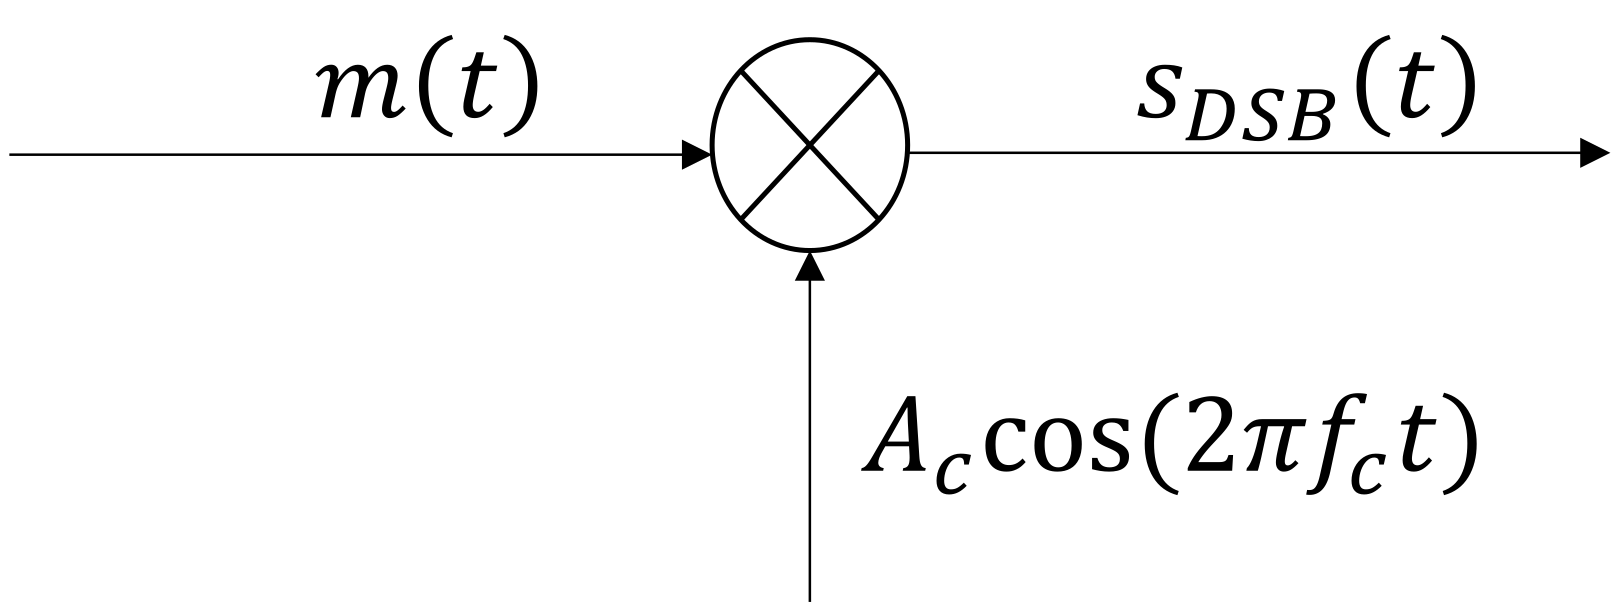
\includegraphics[width=0.25\textwidth]{imgs/analog_pam_trasmitter.png}
\end{center}
dove:
\begin{itemize}
    \item \( m(t) \) è il segnale modulante, o il messaggio.
    \item \( A_c \) è l'ampiezza del segnale portante.
    \item \( \cos(2\pi f_c t) \) è l'onda portante alla frequenza \( f_c \).
\end{itemize}

\begin{center}
    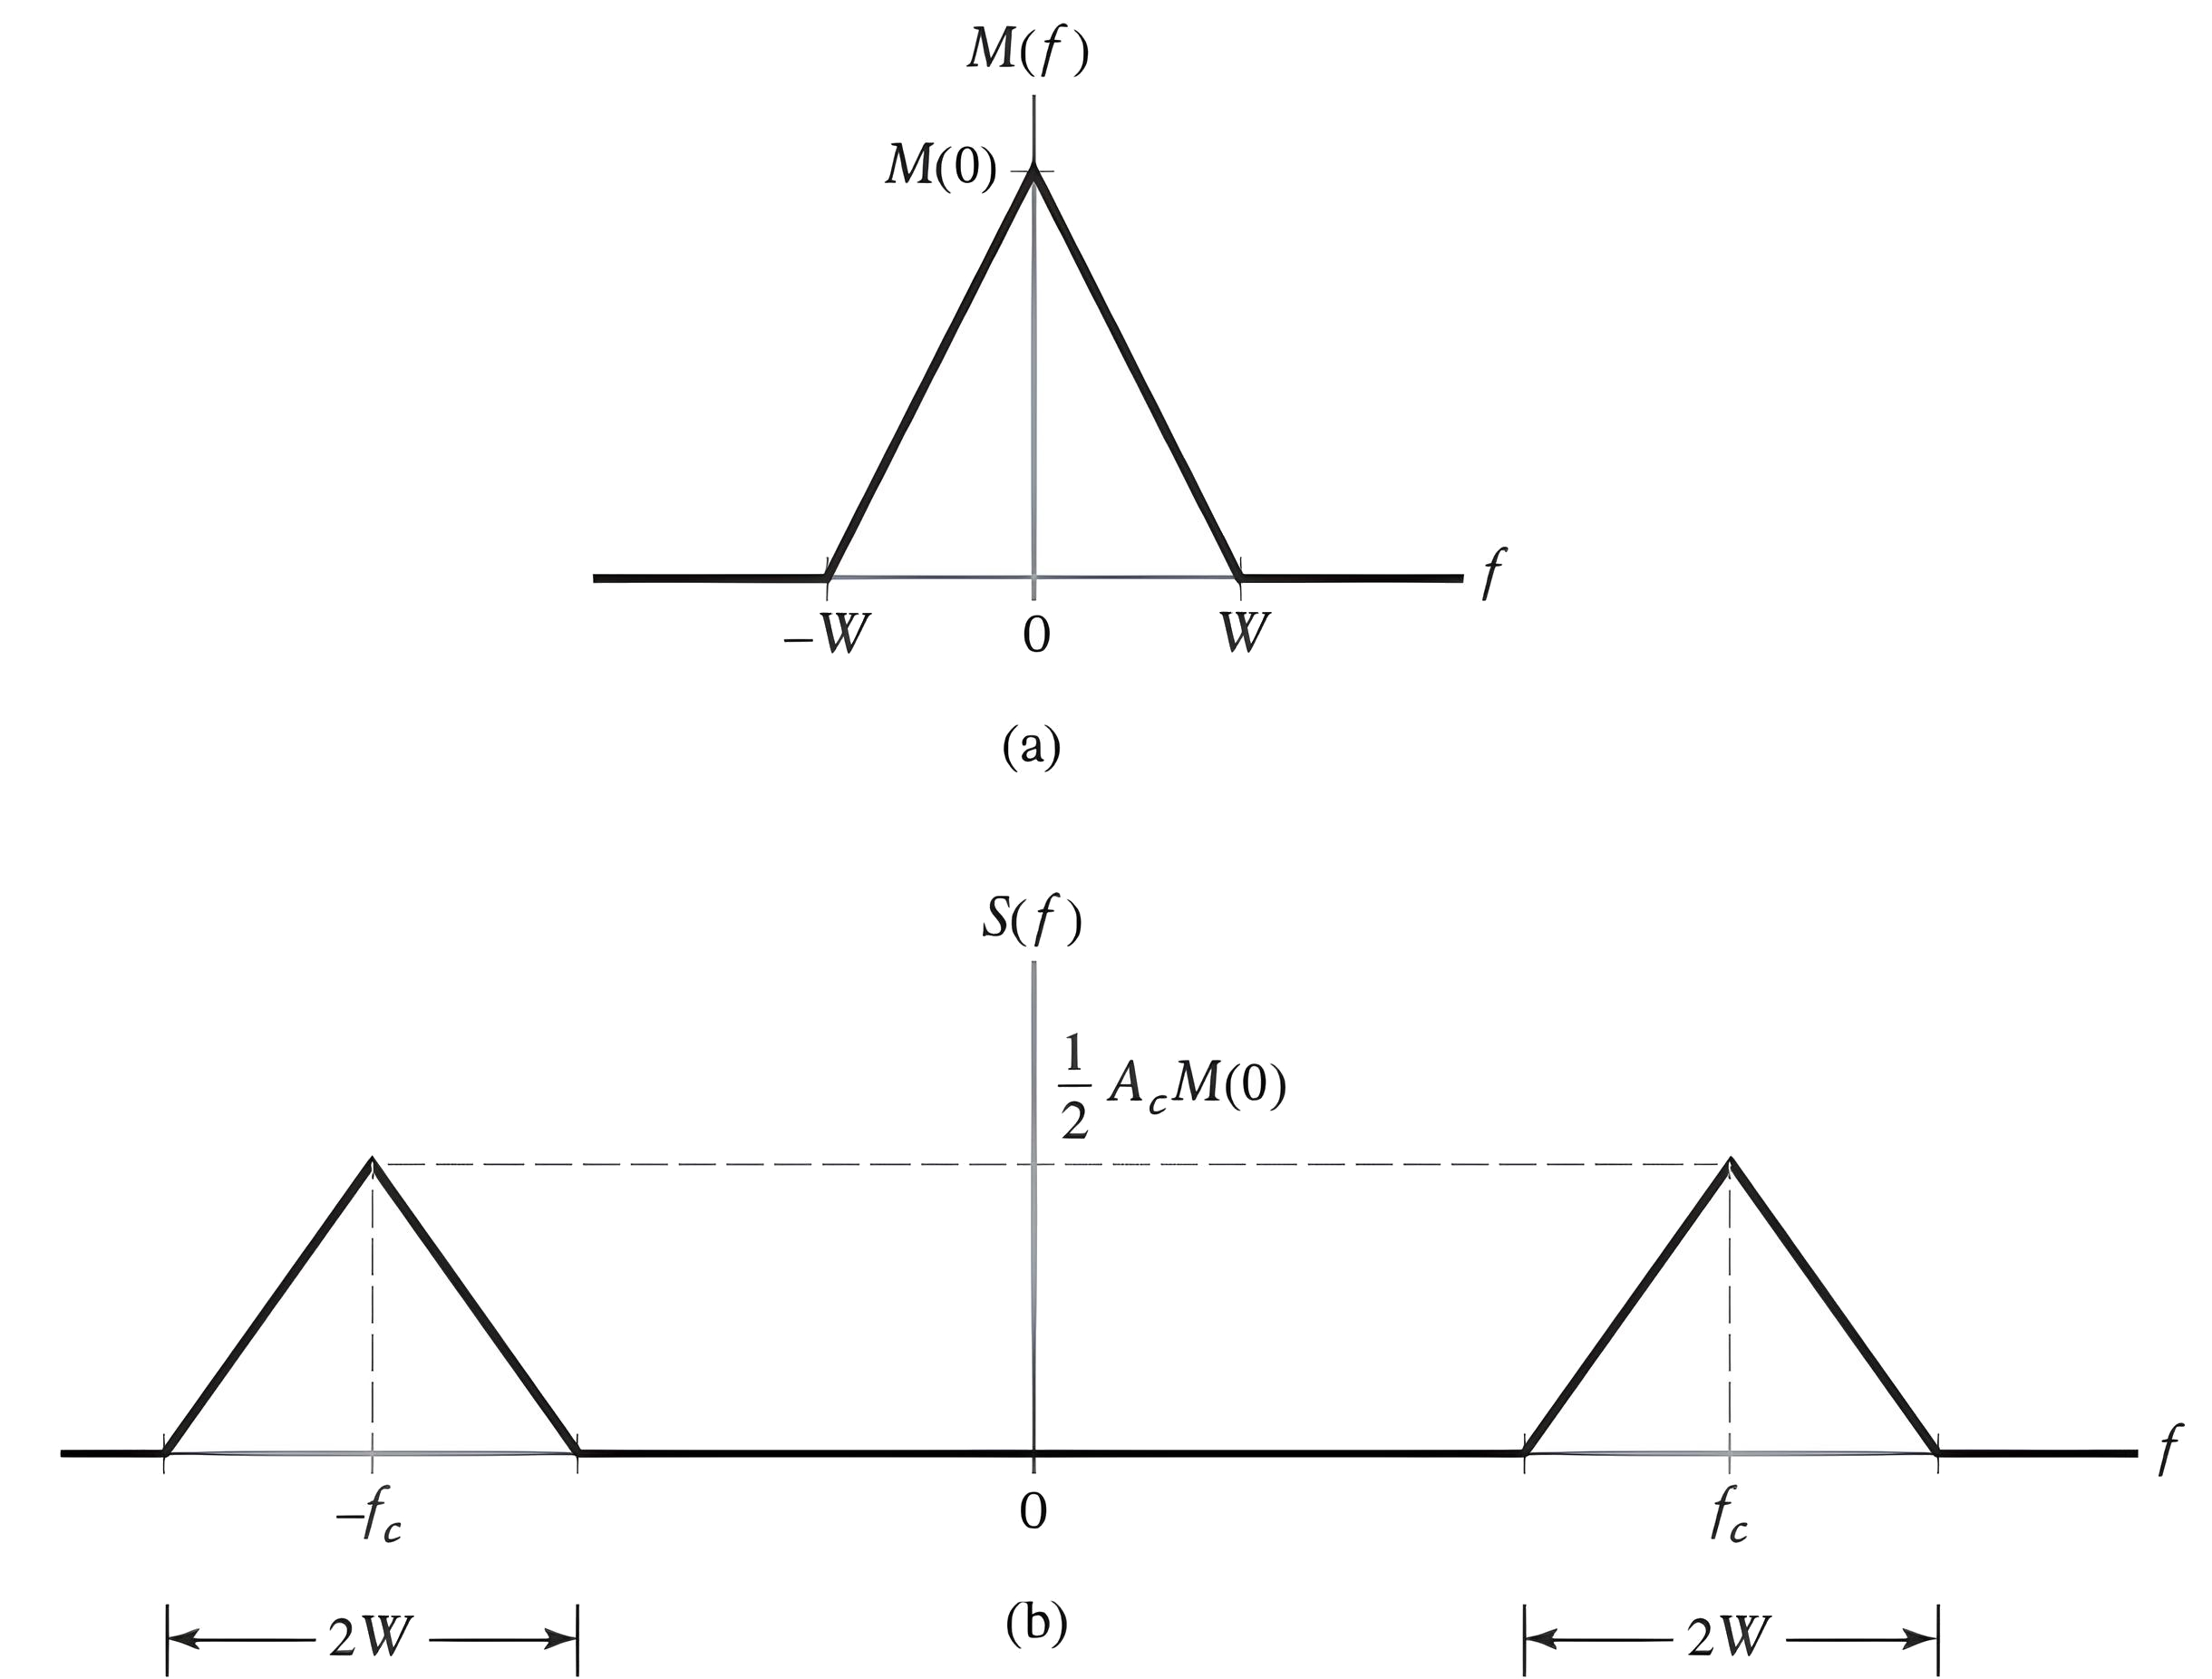
\includegraphics[width=0.5\textwidth]{imgs/dsb.jpg}
\end{center}


La modulazione AM-DSB è caratterizzata da due bande laterali, ciascuna localizzata tra \( f_c \pm W \) e \( -f_c \pm W \), dove \( W \) è la banda del segnale modulante. Queste bande laterali trasportano la stessa informazione, da cui il termine \textbf{dual sideband}.

Effettuando la trasformata di Fourier\footnote{$X(f) \triangleq \int_{-\infty}^{+\infty} x(t) e^{-j2\pi ft} dt$} di \( s_{DSB}(t) \), otteniamo la rappresentazione nel dominio delle frequenze \( s_{DSB}(f) \). Ciò è calcolabile come segue:
\[
    s_{DSB}(f) = A_c \ \mathcal{F}\{m(t)\} (f)  \ast \mathcal{F}\{\cos(2\pi f_c t) \}(f) = A_c M(f) \ast \frac{\delta(f - f_c) + \delta(f + f_c)}{2} =
\]

\[
    = \frac{1}{2} A_c [M(f - f_c) + M(f + f_c)]
\]
Sebbene la componente negativa possa essere trascurata adesso la traslazione del segnale alla frequenza $f_c \gg W$ comporta un'occupazione di banda di $2W$ per ogni lato, ma ciò comporta uno spreco in quanto si ha duplicazione di informazione.

\begin{center}
    \tikzsetnextfilename{am}
    \documentclass{standalone}

\usepackage{tikz,pgf} %and any other packages or tikzlibraries your picture needs

\begin{document}



\begin{tikzpicture}
    \begin{axis}[
        title={AM-DSB Modulation},
        xlabel={Time},
        ylabel={Amplitude},
        axis lines=middle,
        ymax=2,
        ymin=-2,
        xtick=\empty,
        ytick=\empty,
        clip=false,
        no markers,
        width=10cm,
        height=5cm
    ]
    \addplot [domain=0:2*pi, samples=100, name path=m] {sin(deg(x))};
    \addlegendentry{$m(t)$}

    \addplot [domain=0:2*pi, samples=100, name path=carrier] {1.5*cos(deg(5*x))};
    \addlegendentry{$A_c \cos(2\pi f_c t)$}

    \addplot [domain=0:2*pi, samples=100, red, name path=am] {1.5*sin(deg(x))*cos(deg(5*x))};
    \addlegendentry{$s_{DSB}(t)$}

    \addplot [domain=0:2*pi, samples=100, dashed, name path=upper] {1.5*sin(deg(x))};
    \addplot [domain=0:2*pi, samples=100, dashed, name path=lower] {-1.5*sin(deg(x))};

    \addplot[fill=gray!30] fill between[of=upper and lower];

    \end{axis}
\end{tikzpicture}
\end{document}

\end{center}


Il segnale \( s_{DSB}(t) \) dopo essere stato filtrato dal filtro passa-banda (BPF) conserva la sua forma.
La demodulazione è implementata moltiplicando \( s_{DSB}(t) \) con una portante sincronizzata \( 2\cos(2\pi f_c t) \).
Questo comporta la presenza di una componente ad alta frequenza a \( 2f_c \) che viene rimossa dal filtro passa-basso (LPF), lasciando solo il segnale messaggio \( m(t) \).
\begin{center}
    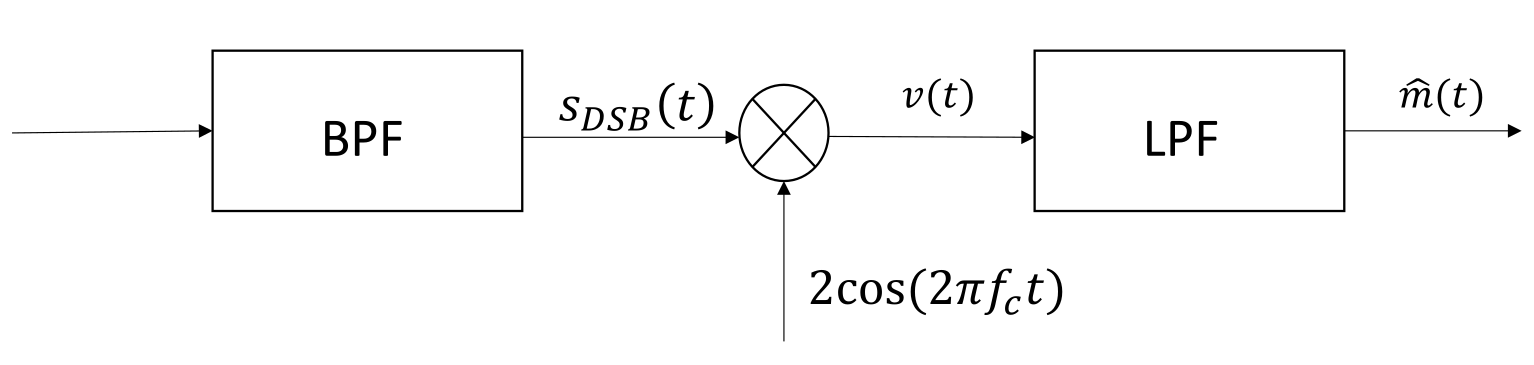
\includegraphics[width=0.625\textwidth]{imgs/analog_pam_receiver.png}
\end{center}

Dopo la demodulazione e il filtraggio, lo spettro è centrato nuovamente in banda base, recuperando il segnale messaggio.

Definiamo $B = 2W$.
Nella radio AM si ha una carrier frequency tra i 500 e i 1600 kHz e una $W$ tra i 5 e i 10 kHz.
Il segnale è pari (in modulo) a causa della simmetria hermitiana, infatti essendo $m(t)$ reale, $M(-f) = M^*(f)$ e quindi $|M(-f)| = |M(f)|$.


La ricostruzione del segnale originario richiede tre step:
\begin{itemize}
    \item \textbf{Filtraggio passa-banda}: il segnale ricevuto è filtrato tramite un filtro passa-banda, centrato in \( f_c \), per rimuovere le componenti fuori banda.
    \item \textbf{Demodulazione}: il segnale modulato viene moltiplicato per un secondo coseno, ottenendo oltre al segnale originario anche due contributi in \(\pm 2f_c \)
    \item \textbf{Filtraggio passa-basso}: il segnale demodulato viene filtrato con un filtro passa basso di ampiezza W, per rimuovere la componente ad alta frequenza.
\end{itemize}

\begin{equation*}
    v(t) = s_{DSB}(t) \cdot 2\cos(2\pi f_c t) = A_c m(t) \cdot 2\cos^2(2\pi f_c t) = A_c m(t) + A_c m(t) \cos(4\pi f_c t)
\end{equation*}

L'ipotesi $f_c^{(t)} = f_c^{(r)}$ garantisce la possibilità di effettuare il passaggio trigonometrico e dunque ricostruire il segnale originario senza alcuna distorsione. Tuttavia a prescindere dalla bontà dell'oscillatore utilizzato non è possibile ottenere una sincronizzazione perfetta senza alcuna logica aggiuntiva, un reale sistema di modulazione AM prevede tale meccanismo.

\section*{Analog Quadrature Amplitude Modulation}

\begin{center}
    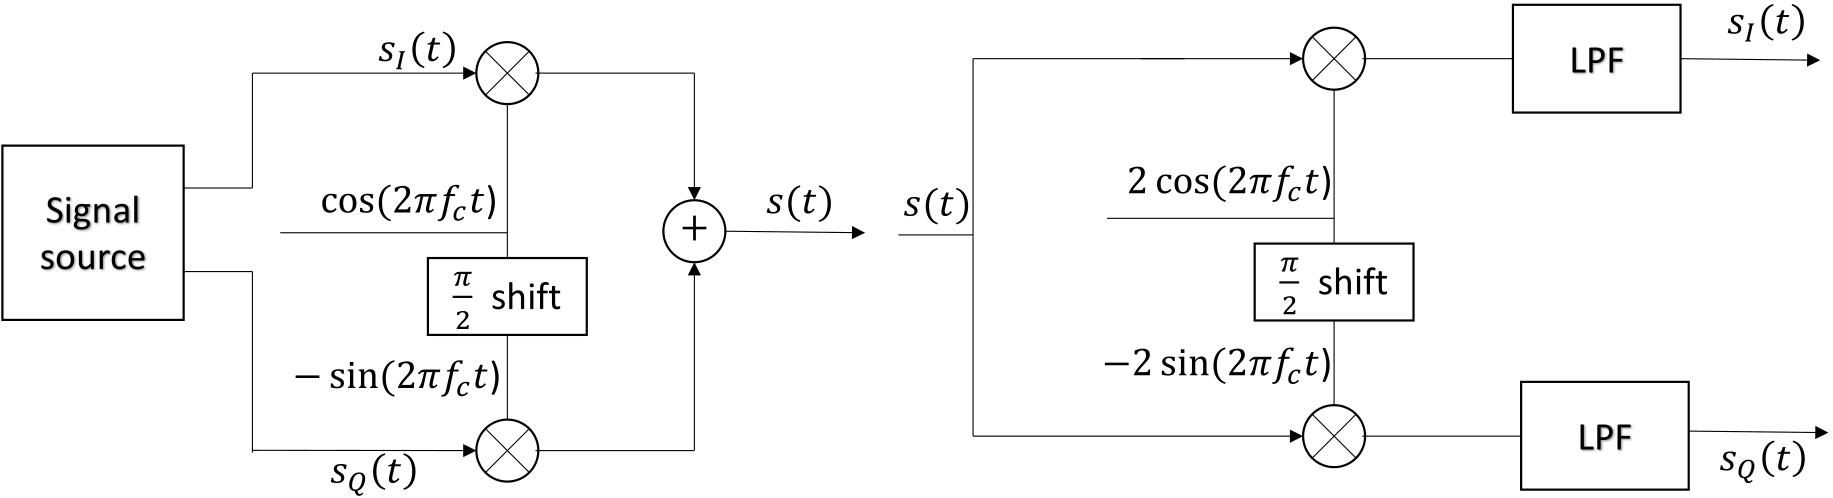
\includegraphics[width=1\textwidth]{imgs/analog_qam.png}
\end{center}

Per raddoppiare la quantità di informazioni trasmesse all'interno della stessa banda si può sfruttare l'ortogonalità della funzione seno e coseno, in modo da trasmettere contemporaneamente due segnali, occupando in modo ottimale la banda a disposizione. Tale modulazione è detta QAM, il termine quadrature indica lo shift di $\pi/2$ tra le due funzioni portanti (seno e coseno), mentre amplitude ricorda che si tratta comunique di una modulazione in cui l'informazione è trasportata interamente dall'ampiezza del segnale. L'ampiezza del segnale portante è infatti modulata in modo proporzionale all'ampiezza del segnale modulante, contente l'informazione da trasmettere.


Il segnale composto QAM \( s(t) \) può essere rappresentato come la somma di due segnali modulati DSB, uno modulato con un coseno (la componente in fase) e l'altro con un seno (la componente in quadratura):
\begin{equation}
    s_{QAM}(t) = A_{c} m_1(t) \cos(2\pi f_c t) - A_{c} m_2(t) \sin(2\pi f_c t)
\end{equation}

Dove:
\begin{itemize}
    \item \( m_1(t) \) e \( m_2(t) \) sono i segnali che contengono il messaggio per le componenti in fase e in quadratura, rispettivamente.
    \item \( f_c \) è la frequenza della portante.
\end{itemize}


La demodulazione del segnale QAM è effettuata moltiplicando il segnale composto \( s(t) \) con \( 2\cos(2\pi f_c t) \) e \( -2\sin(2\pi f_c t) \) per ottenere le componenti in fase \( s_I(t) \) e in quadratura \( s_Q(t) \), rispettivamente.
Questi prodotti sono poi filtrati con filtri passa-basso per estrarre i segnali contenenti il messaggio originali \( m_1(t) \) e \( m_2(t) \).
La demodulazione è fatta nella seguente maniera:
\begin{equation}
    v_I(t) = s(t) \cdot 2\cos(2\pi f_c t) = A_{c} m_1(t) + A_{c} m_1(t) \cos(4\pi f_c t) - A_{c} m_2(t) \sin(4\pi f_c t)
\end{equation}
\begin{equation}
    v_Q(t) = s(t) \cdot (-2\sin(2\pi f_c t)) = A_{c} m_2(t) - A_{c} m_1(t) \cos(4\pi f_c t) - A_{c} m_2(t) \sin(4\pi f_c t)
\end{equation}

Le componenti ad alta frequenza sono filtrate dal filtro passa-basso, ottenendo così i segnali originali \( m_1(t) \) e \( m_2(t) \).
Lo spettro del segnale ottenuto tramite moduazione non risulta più simmetrico rispetto a $f_c$, tuttavia essendo un segnale reale resta valida la simmetria rispetto all'asse delle ordinate.
La mancanza di simmetria rispetto a $f_c$ implica la non esistenza di un segnale reale in grado di rappresentare lo spettro in banda base, in quanto verrebbe meno la simmetria rispetto alla frequenza 0.
Sebbene questa mancanza non precluda l'utilizzo della modulazione QAM, nella pratica risulta più semplice lo studio di un segnale in banda base.
\begin{itemize}
    \item La carrier frequency \( f_c \) non aggiunge informazione al segnale, ma viene utilizzata per traslare il segnale in frequenza.
    \item Il criterio di Nyquist richiede un campionamento ad una frequnza doppia rispetto alla banda del segnale, quindi nel caso di segnale passa-banda tale valore può essere molto elevato. Nel caso di segnale in banda base la frequenza di campionamento può essere nettamente inferiore.
\end{itemize}

Il criterio di Nyquist stabilisce che \( T \leq \frac{1}{2B} \), dove \( T \) è il periodo di campionamento e \( B \) è la banda del segnale, e quindi \( f_s \geq 2B \). Quindi nel nostro caso, $f_s \geq 2B$.
Un segnale è definito in passa banda quando la propria energia è concentrata all'interno di una banda $2W$ centrata attorno a una carrier frequency $f_c$, con il vincolo $f_c \gg W$.

\subsection*{Inviluppo Complesso di un Segnale in Banda Passante}
\begin{center}
    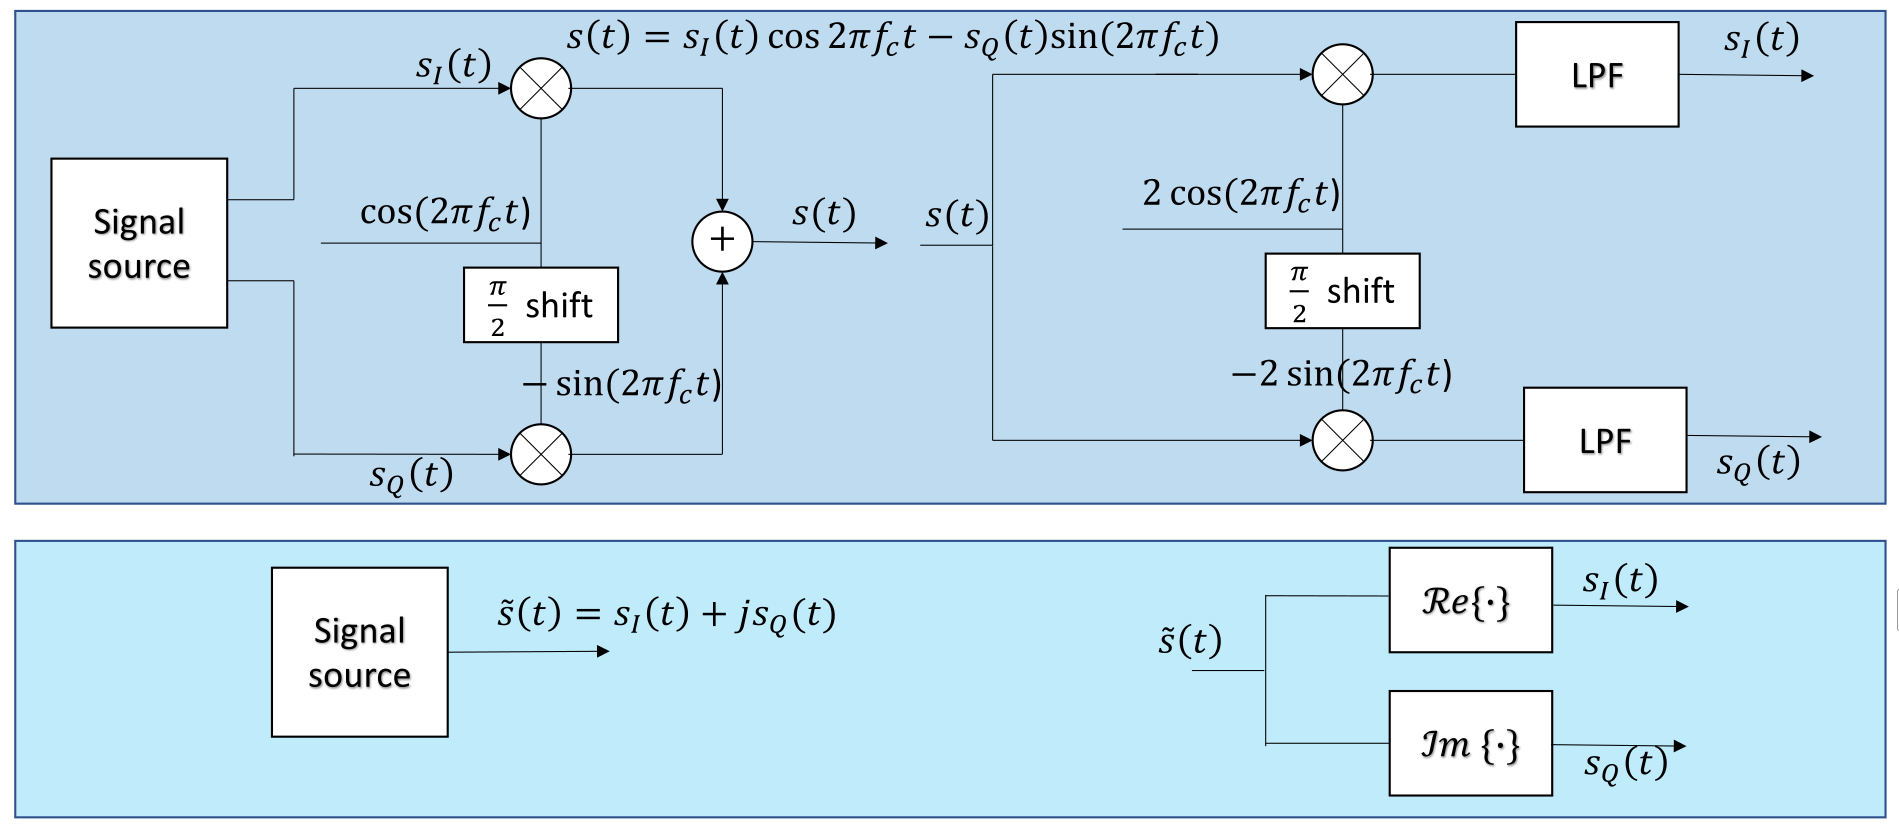
\includegraphics[width=1\textwidth]{imgs/complex_envelope.png}
\end{center}
La maggior parte dei sistemi di comunicazione opera in banda passante. Il segnale trasmesso \( s(t) \), concentrato in una banda di frequenza \( 2B \) e centrato attorno a una frequenza portante \( f_c \), risiede ben al di sopra della corrente continua (DC) o frequenza zero. Per un segnale in banda passante, vale la condizione \( f_c \gg 2B \), indicando che la frequenza portante è molto maggiore del doppio della larghezza di banda del segnale.

L'assenza di un segnale in banda base ha portato all'adozione dell'inviluppo complesso, definito come:
\begin{equation}
    \tilde{s}(t) = s_I(t) + js_Q(t) = A(t)e^{j\phi(t)}
\end{equation}
\begin{equation}
    s(t) = \Re\{\tilde{s}(t)e^{j2\pi f_c t}\} = s_I(t)\cos(2\pi f_c t) - s_Q(t)\sin(2\pi f_c t)
\end{equation}

Questo inviluppo complesso permette di rappresentare \( s(t) \) come la parte reale del prodotto del suo inviluppo complesso per un esponenziale complesso alla frequenza portante, facilitando l'analisi e la modulazione del segnale nei sistemi di comunicazione digitale. Per esempio, nella modulazione AM si ottiene:
\begin{equation}
    \tilde{s}_{AM}(t) = m(t) = A(t)e^{j\phi(t)}
\end{equation}
dove \( \phi(t) \) assume valore \( 0 \) o \( \pi \), essendo assente la componente immaginaria.

La sincronizzazione del clock tra trasmettitore e ricevitore è cruciale per una ricostruzione perfetta dell'informazione trasmessa, mantenendo la caratteristica di ortogonalità perfetta tra seno e coseno, necessaria per separare i due messaggi una volta modulati.

L'inviluppo complesso rappresenta un modello equivalente in banda base che facilita l'analisi e l'elaborazione dei segnali in banda passante come se fossero segnali in banda base, offrendo numerosi vantaggi:
\begin{itemize}
    \item Il modello in banda base è più semplice da studiare, poiché elimina gli effetti della frequenza portante dal modello del segnale, semplificando l'analisi matematica e la comprensione delle proprietà del segnale.
    \item La simulazione numerica di un modello in banda base richiede meno risorse computazionali rispetto a un modello in banda passante, grazie alla minor larghezza di banda necessaria.
    \item Di conseguenza, anche la frequenza di campionamento è inferiore per i modelli in banda base, il che si traduce in tassi di trasmissione dati ridotti, vantaggioso per l'elaborazione e lo stoccaggio del segnale digitale.
    \item Il modello in banda base è spesso la base per un'implementazione digitale di un sistema di comunicazione in banda passante, facilitando l'applicazione delle tecniche di elaborazione del segnale digitale, fondamentali nelle comunicazioni moderne.
\end{itemize}

\section*{Modulazione di Frequenza (FM)}

Nella modulazione di frequenza (FM), il messaggio è incorporato nella fase del segnale \( \phi(t) \). Il segnale FM \( s_{FM}(t) \) può essere espresso come:
\begin{equation}
    s_{FM}(t) = A_c \cos\left(2\pi f_c t + 2\pi k_f \int_{-\infty}^{t} m(\tau) d\tau \right)
\end{equation}

La fase \( \phi(t) \) del segnale FM è quindi data dall'integrale del segnale del messaggio \( m(t) \), scalato dalla sensibilità alla deviazione di frequenza \( k_f \):
\begin{equation}
    \phi(t) = 2\pi f_c t + 2\pi k_f \int_{-\infty}^{t} m(\tau) d\tau
\end{equation}

L'indice di modulazione \( m_f \) è definito come il rapporto tra la deviazione di frequenza e la larghezza di banda del messaggio \( f_m \):
\begin{equation}
    m_f = \frac{\Delta f}{f_m}
\end{equation}

%Δ𝑓 = max |𝑓7 (𝑡)| = 𝑘) max 𝑚(𝑡)
Dove $\Delta f = \max |f(t)| = k_f \max m(t)$.
La rappresentazione complessa del segnale FM può essere ottenuta utilizzando la formula di Eulero:
\begin{equation}
    s_{FM}(t) = \Re \left\{ A_c e^{j\phi(t)} \right\} = \Re \left\{ A_c e^{j2\pi f_c t} e^{j2\pi k_f \int_{-\infty}^{t} m(\tau) d\tau} \right\} = \Re \left\{ \tilde{s}_{FM} (t) e^{j2\pi f_c t} \right\}
\end{equation}

E quindi:
\begin{equation}
    \tilde{s}_{FM}(t) = A_c e^{j2\pi k_f \int_{-\infty}^{t} m(\tau) d\tau}
\end{equation}

Questa rappresentazione è particolarmente utile per l'analisi dei segnali FM nel contesto del trattamento digitale dei segnali.

I vantaggi della modulazione in frequenza includono:
\begin{itemize}
    \item Minore sensibilità ai disturbi, migliorando così la qualità del segnale ricevuto.
    \item Maggiore efficienza energetica, poiché il segnale informativo non richiede potenza aggiuntiva a quella della portante.
    \item L'ampiezza costante permette l'uso di amplificatori semplificati in fase di trasmissione, evitando la necessità di mantenere l'amplificatore nella zona lineare, come sarebbe necessario con le modulazioni di ampiezza variabile (AM).
    \item Possibilità di configurare la modulazione per ottimizzare il compromesso tra qualità della trasmissione e banda occupata.
\end{itemize}



\begin{center}
    \resizebox{0.5\textwidth}{!}{
        \tikzsetnextfilename{fm_waveform}
        \documentclass{standalone}

\usepackage{tikz,pgf} %and any other packages or tikzlibraries your picture needs

\usepackage{pgfplots}

\usepackage[utf8]{inputenc}
\usepackage[colorlinks=true, allcolors=blue]{hyperref}
\usetikzlibrary{positioning, arrows.meta, fit, shapes}
\begin{document}

  \begin{tikzpicture}[align=center]
            \begin{groupplot}[
                    group style={
                            group size=1 by 3,
                            vertical sep=1cm
                        },
                    width=14cm,
                    height=5cm
                ]

                \nextgroupplot[
                    xmin=0, xmax=12,
                    ymin=-1.5, ymax=1.5,
                    axis lines=middle,
                    xtick=\empty,
                    ytick=\empty,
                    xlabel={},
                    ylabel={},
                    title={Carrier ($f_c$)}
                ]
                \addplot[thick, domain=0:12, samples=200] {sin(deg(2*3.14*x))};
                \nextgroupplot[
                    xmin=0, xmax=12,
                    ymin=-1.5, ymax=1.5,
                    axis lines=middle,
                    xtick=\empty,
                    ytick=\empty,
                    xlabel={},
                    ylabel={},
                    title={Baseband Input ($f_m$)}
                ]
                \addplot[thick, domain=0:12, samples=200] {sin(deg(0.3*3.14*(x - 1.57)))};

                \draw[dashed] (axis cs:1.57,25) -- (axis cs:1.57,-25);
                \draw[dashed] (axis cs:3.235,25) -- (axis cs:3.235,-25);
                \draw[dashed] (axis cs:4.9,25) -- (axis cs:4.9,-25);
                \draw[dashed] (axis cs:6.565,25) -- (axis cs:6.565,-25);
                \draw[dashed] (axis cs:8.23,25) -- (axis cs:8.23,-25);
                \draw[dashed] (axis cs:9.895,25) -- (axis cs:9.895,-25);
                \draw[dashed] (axis cs:11.56,25) -- (axis cs:11.56,-25);

                \nextgroupplot[
                    xmin=0, xmax=12,
                    ymin=-2, ymax=1.5,
                    axis lines=middle,
                    xtick=\empty,
                    ytick=\empty,
                    xlabel={},
                    ylabel={},
                    title={FM waveform}
                ]
                \addplot[thick, domain=0:12, samples=200] {sin(deg(2*3.14*(x-0.5*sin(deg(0.3*3.14*(x))))))};
                \draw[dashed] (axis cs:1.57,25) -- (axis cs:1.57,-25);
                \draw[dashed] (axis cs:3.235,25) -- (axis cs:3.235,-25);
                \draw[dashed] (axis cs:4.9,25) -- (axis cs:4.9,-25);
                \draw[dashed] (axis cs:6.565,25) -- (axis cs:6.565,-25);
                \draw[dashed] (axis cs:8.23,25) -- (axis cs:8.23,-25);
                \draw[dashed] (axis cs:9.895,25) -- (axis cs:9.895,-25);
                \draw[dashed] (axis cs:11.56,25) -- (axis cs:11.56,-25);

                \draw[->, thick] (axis cs:0.1,-1.4) -- (axis cs:1.47,-1.4) node[midway, below] {f. increase};
                \draw[->, thick] (axis cs:1.67,-1.4) -- (axis cs:3.135,-1.4) node[midway, below] {f. increase};
                \draw[->, thick] (axis cs:3.335,-1.4) -- (axis cs:4.8,-1.4) node[midway, below] {f. decrease};
                \draw[->, thick] (axis cs:5,-1.4) -- (axis cs:6.465,-1.4) node[midway, below] {f. decrease};
                \draw[->, thick] (axis cs:6.665,-1.4) -- (axis cs:8.13,-1.4) node[midway, below] {f. increase};
                \draw[->, thick] (axis cs:8.33,-1.4) -- (axis cs:9.795,-1.4) node[midway, below] {f. increase};
                \draw[->, thick] (axis cs:9.895,-1.4) -- (axis cs:11.56,-1.4) node[midway, below] {f. decrease};
            \end{groupplot}

        \end{tikzpicture}


\end{document}

    }
\end{center}

\subsection*{Segnale FM con una Sinusoide Modulante}

Sia \( m(t) \) una sinusoide data da \( m(t) = V_m \cos(2\pi f_m t) \). Il segnale FM diventa:
\[
    s_{FM}(t) = A_c \cos \left( 2\pi f_c t + 2\pi k_f \int_{-\infty}^{t} V_m \cos(2\pi f_m \tau) d\tau \right)
\]
che si semplifica in:
\[
    s_{FM}(t) = A_c \cos \left(2\pi f_c t + m_f \sin(2\pi f_m t) \right)
\]
L'inviluppo complesso sarà:
\[
    \hat{s}_{FM}(t) = A_c e^{j m_f \sin(2\pi f_m t)}
\]

La formula dell'integrale per trovare i coefficienti della serie di Fourier \( c_n \) del segnale \( x(t) \) su un periodo \( T_0 \) è data da:
\[ c_n = \frac{1}{T_0} \int_{-\frac{T_0}{2}}^{\frac{T_0}{2}} x(t) e^{-j 2\pi f_0 n t} dt \]

Per la modulazione FM, dove \( f_0 = f_m \) (la frequenza di modulazione) e quindi \( T_0 = \frac{1}{f_m} \), i coefficienti per l'inviluppo complesso \( \hat{s}_{FM}(t) \) diventano:
\[ c_n = \frac{1}{T_m} \int_{-\frac{T_m}{2}}^{\frac{T_m}{2}} A_c e^{j m_f \sin(2\pi f_m t)} e^{-j 2\pi f_m n t} dt \]

Applicando l'espansione di Jacobi-Anger, sappiamo che:
\[ e^{j z \sin \theta} = \sum_{k=-\infty}^\infty J_k(z) e^{j k \theta} \]

Quindi, con \( z = m_f \) e \( \theta = 2\pi f_m t \), otteniamo:
\[ e^{j m_f \sin(2\pi f_m t)} = \sum_{k=-\infty}^\infty J_k(m_f) e^{j k 2\pi f_m t} \]


Sostituendo l'espansione nell'integrale per \( c_n \):
\[ c_n = \frac{A_c}{T_m} \int_{-\frac{T_m}{2}}^{\frac{T_m}{2}} \sum_{k=-\infty}^\infty J_k(m_f) e^{j k 2\pi f_m t} e^{-j 2\pi f_m n t} dt \]

Scambiando la somma e l'integrale (supponendo convergenza uniforme), e notando che \( e^{j (k-n) 2\pi f_m t} \) è periodico con periodo \( T_m \), otteniamo:
\[ c_n = \frac{A_c}{T_m} \sum_{k=-\infty}^\infty J_k(m_f) \int_{-\frac{T_m}{2}}^{\frac{T_m}{2}} e^{j (k-n) 2\pi f_m t} dt \]

L'integrale:
\[ \int_{-\frac{T_m}{2}}^{\frac{T_m}{2}} e^{j (k-n) 2\pi f_m t} dt \]
è non nullo solo quando \( k = n \), in tal caso è uguale a \( T_m \). Altrimenti è nullo a causa dell'ortogonalità delle funzioni esponenziali su un periodo completo.

Quindi:
\[ c_n = A_c J_n(m_f) \]


La rappresentazione in serie di Fourier dello spettro dell'inviluppo complesso del segnale FM è quindi data da:
\[
    \hat{s}_{FM}(t) = A_c \sum_{n=-\infty}^{\infty} J_n(m_f) e^{j 2\pi n f_m t}
\]
% FM signal spectrum representation
Il segnale FM può essere rappresentato come:
\[
    s_{FM}(t) = \text{Re}\{ \hat{s}_{FM}(t) e^{j 2\pi f_c t} \} = A_c \sum_{n=-\infty}^{\infty} J_n(m_f) \cos(2\pi (f_c + n f_m) t)
\]
mostrando come la frequenza della portante sia alterata dalle frequenze del segnale di modulazione, con l'ampiezza di ciascuna componente data dai valori della funzione di Bessel.
\begin{center}
    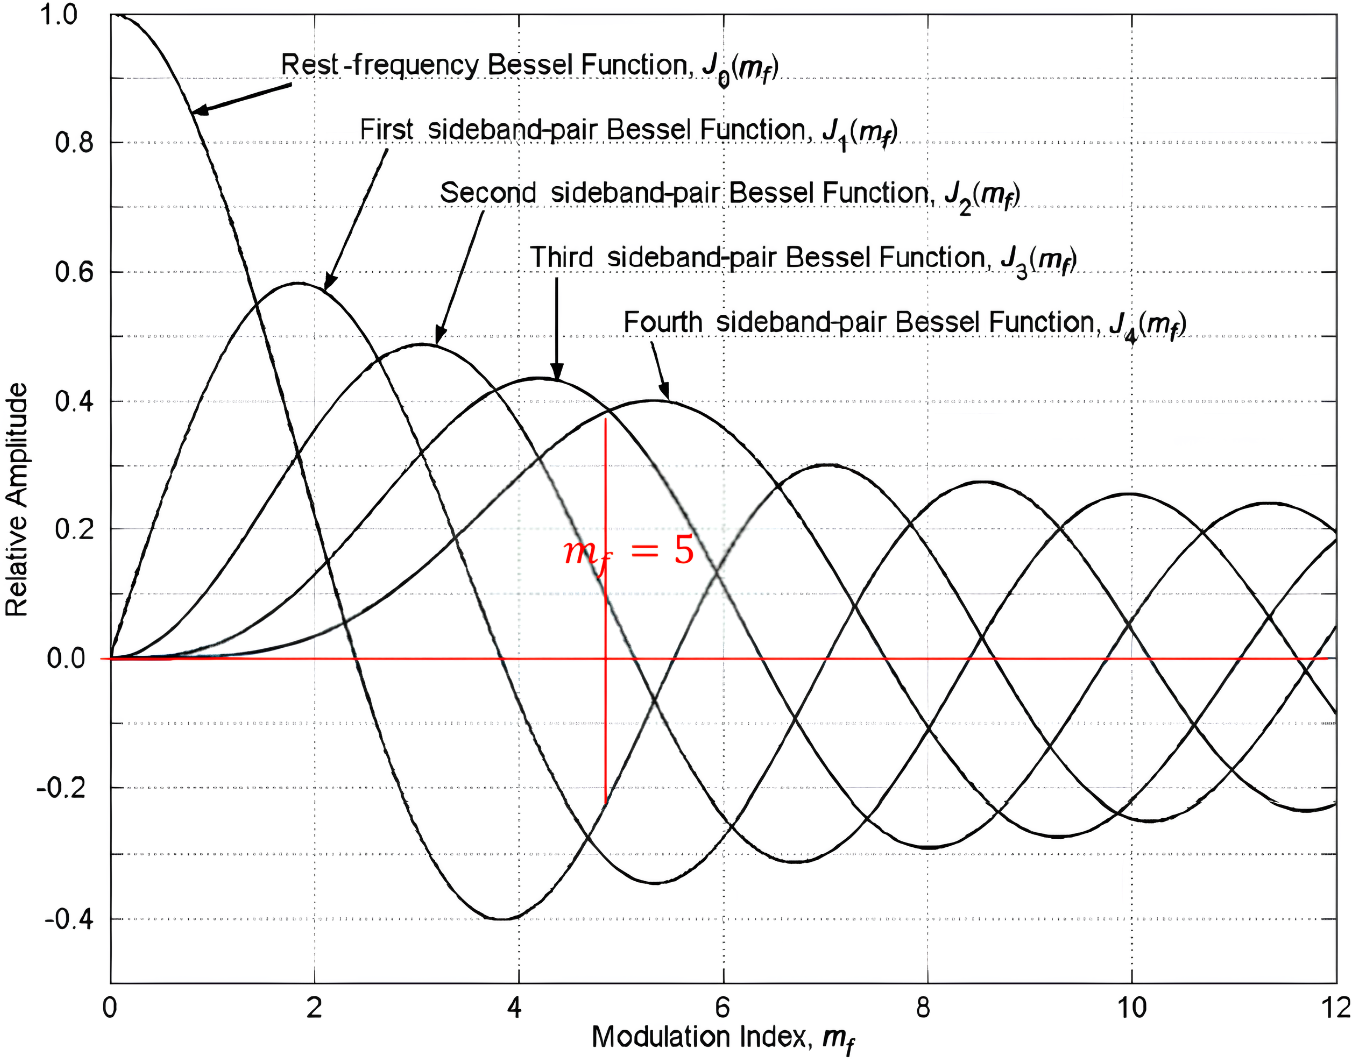
\includegraphics[width=0.625\textwidth]{imgs/bessel1.png}
\end{center}

\begin{center}
    \resizebox{0.75\textwidth}{!}{
        \tikzsetnextfilename{bessel2}
        \documentclass{standalone}

\usepackage{tikz,pgf} %and any other packages or tikzlibraries your picture needs

\begin{document}

\begin{tikzpicture}

    % Axis
    \draw[->] (0,0) -- (12,0) node[right, font=\small] {Frequency};
    \draw[->] (0,0) -- (0,7.5) node[above, font=\small] {Amplitude};


    \foreach \x [count=\xi from 0] in {1.5,3,4.5,6,7.5,9,10.5} {
            \pgfmathsetmacro{\mu}{6}  % Median of the x values
            \pgfmathsetmacro{\sigma}{2}  % Standard deviation (you can adjust this value)
            \pgfmathsetmacro{\A}{6}  % Amplitude (scaling factor)

            \pgfmathsetmacro{\y}{\A * exp(-((\x - \mu)^2) / (2 * \sigma^2))}

            % Draw the line
            \draw (\x,0) -- (\x,{\y}) node[above] {};
        }

    % Frequency labels
    \node[below, font=\small] at (1.5,0) {$f_c - 3f_m$};
    \node[below, font=\small] at (3,0) {$f_c - 2f_m$};
    \node[below, font=\small] at (4.5,0) {$f_c - f_m$};
    \node[below, font=\small] at (6,0) {$f_c$};
    \node[below, font=\small] at (7.5,0) {$f_c + f_m$};
    \node[below, font=\small] at (9,0) {$f_c + 2f_m$};
    \node[below, font=\small] at (10.5,0) {$f_c + 3f_m$};

    % fm arrow
    \draw[<->, red] (6,0.75) -- node[above, font=\small] {\textcolor{red}{$f_m$}} (7.5,0.75);

\end{tikzpicture}
\end{document}

    }
\end{center}

Ogni componente sinusoidale ha una frequenza che è un multiplo intero della frequenza di modulazione \( f_m \).
Queste componenti sono chiamate "bande laterali", e la loro ampiezza è determinata dalle funzioni di Bessel \( J_n(m_f) \).
La frequenza della portante appare come il picco centrale nello spettro (per \( n = 0 \)), con la sua ampiezza modulata da \( J_0(m_f) \).

In generale, l'ampiezza delle funzioni di Bessel (e quindi delle bande laterali) diminuisce all'aumentare di \( |n| \), anche se questo decadimento non è necessariamente monotono.
Il pattern esatto dipende dal valore dell'indice di modulazione \( m_f \), un indice di modulazione più alto distribuisce più energia nelle bande laterali di ordine superiore, allargando la banda del segnale FM,
infatti si può vedere graficamente come più è l'indice di modulazione, più è grande il numero di funzioni di Bessel di cui devo tenere conto quando rappresento lo spettro del segnale FM.
Lo spettro è simmetrico rispetto alla frequenza della portante perché \( J_{-n}(m_f) = (-1)^n J_n(m_f) \). Quindi, per ogni componente di frequenza positiva, c'è una corrispondente componente di frequenza negativa con la stessa ampiezza ma potenzialmente fase diversa (a seconda che \( n \) sia dispari o pari).
La banda di Carson approssima la larghezza di banda del segnale FM a:
\[
    B_{FM} \approx 2(\Delta f + f_{m}) = 2(m_f + 1) f_{m}
\]
\[
    \Delta f \coloneqq \text{max} \{ | f_d(t) | \} = k_f \cdot \text{max} \{ | m(t) | \}
\]
Dove \( \Delta f \) è la deviazione massima della frequenza, \( f_{m} \) è la frequenza massima del segnale modulante e \( m_f \) è l'indice di modulazione.
Questa regola stima la banda in cui è concentrata la maggior parte dell'energia del segnale FM.
Ogni segnale modulato in frequenza ha un numero infinito di bande laterali e quindi una banda infinita. Ma la maggior parte dell'energia (98\% o più) è concentrata all'interno della banda definita dalla regola di Carson. Per la radio FM mono commerciale:
\begin{align*}
    f_m      & = 15 \text{ kHz (high quality audio)}, \\
    \Delta f & = 75 \text{ kHz},                      \\
    m_f      & = 5,                                   \\
    B_{FM}   & \approx 180 \text{ kHz}.
\end{align*}

\paragraph*{Ricevitore FM}
Trascurando il rumore, il segnale ricevuto assume la forma:
\[
    \hat{v}(t) = A_c e^{j2\pi k_f \int_{-\infty}^{t} m(\tau) d\tau}
\]
Che può quindi essere demodulato differenziando la fase di \( \hat{v}(t) \):
\[
    \hat{m}(t) = \frac{1}{2\pi k_f} \frac{d}{dt} \angle \hat{v}(t)
\]


\begin{center}
    \tikzsetnextfilename{fm_receiver}
    \documentclass{standalone}

\usepackage{tikz,pgf} %and any other packages or tikzlibraries your picture needs

\begin{document}

 \begin{tikzpicture}[
            block/.style={rectangle, draw, minimum height=1cm, minimum width=1.5cm},
            node distance=1cm and 1cm,
            auto
        ]
        % Blocks
        \node[inner sep=0pt, minimum size=0pt] (source) {};
        \node[block, right=of source] (encoder) {$\angle$};
        \node[block, right=of encoder] (interp) {$\frac{d}{dt}$};

        % create a node which is above interp
        \node[above=of interp, inner sep=0pt, minimum size=0pt] (dummy1) {};
        \node[below=of interp, inner sep=0pt, minimum size=0pt] (dummy2) {};




        \node[draw, circle, right=1cm of interp] (m1) {\(\times\)};

        \draw[->] (interp) -- (m1);
        \node[below=of m1] (cos) {};
        \draw[->] (cos) -- (m1) node[midway, right] {$\frac{1}{2\pi k_f}$};


        \node[right=1cm of m1, inner sep=0pt, minimum size=0pt] (dummy3) {};


        \draw[->] (m1) -- (dummy3) node[midway, above] {$\hat{m}(t)$};



        %\draw[->] (interp) -- node[midway, above] {$x_c[n]$} (p1);

        \draw[->] (source) -- (encoder) node[midway,above] {$\tilde{v}(t)$};
        \draw[->] (encoder) -- (interp) node[midway,above] {};


    \end{tikzpicture}
\end{document}

\end{center}


Supponiamo che a causa della differenza tra trasmettitore e ricevitore ci sia adesso una frequenza $\Delta f$ (per esempio potrebbe essere anche solo 10 Hz)
\[
    v(t) = e^{j2\pi \Delta f t + j2 \pi k_f \int_{-\infty}^{t} m(\tau) d\tau}
\]

e quindi la fase sarà:
\[
    \angle v(t) = 2\pi \Delta f t + 2\pi k_f \int_{-\infty}^{t} m(\tau) d\tau
\]
da cui:
\[
    \frac{1}{2\pi k_f}  \frac{d}{dt} \angle v(t) = \frac{\Delta f}{k_f} + m(t)
\]

e da come possiamo notare, $\frac{\Delta f}{k_f}$ è solo una costante aggiunta al segnale. Come tale, sta sulla frequenza 0 che non può essere udita dall'orecchio umano. Quando la costante $\Delta f$ è grande, comunque, quando vogliamo prendere l'energia del segnale, parte del segnale potrebbe essere filtrata.% (TODO: Perché?).


\section*{Software Defined Radio (SDR)}
Le componenti di un sistema radio sono generalmente realizzate tramite dispositivi hardware analogici.
Le recenti innovazioni tecnologiche hanno permesso di implementare tali componenti direttamente in software.
All'interno di un ricevitore SDR il segnale in arrivo è convertito in formato digitale per essere processato.
La componente software permette una semplice riprogrammazione, in tal modo è possibile modificare l'elaborazione del segnale senza dover cambiare componenti fisiche del sistema.
La tecnica SDR deriva dal campo delle trasmissioni militari in cui è necessario equipaggiare i soldati con molte componenti radio per gestire le numerose comunicazioni da realizzare.
L'introduzione del SDR ha permesso di semplificare l'equipaggiamento, riducendo il numero di dispositivi necessari per supportare i protocolli radio militari.

Il campo in cui le tecniche SDR hanno portato innumerevoli vantaggi è quello della ricerca e sviluppo, perché il passaggio da design hardware a programmazione ha permesso di velocizzare i tempi di sviluppo di nuove tecnologie.

La chiave per lo sviluppo delle tecniche SDR è il miglioramento delle capacità di calcolo dei processori, perché sono in grado di applicare l'elaborazione precedentemente realizzata completamente in hardware specializzato.
Con il passaggio al software è possibile modificare l'elaborazione del segnale senza dover cambiare componenti fisiche del sistema, semplificando il processo di sviluppo e riducendo i costi, introducendo eventuali nuovi formati di modulazione, algoritmi e applicazioni.


\subsection*{Architettura RTL-SDR}
% TODO: quali sono le connessioni notevoli tra le varie componenti?
% includi immagine in pdf chiamata imgs/sdr.pdf
\begin{center}
    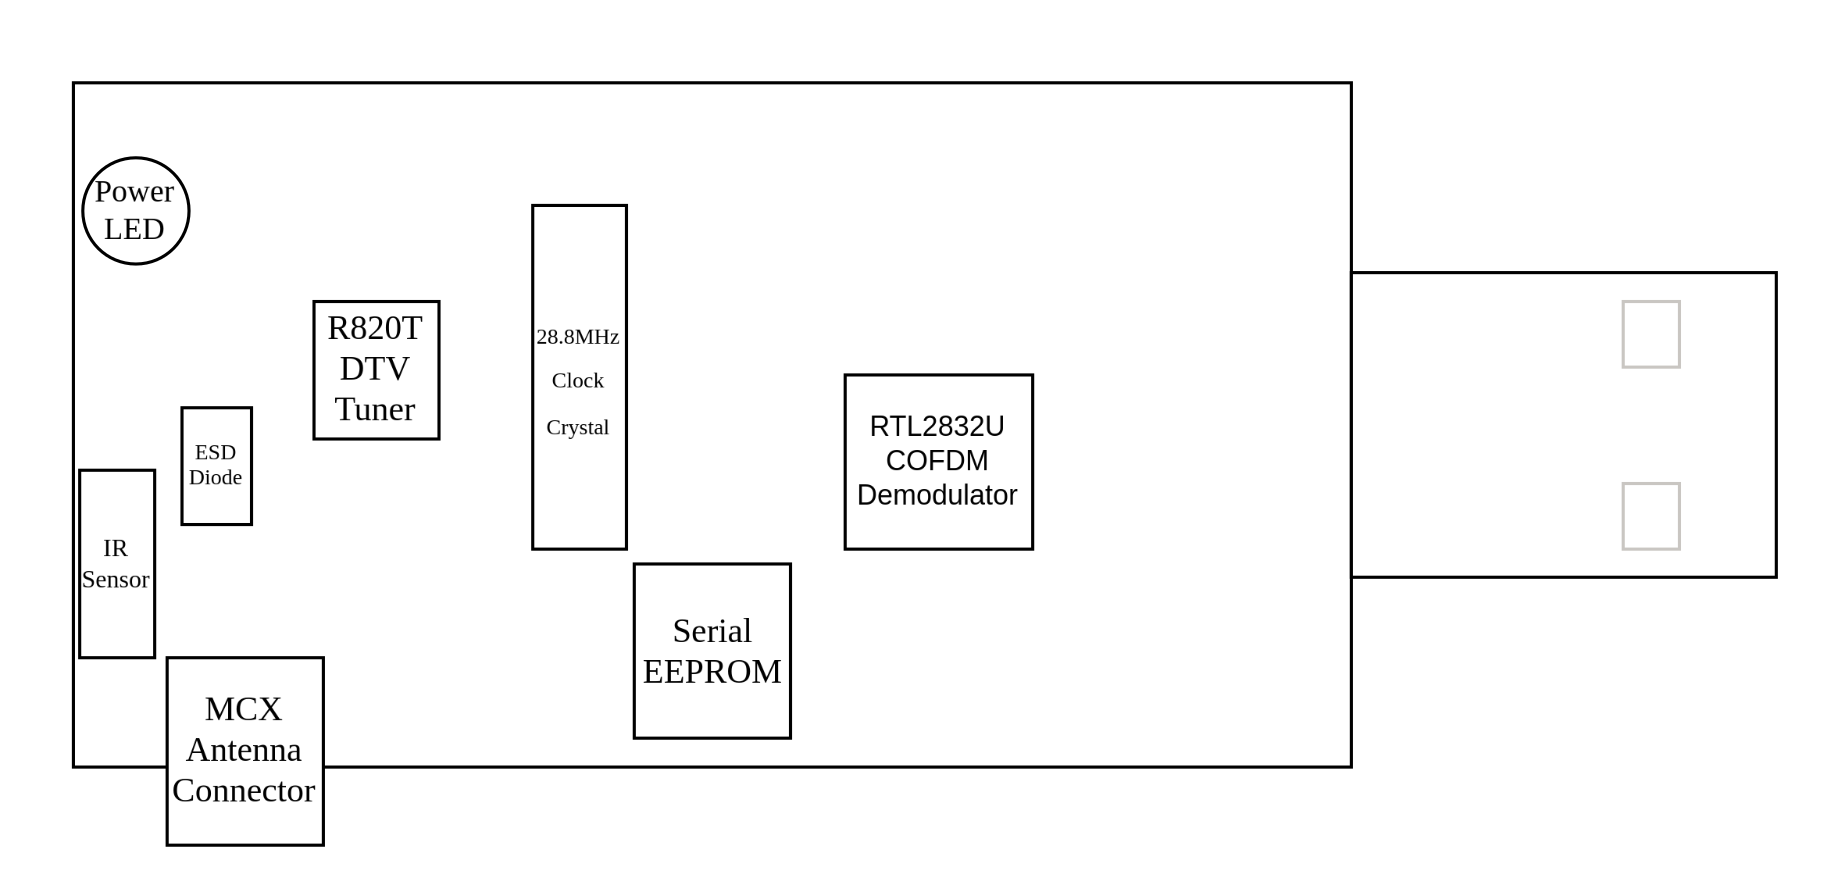
\includegraphics[width=0.8\textwidth]{imgs/sdr.png}
\end{center}


Il RTL-SDR è un dispositivo inizialmente ideato per ricevere segnale TV su un PC, che è possibile hackerare settando un bit di debug nel driver, così che invierà tutti i campioni I/Q ricevuti dall'antenna.
Il compito dell'RTL-SDR è prendere un chunk dello spettro del segnale ricevuto e convertirlo in banda base, che potrà poi essere processato dal software.
% Detailing the components of RTL-SDR

Le componenti principali sono:
\begin{itemize}
    \item \textbf{R820T DTV Tuner:} chip dedicato all'elaborazione del segnale in banda, responsabile della selezione della banda di frequenza del segnale desiderato dallo spettro RF.
    \item \textbf{28.8MHz Clock Crystal:} fornisce una frequenza di riferimento stabile per il tuner e il demodulatore, determina la banda massima che può essere ottenuta dai campioni I/Q.
    \item \textbf{RTL2832U COFDM Demodulator:} chip utilizzato per la conversione analogico-digitale, sebbene il nome "demodulator" possa essere fuorviante in questa fase non avviene nessuna demodulazione del segnale.
    \item \textbf{MCX Antenna Connector:} permette la connessione di diversi tipi di antenne.
    \item \textbf{Serial EEPROM:} memorizza i dati di configurazione del dispositivo USB.
    \item \textbf{USB 2.0 Interface:} permette la connessione con i computer per l'elaborazione successiva.
    \item Componenti aggiuntive come un \textbf{LED di alimentazione}, un \textbf{diodo ESD} e un \textbf{sensore IR} per l'interfacciamento con l'utente e la protezione del dispositivo.
\end{itemize}

Il dispositivo implementa un ricevitore super heterodyne, in cui il segnale in banda è prima trasformato in media frequenza (IF) e dopo alcune trasformazioni in banda base.
Questa doppia trasformazione è necessaria per ottimizzare l'amplificazione del segnale, più semplice a media frequenza rispetto al segnale in banda base.

\begin{center}
    \tikzsetnextfilename{rtl_chain}
    \documentclass{standalone}

\usepackage{tikz,pgf} %and any other packages or tikzlibraries your picture needs

\usepackage{pgfplots}

\usepackage[utf8]{inputenc}
\usepackage[colorlinks=true, allcolors=blue]{hyperref}
\usetikzlibrary{positioning, arrows.meta, fit, shapes}
\begin{document}


\begin{tikzpicture}[
        block/.style={rectangle, draw, minimum height=2em, minimum width=3em},
        line/.style={draw, -Latex}
    ]
        \node[block, align=center] (rfFrontEnd) {Flexible RF \\ Front End};
        \node[block, right=0.5cm of rfFrontEnd, align=center] (adConverter) {A/D Converter};
        \node[block, right=0.5cm of adConverter, align=center] (demod) {Demodulation \\ to Bband};
        \node[block, right=0.5cm of demod, align=center] (decimation) {Decimation \\ Filtering};
        \node[block, right=0.5cm of decimation, align=center] (carrierSync) {Carrier \& Timing \\ Synchronisation};
        \node[block, right=0.5cm of carrierSync, align=center] (baseband) {Baseband \\ Processing};
        \node[inner sep=0pt, outer sep=0pt, above left=0.25cm and 0.05cm of rfFrontEnd] (antenna) {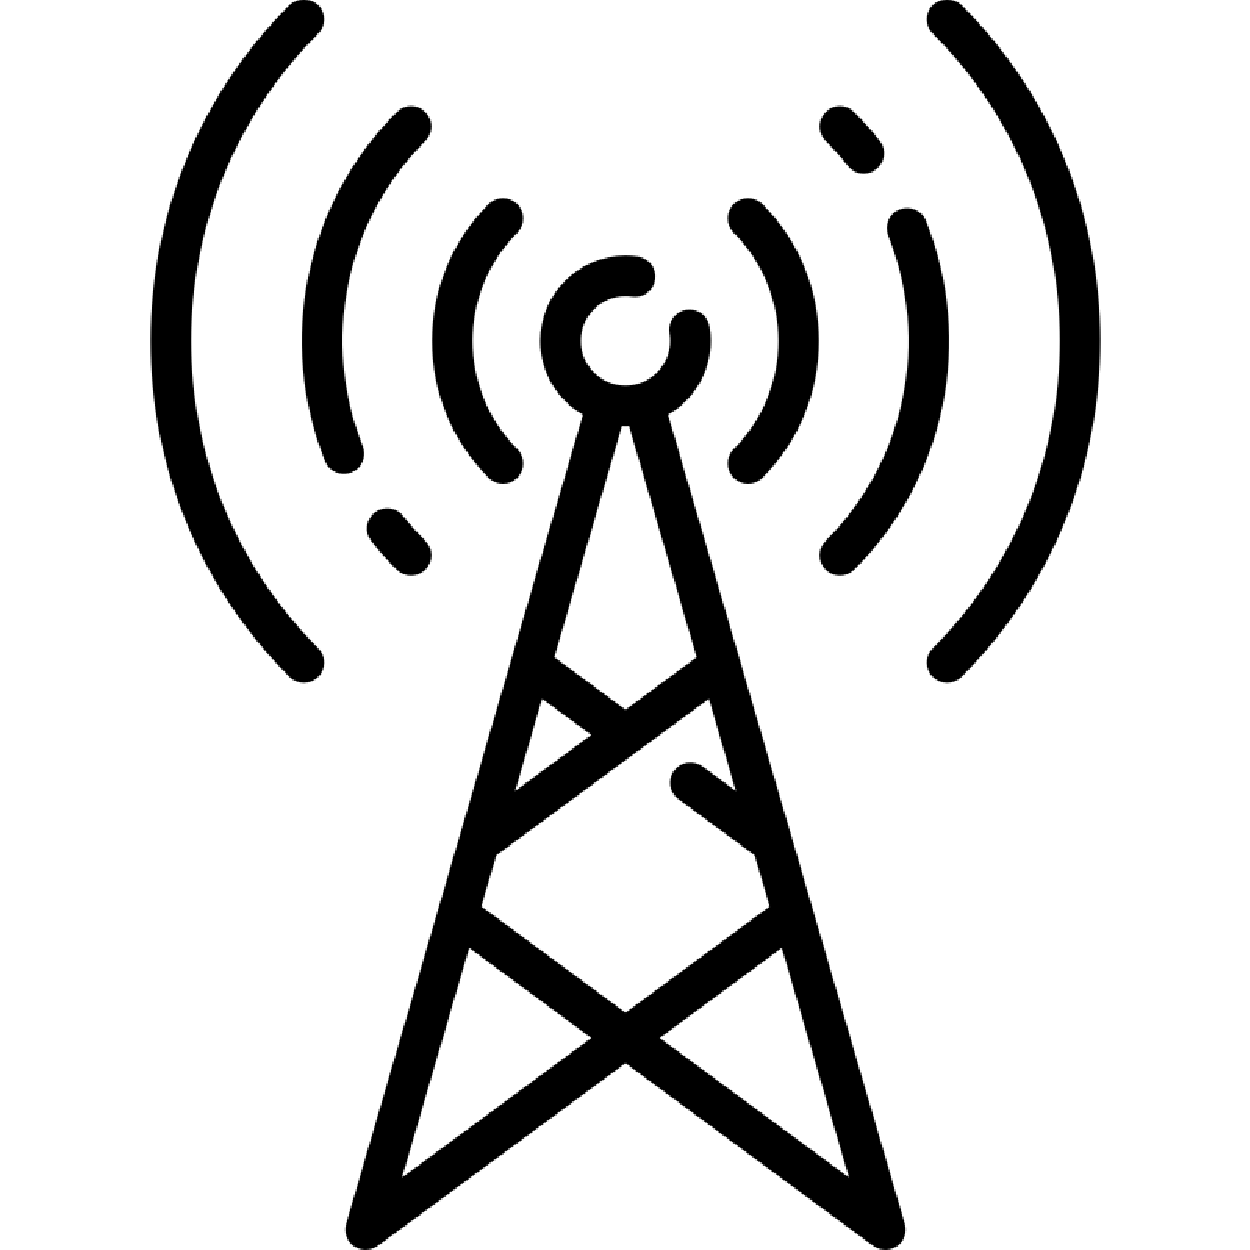
\includegraphics[width=1cm]{imgs/antenna.pdf}};

        \draw[line] (rfFrontEnd) -- (adConverter);
        \draw[line] (adConverter) -- (demod);
        \draw[line] (demod) -- (decimation);
        \draw[line] (decimation) -- (carrierSync);
        \draw[line] (carrierSync) -- (baseband);
        \draw (rfFrontEnd.west) -- ++(-0.5, 0) -- ++(0,0.5);

        \node[draw, dashed, fit=(rfFrontEnd) (adConverter) (demod) (decimation), inner sep=0.2cm, label=above:RTL-SDR Hardware] (hardware) {};
        \node[draw, dashed, fit=(carrierSync) (baseband), inner sep=0.2cm, label=above:MATLAB / Simulink design (running on computer)] (software) {};

        \node[align=left, below=0.5cm of hardware.south] (freqRange) {Range: \\ 25MHz -- 1.75GHz};
        \node[align=left, below=0.5cm of software.south] (samplingFreq) {Sampling frequency (\(f_s\)): \\ up to around 2.8MHz};

        \node[inner sep=0pt, outer sep=0pt, right=0.5cm of baseband] (output) {
\includegraphics[width=1cm]{imgs/notes.pdf}};
        \draw[line] (baseband) -- (output);
    \end{tikzpicture}

\end{document}

\end{center}
Il diagramma a blocchi per un ricevitore FM che utilizza hardware RTL-SDR tipicamente coinvolge le seguenti fasi di elaborazione:
\begin{enumerate}
\item \textbf{Antenna RF:} Cattura il segnale FM dall'aria.
\item \textbf{Flessibile Front End RF:} Filtra e amplifica il segnale RF dall'antenna.
\item \textbf{Convertitore Analogico-Digitale (ADC):} Converte il segnale RF analogico in formato digitale.
\item \textbf{Demodulazione in Banda IQ:} Il segnale digitale viene demodulato in componenti I (In-phase) e Q (Quadratura).
\item \textbf{Filtraggio di Decimazione:} Riduce la frequenza di campionamento e il rumore, mantenendo il segnale di interesse.
\item \textbf{Sincronizzazione di Portante e Temporizzazione:} Sincronizza il segnale ricevuto con il riferimento locale per una demodulazione accurata.
\item \textbf{Elaborazione della Banda Base:} Questo può coinvolgere MATLAB/Simulink in esecuzione su un computer per elaborare il segnale demodulato.
\item \textbf{Uscita della Banda Base:} Il segnale audio finale è pronto per l'ascolto.
\end{enumerate}
L'intervallo di elaborazione del segnale per questo sistema è da 25 MHz a 1,75 GHz con una frequenza di campionamento (IF) fino a circa 2,8 MHz.\begin{center}
    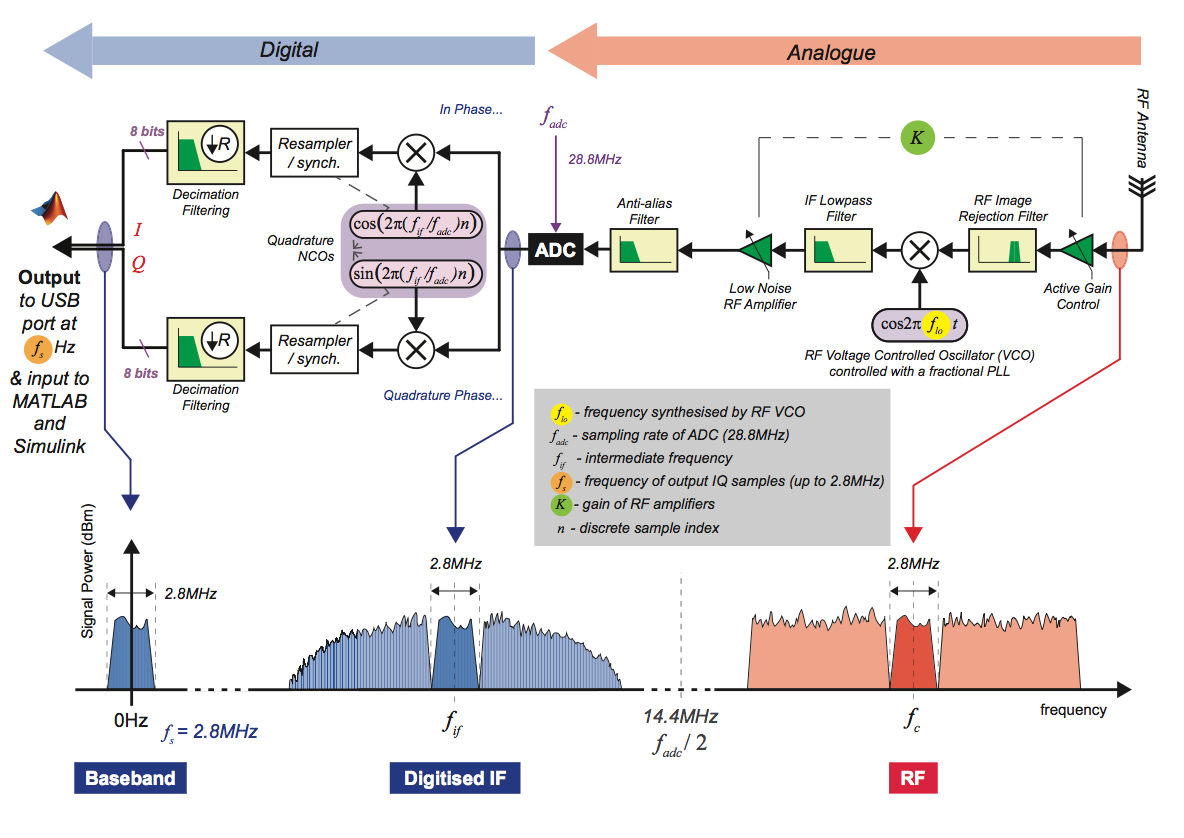
\includegraphics[width=0.75\textwidth]{imgs/rtl-sdr.png}
\end{center}


Il segnale modulato in frequenza \(s_{FM}(t)\) è espresso come:

\[
s_{FM}(t) = s_I(t) \cos (2\pi f_c t) - s_Q(t) \sin (2 \pi f_c t)
\]

La sua rappresentazione complessa è:

\[
    \tilde{s}_{FM}(t) = s_I(t) + j s_Q(t) \quad \text{con} \quad f_c = 102.5 \times 10^6 \, \si{Hz}
\]
Per portare il segnale alla banda base, nel ricevitore supereterodino si utilizza una conversione in due passaggi:
\begin{enumerate}
\item Conversione dalla frequenza della portante \(f_c\) alla frequenza intermedia \(f_{IF}\).
\item Conversione dalla frequenza intermedia \(f_{IF}\) alla banda base (BB).
\end{enumerate}
Prima di portare il segnale alla banda base, è necessario amplificarlo. Tuttavia, amplificare direttamente alla frequenza della portante richiederebbe un amplificatore con una banda molto ampia, il che è costoso. Per questo motivo, si preferisce prima convertire il segnale alla frequenza intermedia \(f_{IF}\), dove un amplificatore può essere progettato specificamente per quella frequenza.

Il processo di eterodinazione è cruciale per convertire le frequenze radio più alte in frequenze più basse, che sono più facili da amplificare e processare.
La conversione analogico-digitale avviene con un campionamento a 28.8 MS/s, rispettando il teorema di Nyquist (\(f_s > 2 (f + B)\)) per una banda di 14.4 MHz, poiché \(28.8 \si{MHz} > 2 \cdot (3.57 \si{MHz} + 2.8 \si{MHz})\).

I parametri del segnale ricevuto sono:

\[
f_c = 102.5 \times 10^6 \, \si{Hz}
\]
\[
f_{IF} = 3.57 \times 10^6 \, \si{Hz}
\]
\[
f_{LO} = f_c - f_{IF}
\]

dove \(f_{LO}\) rappresenta la frequenza dell'oscillatore locale.

\begin{center}
    \tikzsetnextfilename{sdr_receiver}
    \documentclass{standalone}

\usepackage{tikz,pgf} %and any other packages or tikzlibraries your picture needs

\usepackage{pgfplots}

\usepackage[utf8]{inputenc}
\usepackage[colorlinks=true, allcolors=blue]{hyperref}
\usetikzlibrary{positioning, arrows.meta, fit, shapes}
\begin{document}
\begin{tikzpicture}[
        block/.style={rectangle, draw, minimum height=1cm, minimum width=1.5cm},
        node distance=1cm and 1cm,
        auto
    ]

    \tikzstyle{tri} = [draw, isosceles triangle, isosceles triangle apex angle=60, shape border rotate=360, minimum height=2em]
    \node[inner sep=0pt, minimum size=0pt] (source) {};


    \node[tri, right=of source] (encoder) {};
    \node[block, right=of encoder] (interp) {BPF};
    \node[above=of interp, inner sep=0pt, minimum size=0pt] (dummy1) {};
    \node[below=of interp, inner sep=0pt, minimum size=0pt] (dummy2) {};
    \node[draw, circle, right=1cm of interp] (m1) {\(\times\)};
    \draw[->] (interp) -- (m1);
    \node[below=of m1] (cos) {};
    \draw[->] (cos) -- (m1) node[midway, right] {$\cos(2\pi(f_{c} - f_{IF})t)$};
    \node[tri, right=of m1] (dummy3) {};
    \draw[->] (m1) -- (dummy3) node[midway, above] {};
    \node[right=1cm of dummy3, inner sep=0pt, minimum size=0pt] (dummy4) {};
    \draw[->] (dummy3) -- (dummy4) node[midway, above] {};
    \draw[->] (source) -- (encoder) node[midway,above] {};
    \draw[->] (encoder) -- (interp) node[midway,above] {};

\end{tikzpicture}
\end{document}

\end{center}
\[
\begin{aligned}
s_{FM}(t) \cdot 2 \cos (2 \pi f_{LO} t) & = [s_I(t) \cos (2 \pi f_c t) - s_Q(t) \sin (2 \pi f_c t)] \cdot 2 \cos (2 \pi (f_c - f_{IF}) t) \\
& = 2 s_I(t) \cos (2 \pi f_c t) \cos (2 \pi (f_c - f_{IF}) t) - 2 s_Q(t) \sin (2 \pi f_c t) \cos (2 \pi (f_c - f_{IF}) t) \\
& = \underbrace{s_I(t) \cos(2\pi (2f_c - f_{IF}) t)}_{\text{componente ad alta frequenza}} + s_I(t) \cos(2\pi f_{IF} t) - \underbrace{s_Q(t) \sin(2\pi (2f_c - f_{IF}) t)}_{\text{componente ad alta frequenza}} - s_Q(t) \sin(2\pi f_{IF} t)
\end{aligned}
\]

Dove nell'ultimo passaggio sono state utilizzate le formule di Werner\footnote{\[
\begin{aligned}
    \cos(A)\cos(B) & = \frac{1}{2}[\cos(A+B) + \cos(A-B)] \\
    \sin(A)\cos(B) & = \frac{1}{2}[\sin(A+B) + \sin(A-B)]
\end{aligned}
\]
}. Dopo un filtro passa basso, otteniamo:
\[
= s_I(t) \cos (2 \pi f_{IF} t) - s_Q(t) \sin (2 \pi f_{IF} t)
\]





Campionando $\cos(2\pi f_{IF} t)$ si ottiene:
\[
    \cos(2\pi f_{IF} n T_s) = \cos(2\pi \frac{f_{IF}}{f_{ADC}} n)
\]

La frequenza di campionamento determina la massima banda estraibile dal segnale, ovvero 2.8 MHz.

\begin{center}
    \tikzsetnextfilename{mixer_output}
    \documentclass{standalone}

\usepackage{tikz,pgf} %and any other packages or tikzlibraries your picture needs

\usepackage{pgfplots}

\usepackage[utf8]{inputenc}
\usepackage[colorlinks=true, allcolors=blue]{hyperref}
\usetikzlibrary{positioning, arrows.meta, fit, shapes}
\begin{document}

    \begin{tikzpicture}
        \begin{axis}[
            axis lines=middle,
            width=\textwidth,
            height=8cm,
            xlabel={$f$},
            ylabel={},
            xtick={-3,-2,-1,0,1,2,3},
            xticklabels={$-f_{IF}-W$, $-f_{IF}$, $-f_{IF}+W$, $0$, $f_{IF}-W$, $f_{IF}$, $f_{IF}+W$},
            ytick=\empty,
            xmin=-4,
            xmax=4,
            ymin=0,
            ymax=1,
            clip=false
        ]

        \pgfmathsetmacro{\fIF}{2}
        \pgfmathsetmacro{\W}{1}

        \addplot[domain=-\fIF-\W:-\fIF+\W, samples=100, black, thick] 
            ({x}, {((sqrt(-15129*(x+\fIF)^2 + 1968*(x+\fIF)*sin(deg(15*(x+\fIF)))^3 - 64*sin(deg(15*(x+\fIF)))^6 + 14400))/(120))} - 0.269 );
        \addplot[domain=\fIF-\W:\fIF+\W, samples=100, black, thick] 
            ({x}, {((sqrt(-15129*(x-\fIF)^2 + 1968*(x-\fIF)*sin(deg(15*(x-\fIF)))^3 - 64*sin(deg(15*(x-\fIF)))^6 + 14400))/(120))} - 0.269 );

        \draw[->,thick] (axis cs:-4,0) -- (axis cs:4,0) node[right] {};
        \draw[->,thick] (axis cs:0,0) -- (axis cs:0,1);

        \end{axis}
    \end{tikzpicture}

\end{document}

\end{center}
% TODO: cos'è il mixer?
Nella figura è rappresentato il segnale in uscita dal mixer, con frequenza intermedia $f_{IF} = 3.57$ MHz e banda $W = 1.4$ MHz.

Ogni sample è composto da 8 bit. I sample del segnale campionato seguono un percorso parallelo per estrarre la commponente in fase e in quadratura. Entrambi i rami effettuano la conversione da media a frequenza a banda base.
Avvengono una serie di operazioni che permettono di estrarre la banda che sarà rappresentata dai sample I/Q in uscita da ques'ultima fase tramite interfaccia USB.
La fase di decimation permette di adattare il campionamente  del segnale al valore richiesto dell'utente. Il rate massimo è circa 2.8 MS/s.
Lo spettro di frequenza in grado di essere captato dal dispositivo risulta approssimativamente (TODO).
Bisogna comunque tenere in considerazione che la banda limitata a 2.8 MHz non permette di estrarre informazioni di modulazioni che richiedano una banda superiore, ad esempio il Wi-Fi.


\paragraph*{Ricezione radio FM}
\begin{center}
    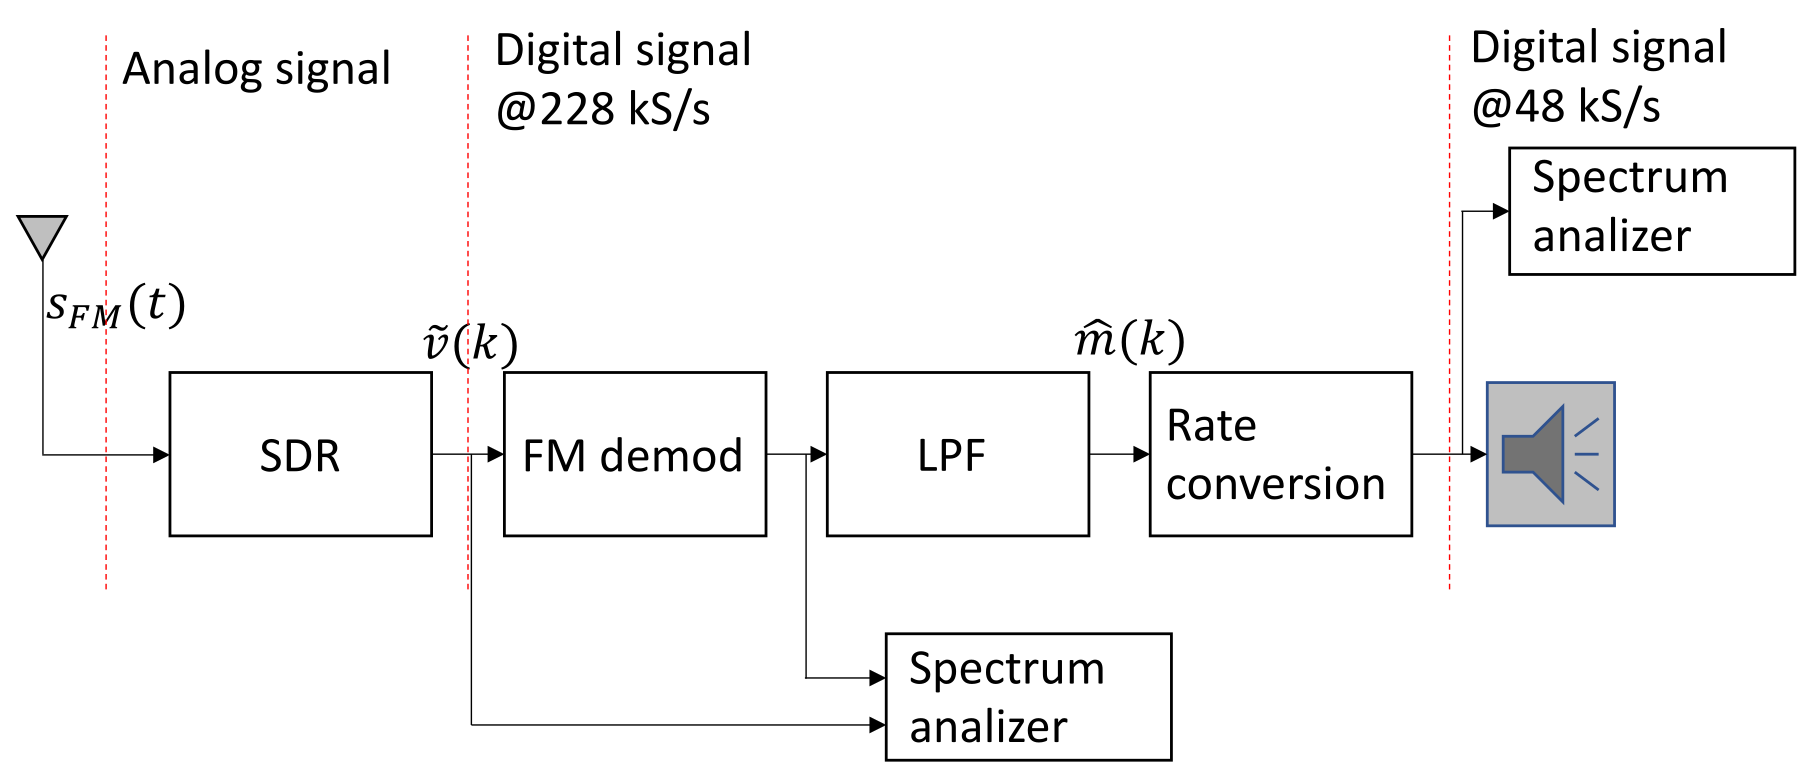
\includegraphics[width=0.75\textwidth]{imgs/fm_receiver_impl.jpg}
\end{center}
I simboli I/Q digitali ricevuti dal SDR richiedono una demodulazione per essere convertiti nell'informazione trasmessa. In particolare per la radio FM si considera
\[
    m(t) = L(t) + R(t)
\]
segnale FM mono, normalizzato ad 1, ovvero $\max{m(t)} = 1$ e quindi $\Delta f = k_f$.


L'inviluppo complesso del segnale ricevuto assume la forma:

\[
    \tilde{v}(t) = A_c e^{j2\pi k_f \int_{-\infty}^{t} m(\tau) d\tau}
\]

Campionando in $T_s$ si ottiene:
\[
    \tilde{v}(kT_s) = \tilde{v}[k] = A_c e^{j2\pi k_f \int_{-\infty}^{kT_s} m(\tau) d\tau}
\]

che può essere approssimato a 
\[
    \tilde{v}[k] \approx A_c e^{j2\pi k_f \sum_{\ell = -\infty}^{k} m[\ell] \ T_s}
\]

moltiplicando per il coniugato del campione precedente si ottiene
\[
    \tilde{v}[k] \ \tilde{v}^*[k-1] \approx A_c^2 e^{j2\pi k_f \sum_{\ell = -\infty}^{k} m[\ell] \ T_s} e^{-j2\pi k_f \sum_{\ell = -\infty}^{k-1} m[\ell] \ T_s} = A_c^2 e^{j2\pi k_f m[k] \ T_s}
\]

da cui:
\[
    \tilde{m}[k] = \frac{1}{2\pi k_f T_s} \angle \left( \tilde{v}[k] \ \tilde{v}^*[k-1] \right)
\]



\subsection*{Implementazione in MATLAB}
In questa sezione ci limitiamo a riportare l'implemenetazione in MATLAB di ciò finora discusso. Per prima cosa inizializziamo i parametri:
\begin{minted}{matlab}
%% PARAMETERS
rtlsdr_id        = '0';                     % stick ID
rtlsdr_fc        = 102.5e6;                 % tuner centre frequency in Hz
rtlsdr_fs        = 228e3;                   % tuner sampling rate (fixed to 228 kHz)
rtlsdr_frmlen    = 1000 * 38;               % output data frame size (must be a multiple of 5)
rtlsdr_gain      = 50;                      % tuner gain in dB
rtlsdr_datatype  = 'double';                % output data type
audio_fs         = 48e3;                    % audio output sampling rate
simTime          = 30;                      % simulation time in seconds
freqDev          = 75e3;
numSampleSim     = simTime * rtlsdr_fs;

sdrOn = 1;

% load filter coefficients from a file
load filters.mat

% low pass filter @ 15 kHz
obj_lpf = dsp.FIRFilter('Numerator', numerator);

% link to a physical rtl-sdr
if sdrOn == 1
    obj_rtlsdr = comm.SDRRTLReceiver(...
        'RadioAddress', rtlsdr_id, ...
        'CenterFrequency', rtlsdr_fc, ...
        'EnableTunerAGC', false, ...
        'TunerGain', rtlsdr_gain, ...
        'SampleRate', rtlsdr_fs, ...
        'SamplesPerFrame', rtlsdr_frmlen, ...
        'OutputDataType', rtlsdr_datatype);
else
    load dumpFM
    % adapt the length of dump to rtlsdr_frmlen
    lengthDump = length(dump);
    lengthDump = lengthDump - rem(length(dump), rtlsdr_frmlen);
    numSampleSim = min(numSampleSim, lengthDump);
end

% resamples the signal rate from rtlsdr_fs kS/s to audio_fs kS/s
sampRateAd = dsp.SampleRateConverter('Bandwidth', 15e3, ...
    'InputSampleRate', rtlsdr_fs, 'OutputSampleRate', audio_fs, ...
    'StopbandAttenuation', 50);

% spectrum analyzer @ rtlsdr_fs
obj_spectrumUp = dsp.SpectrumAnalyzer(...
    'Name', 'Spectrum Analyzer @RTL frequency', ...
    'Title', 'RTL frequency signal spectrum', ...
    'SpectrumType', 'Power density', ...
    'FrequencySpan', 'Full', ...
    'ShowLegend', true, ...
    'SampleRate', rtlsdr_fs, ...
    'SpectralAverages', 100);

% spectrum analyzer @audio_fs
obj_spectrumAudio = dsp.SpectrumAnalyzer(...
    'Name', 'FM Audio signal spectrum', ...
    'Title', 'Audio Signal Spectrum', ...
    'SpectrumType', 'Power density', ...
    'FrequencySpan', 'Full', ...
    'ShowLegend', true, ...
    'SampleRate', audio_fs, ...
    'SpectralAverages', 100);

% audio player
player = audioDeviceWriter('SampleRate', audio_fs);
\end{minted}

Infine eseguiamo la demodulazione su \texttt{rtlsdr\_frmlen} campioni, utilizzando la formula precedentemente ricavata. Assumendo \( m(t) \) normalizzato a un valore massimo pari a 1, otteniamo:
\[
    \tilde{m}[k] = \frac{f_s}{2\pi \Delta f} \angle \left( \tilde{v}[k] \ \tilde{v}^*[k-1] \right)
\]
Per eseguirla, utilizzando un vettore ausialiare che conterrà gli stessi valori dei campioni, ma shiftati di una posizione e coniugati, ottenendo il seguente codice:
\begin{minted}{matlab}
numSamp = 0;
lastSample = 0;

% the RTL keeps passing signal samples until the exit condition is met
while numSamp < numSampleSim
    % sdr signal samples
    if sdrOn == 1
        % every time step is called, MATLAB polls the RTL-SDR stick and downloads the 
        % content of the shift register
        sigRx = step(obj_rtlsdr);
    else
        sigRx = dump(numSamp + 1:numSamp + rtlsdr_frmlen);
    end

    % one-sample delayed version of the received signal
    sigRxDel = [lastSample; sigRx(1:end - 1, 1)];

    % modulating signal m(t)
    rxData = rtlsdr_fs / (2 * pi * freqDev) * angle(sigRx .* conj(sigRxDel));

    % signal spectrum before and after the differentiator
    step(obj_spectrumUp, [sigRx, rxData])

    % Low-pass filtering of the BB signal
    LPRBBUp = step(obj_lpf, rxData);

    % rate conversion @ audio_fs
    LPRBB = sampRateAd(LPRBBUp);

    % Audio signal spectrum sampled @ audio_fs
    step(obj_spectrumAudio, LPRBB)

    % play audio stereo signal
    player(LPRBB);

    % update of the rtlsdr number of samples
    numSamp = numSamp + rtlsdr_frmlen;
    % track the last element of the incoming signal vector to create the
    % one-sample delayed version of the signal
    lastSample = sigRx(end);
end
\end{minted}
\section*{Transmitting a Sequence of Bits}

% Introduction to transmitting bits as an analog signal
When it comes to transmitting a sequence of bits as an analog signal, a direct approach might involve representing each bit by a delta function. However, such a train of delta functions occupies infinite bandwidth. To make this practical for transmission:

\begin{itemize}
    \item The bit sequence \( \{d_k\} \) is first passed through a low-pass filter to limit the bandwidth.
    \item The filtered signal can then be modulated onto a carrier frequency for transmission through the air.
\end{itemize}

\section*{Modeling Bit Transmission}

% Modelling each bit for transmission
Each bit in the sequence can be modeled as an equiprobable random variable, where:
\[
P(d_k = 0) = P(d_k = 1) = \frac{1}{2}
\]
and the expected value is \( E\{d_k\} = \frac{1}{2} \).

% Energy saving by transmitting 0-mean information symbols
To conserve energy, it is more efficient to transmit information symbols that have zero mean. Thus, bits are mapped to information symbols as follows:
\[
a_i =
\begin{cases}
  0 \rightarrow -1,\\
  1 \rightarrow 1.
\end{cases}
\]
This mapping results in a simple bipolar non-return-to-zero (NRZ) line code where each bit is represented by a positive or negative level.

% Mapping information symbols to transmit more than one bit
By extending this principle, one information symbol can be used to represent more than a single bit, a technique that leads to more advanced modulation schemes such as QPSK, 16-QAM, etc., which map multiple bits to a single symbol.

\subsection*{Equation for Bit Sequence Transmission}
Representing a bit sequence for transmission involves the summation of scaled and shifted delta functions:
\[
\sum_{\ell} d_{\ell}\delta(t - \ell T_b)
\]
where \( \delta(t) \) is the delta function, and \( T_b \) is the bit period.


\section*{Pulse Amplitude Modulation}

% Introduction to PAM
Pulse Amplitude Modulation (PAM) is achieved by:
\begin{enumerate}
    \item Mapping the bits \( \{d_k\} \) to information symbols \( \{a_i\} \).
    \item Filtering the symbols with a low-pass filter with impulse response \( g_r(t) \).
\end{enumerate}
The resulting PAM signal is expressed as:
\[ s_{PAM}(t) = \sum_i a_i g_r(t - iT) \]
where \( T \) is the symbol duration.

% Bit and symbol duration in PAM
It is possible for a mapper to map a sequence of \( m \) bits onto a single information symbol, resulting in different bit duration \( T_b \) and symbol duration \( T \).

\subsection*{Pulse Amplitude Modulation Signal}

% Detailed explanation of the PAM signal
The signal \( s_{PAM}(t) \) is a real baseband signal that can be modulated at any carrier frequency \( f_c \). The modulation process can be described as:
\[ s_{PAM}(t) = \sum_i a_i g_r(t - iT) \cos(2\pi f_c t) \]

% Equivalence to an analog DSB signal
The PAM signal is equivalent to an analog double sideband (DSB) signal where \( m(t) \) is the modulating (and complex envelope) signal:
\[ m(t) = \sum_i a_i g_r(t - iT) = s_{PAM}(t) \]

% Baseband equivalent of the PAM signal
For simplification, the baseband equivalent signal is considered:
\[ s_{PAM}(t) = \sum_i a_i g_r(t - iT) \]
Here, \( s_{PAM}(t) \) refers to the complex envelope of the PAM signal, and \( g_r(t) \) is the impulse response of the low-pass filter used in the modulation process.

\section*{PAM: Symbol Mapping}

% Description of the mapper in symbol mapping
The mapper in a PAM system associates a sequence of \( m \) bits \( \{d_k\} \) to a single symbol \( a_i \). For each information symbol representing \( m \) bits, the symbol constellation contains \( M = 2^m \) symbols, which is always a power of two.

% Zero mean for mapped symbols
Typically, the mapping is designed so that the expected value of the information symbols is zero:
\[ E\{a_i\} = 0 \]

% Efficiency and energy considerations
The efficiency of spectrum usage increases with the constellation size \( M \), allowing more bits per symbol. However, this also increases the average energy required to transmit a bit.

\subsection*{Bit and Symbol Rates}

% Bit generation rate
The source generates bits at a rate \( R_b = \frac{1}{T_b} \), where \( T_b \) is the bit time.

% Relationship between symbol time and bit time
Given the bit time \( T_b \), and that each symbol maps \( m \) bits, the symbol time \( T \) is given by:
\[ T = mT_b = \log_2 M \cdot T_b \]

% Symbol rate in terms of bit rate
Consequently, the symbol rate \( R \) is \( m \) times smaller than the bit rate \( R_b \):
\[ R = \frac{1}{T} = \frac{1}{mT_b} = \frac{R_b}{m} = \frac{R_b}{\log_2 M} \]

\subsection*{Symbol Constellations}

% Visualization of different symbol constellations
Constellation diagrams for different values of \( m \) illustrate how bits are mapped to symbols:
\begin{itemize}
    \item For \( M = 2 \) (or \( m = 1 \)), the constellation points are typically at -1 and +1.
    \item For \( M = 4 \) (or \( m = 2 \)), the points are located at -3, -1, +1, and +3.
    \item As \( M \) increases to 8 (or \( m = 3 \)), the constellation points represent 3-bit combinations, and so on.
\end{itemize}
This demonstrates how the modulation scheme can be scaled to map longer sequences of bits onto more complex symbols, improving data rate at the cost of requiring a higher signal-to-noise ratio for reliable transmission.


\section*{Stochastic Processes}

% Definitions of deterministic and stochastic processes
A \textbf{deterministic process} is characterized by a specific mathematical relation. In contrast, a \textbf{stochastic process} results from numerous independent causes and is described in terms of probabilities and statistical averages.

% Description of a stochastic process as a set of random variables
A stochastic process is a collection of random variables indexed in time, representing the evolution of some system over time:
\begin{itemize}
    \item Let \( \xi \) represent the random outcome of an experiment. For each outcome, we assign a time-dependent waveform \( X(t, \xi) \).
    \item The collection of these waveforms, as \( \xi \) varies over all possible outcomes of the experiment, forms a stochastic process.
    \item At any fixed time \( t = t_0 \), \( X(t_0, \xi) \) is a specific realization of the random variable.
    \item Over time, the ensemble of these realizations constitutes the stochastic process \( X(t) \).
\end{itemize}

% Mathematical representation of stochastic processes
Stochastic processes are used to model systems where uncertainty or randomness is inherent, such as noise in communication systems, stock market prices, or any system affected by random inputs.

\subsection*{Example of Stochastic Processes}
An example of a stochastic process in signal processing could be the thermal noise in a resistor, which is a random signal that can be characterized by its statistical properties, like mean and variance, over time.

\section*{Distribution and Probability Density Function}

% Distribution function for a stochastic process
For a stochastic process \( X(t) \), at any fixed time \( t_0 \), the value \( X(t_0) \) is a random variable. The distribution function for \( X(t_0) \) is given by:
\[ F_{X(t_0)}(x) = \Pr\{X(t_0) \leq x\} \]
which depends on the specific time instant \( t_0 \). Different instances in time yield different distribution functions, hence different random variables.

% Probability density function
The first-order probability density function (pdf) is the derivative of the distribution function:
\[ f_{X(t_0)}(x) = \frac{d}{dx}F_{X(t_0)}(x) \]
This pdf describes the likelihood of the random variable \( X(t_0) \) taking on a value at or near \( x \).

\section*{Independence}

% Independence in stochastic processes
An \textbf{independent} stochastic process means that the random variables \( X(t_1), \ldots, X(t_n) \) at any \( n \) different times are statistically independent. For such processes, the joint distribution function can be expressed as the product of the individual distributions:
\[ F_{X(t_1),\ldots,X(t_n)}(x_1, \ldots, x_n) = F_{X(t_1)}(x_1) \cdots F_{X(t_n)}(x_n) \]

% Probability density function for independent stochastic processes
And the joint probability density function is similarly the product of the individual densities:
\[ f_{X(t_1),\ldots,X(t_n)}(x_1, \ldots, x_n) = f_{X(t_1)}(x_1) \cdots f_{X(t_n)}(x_n) \]

\subsection*{Implications of Independence}

% Explanation of the significance of independence
Independence implies that the occurrence of a particular value at time \( t_1 \) does not influence the likelihood of any value occurring at another time \( t_2 \). This property is crucial for analyzing and designing communication systems, signal processing algorithms, and in various fields like finance and natural sciences.


\section*{Mean and Autocorrelation}

% Definition of the mean of a stochastic process
The mean of a stochastic process \( X(t) \) at time \( t_0 \) is defined by the expected value:
\[ \mu_X(t_0) = E\{X(t_0)\} = \int_{-\infty}^{+\infty} x f_{X(t_0)}(x) \, dx \]
This mean value is generally a function of the time index \( t \).

% Autocorrelation function
The autocorrelation function \( R_{XX}(t_1, t_2) \) of a process:
\[ R_{XX}(t_1, t_2) = E\{X(t_1)X^*(t_2)\} = \int_{-\infty}^{+\infty} \int_{-\infty}^{+\infty} x_1 x_2 f_{X(t_1),X(t_2)}(x_1, x_2) \, dx_1 dx_2 \]
represents the correlation between the values of the process at two different times \( t_1 \) and \( t_2 \).

\section*{Stationarity}

% Stationary processes definition
A stationary process has statistical properties that do not change over time, meaning they are invariant to shifts in the time index.

% First-order stationarity
First-order stationarity implies that the statistical properties of \( X(t_0) \) and \( X(t_0 + c) \) are the same for any shift \( c \):
\[ f_{X(t_0)}(x) = f_{X}(x) \]
implying that the mean is constant and independent of \( t_0 \).

% Second-order stationarity
Second-order stationarity extends this concept to the second moment, indicating that the joint distribution of \( (X(t_1), X(t_2)) \) and \( (X(t_1 + c), X(t_2 + c)) \) is the same, leading to an autocorrelation function that depends only on the time difference:
\[ f_{X(t_1),X(t_2)}(x_1, x_2) = f_{X}(x_1, x_2, t_2 - t_1) \]
Thus, \( R_{XX}(t_1, t_2) \) becomes \( R_{XX}(\tau) \) with \( \tau = t_2 - t_1 \).

\subsection*{Autocorrelation Function Example}
Given a stationary process, the autocorrelation function evaluated at \( \tau = 0 \) represents the average power of the signal, often denoted as \( R_{XX}(0) \).


\section*{Wide Sense Stationarity}

% Definition of wide-sense stationarity (WSS)
Wide-sense stationarity (WSS) is a less stringent form of stationarity that a process \( X(t) \) can exhibit. A process is considered WSS if:
\begin{enumerate}
    \item The mean \( E\{X(t)\} \) is constant over time, denoted \( \mu_X \).
    \item The autocorrelation function \( E\{X(t_1),X(t_2)\} \) depends only on the time difference \( \tau = t_2 - t_1 \) and is denoted \( R_{XX}(\tau) \).
\end{enumerate}
These conditions ensure that the first two moments (mean and autocorrelation) do not vary with time.

% Implications of WSS
For a wide-sense stationary process:
\begin{itemize}
    \item The mean of the process is a constant, which simplifies analysis and processing.
    \item The autocorrelation function only depends on the time difference \( \tau \), not on the specific times \( t_1 \) or \( t_2 \), implying that the statistical structure of the process does not change over time.
\end{itemize}

\section*{Autocorrelation Function}

% Understanding the autocorrelation function
The autocorrelation function \( R_{XX}(t_1, t_2) \) quantifies the interrelationship between values of the process at different times, reflecting how the process values at one time are statistically related to values at another time:
\[ R_{XX}(t_1, t_2) = E\{X(t_1)X^*(t_2)\} \]

% Rate of change in the stochastic process and its effect on autocorrelation
The behavior of \( X(t) \) affects the autocorrelation:
\begin{itemize}
    \item A stochastic process that changes slowly over time will have an autocorrelation function that decreases slowly from its maximum at \( R_{XX}(0) \).
    \item Conversely, if the process fluctuates rapidly, the autocorrelation function will drop off more quickly.
\end{itemize}

% Graphical representation
% (Assuming a figure is provided)
% \begin{figure}[ht]
% \centering
% \includegraphics[width=0.8\textwidth]{path_to_autocorrelation_figure}
% \caption{Example of autocorrelation functions for slowly and rapidly fluctuating stochastic processes.}
% \label{fig:autocorrelation}
% \end{figure}
\section*{Power Spectral Density}

% Definition of Power Spectral Density
The power spectral density (PSD) \( S_{XX}(f) \) of a wide-sense stationary (WSS) stochastic process \( X(t) \) quantifies the distribution of power across frequency components. It is typically measured in watts per hertz (W/Hz).

% Wiener-Khinchine Theorem
According to the Wiener-Khinchine theorem, the PSD is obtained by taking the Fourier transform of the autocorrelation function \( R_{XX}(\tau) \):
\[ S_{XX}(f) = \mathcal{F}\{R_{XX}(\tau)\} = \int_{-\infty}^{+\infty} R_{XX}(\tau)e^{-j2\pi f\tau} \, d\tau \]

% Signal power calculation using PSD
The total power \( P_X \) of the signal \( X(t) \) can be computed by integrating the PSD over all frequencies:
\[ P_X = \int_{-\infty}^{+\infty} S_{XX}(f) \, df \]

This integration of the PSD over frequency provides a measure of the total energy present in the signal across the entire frequency spectrum.


\section*{PAM: Power Spectral Density}

% Modeling of a PAM signal as a stochastic process
A PAM signal is modeled as a stochastic process because the symbols \( \{a_i\} \) are samples of a discrete-time discrete-state stochastic process. This process is typically assumed to be stationary and independent.

% Bandwidth and PSD of a stochastic process
The bandwidth occupied by a stochastic process is measured by its power spectral density, which is the Fourier transform of its autocorrelation function.

% PSD of the complex envelope of a PAM signal
The PSD of the complex envelope \( s(t) \) of a PAM signal is given by:
\[ S_s(f) = \frac{1}{T} S_a(f) |G_T(f)|^2 \]
where \( S_a(f) \) is the PSD of \( a_i \), and \( G_T(f) \) is the frequency response of the transmit filter \( g_T(t) \).

% Explanation of PAM signal PSD
The PSD \( S_s(f) \) provides a spectral representation of how the power of a PAM signal is distributed across different frequency components. The transmit filter's frequency response shapes the spectrum of the transmitted signal.


\section*{PAM: Power Spectral Density (continued)}

% Computing the PSD of ai
The PSD \( S_a(f) \) for the information symbols \( a_i \) in a PAM system is computed from the Fourier transform of the autocorrelation function \( R_a(m) \) of the symbols, assuming they form a stationary, discrete, independent process:
\[ R_a(m) = E\{a_i a_{i+m}\} = 
\begin{cases} 
A & \text{for } m = 0, \\
0 & \text{for } m \neq 0,
\end{cases} \]
where \( A = E\{a_i^2\} \) is the average power of the symbols.

% PSD of the PAM signal with zero-mean symbols
When the symbols are zero-mean (\( E\{a_i\} = 0 \)), the autocorrelation function becomes a delta function, and its Fourier transform is a constant, \( S_a(f) = A \). Thus, the PSD of the PAM signal is given by:
\[ S_s(f) = \frac{A}{T} |G_T(f)|^2 \]
where \( G_T(f) \) is the frequency response of the transmit filter \( g_T(t) \).

% Explanation of the PSD of a PAM signal
This PSD represents the power distribution across frequencies for the PAM signal, taking into account the shaping effect of the transmit filter on the signal's spectrum.


\section*{PAM: Pulse Shaping}

% Influence of the transmit filter on the PAM signal
The low-pass transmit filter is crucial in determining the bandwidth and spectrum of the PAM signal. The filter's impulse response, \( g_T(t) \), directly influences the shape of the transmitted pulses.

% Impact of pulse duration on spectrum and energy distribution
If the pulse shape \( g_T(t) \) is longer than the symbol time \( T \), this leads to a more compact spectrum, but the energy of one symbol may spread over multiple symbol intervals, potentially causing interference.

% Optimal pulse shaping for bandwidth efficiency
The most compact spectrum for a PAM signal is obtained when the transmit filter's frequency response \( G_T(f) \) is a rectangular function, which in the time domain corresponds to:
\[ g_T(t) = \frac{1}{T} \text{sinc}\left( \frac{t}{T} \right) \]
This sinc function, spanning several symbol intervals, ensures that each symbol minimally interferes with adjacent symbols.

% Intersymbol interference (ISI)
The phenomenon where one symbol affects the subsequent symbols is known as intersymbol interference (ISI). Proper pulse shaping, such as using the sinc function, can help mitigate ISI and allow for more efficient use of the communication channel.


\section*{PAM: Occupied Bandwidth}

% Trade-off in pulse shaping
When designing a PAM system, a trade-off is necessary between having a compact spectrum and avoiding interference:
\begin{itemize}
    \item A compact spectrum leads to a large amount of interference in the time domain, exemplified by choosing a rectangular (\texttt{rect}) shape in the frequency domain, corresponding to a sinc function in the time domain.
    \item A wide spectrum ensures that most of the symbol energy is within one symbol interval, which can be achieved by selecting a \texttt{rect} function in the time domain and consequently a sinc function in frequency domain.
\end{itemize}

\section*{PAM: Receiver Architecture}

% PAM system block diagram
The PAM system block diagram consists of:
\begin{enumerate}
    \item A source generating a sequence of bits \( \{d_k\} \).
    \item A PAM transmitter (Tx) encoding the bits into a signal \( s(t) \).
    \item A channel through which the signal propagates, typically modeled as a linear time-invariant (LTI) system with impulse response \( h(t) \).
    \item Additive white Gaussian noise (AWGN) introduced by the channel, denoted \( w(t) \), with a zero-mean and a power spectral density \( S_w(f) \).
    \item A PAM receiver (Rx) that receives the signal \( r(t) \) and aims to reconstruct the original bit sequence.
\end{enumerate}

% Channel and noise characteristics
In an ideal scenario, the channel's impulse response is a delta function \( \delta(t) \), indicating no distortion. The noise term \( w(t) \) is assumed to be white, which implies a constant PSD across all frequencies, and Gaussian, implying that its amplitude follows a normal distribution.

% Receiver's task
The key task for the receiver is to recover the transmitted bit sequence from the received signal \( r(t) \), which includes dealing with the effects of the channel and the noise.


\section*{PAM: Receiver Architecture}

% Steps of the PAM Receiver operation
The PAM receiver's operation consists of the following steps:
\begin{enumerate}
    \item Filtering noise and interference from the received signal \( r(t) \) with a low-pass filter \( G_R(f) \).
    \item Sampling the filtered signal \( x(t) \) once per symbol time \( T \) to obtain samples \( x(m) \).
    \item Recovering the transmitted bits from the signal samples \( x(m) \).
\end{enumerate}

% Baseband equivalent model for the PAM receiver
The baseband equivalent model simplifies the receiver by considering the complex envelope of the PAM signal, facilitating analysis and processing.

\section*{PAM: Receive Filter}

% Received signal and the filter operation
The received baseband signal can be represented as:
\[ r(t) = s(t) * h(t) + w(t) \]
where \( * \) denotes convolution, \( h(t) \) is the channel impulse response, and \( w(t) \) is the noise.

% Filter output description
The output of the receive filter is then:
\[ x(t) = r(t) * g_R(t) = \sum_i a_i g(t - iT) + n(t) \]
where:
\begin{itemize}
    \item \( g(t) = g_T(t) * h(t) * g_R(t) \) is the overall impulse response resulting from the convolution of the channel, transmit filter, and receive filter.
    \item \( n(t) \) is the filtered noise.
\end{itemize}

% Explanation of filtering in the PAM receiver
This process highlights the importance of filtering in shaping the received signal and preparing it for the sampling and bit recovery stages in the PAM receiver architecture.


\section*{PAM Receive Filter}

% Intersymbol interference (ISI) removal
The receive filter \( g_R(t) \) plays a vital role in mitigating intersymbol interference (ISI) from the received signal. The filter's design aims to sample the signal such that ISI is minimized at the sampling instants.

% Samples of the received signal and ISI
The received signal's samples \( x(m) \) take the form:
\[ x(m) = \sum_i a_i g(mT - iT) + n(mT) \]
where \( g(t) \) represents the combined effect of transmit, channel, and receive filters, and \( n(t) \) is the noise term.

% Condition for zero ISI - Nyquist Criterion
To achieve zero ISI at the sampling instances, the filter must satisfy the Nyquist criterion, which requires:
\[ g(mT) =
\begin{cases}
1 & \text{for } m = 0, \\
0 & \text{for } m \neq 0.
\end{cases} \]
Under this condition, the received sample \( x(m) \) is \( a_m + n(mT) \), free from ISI.

\section*{Nyquist Criterion in the Frequency Domain}

% Frequency domain representation
The frequency response of the channel, transmit, and receive filter cascade is \( G(f) \), the Fourier transform of \( g(t) \). 

% Periodicity and Fourier transform of g(t)
Sampling in time introduces periodicity in the frequency domain, so the Fourier series representation of \( g(t) \), sampled every \( T \) seconds, is:
\[ G(f) = \sum_{\ell} g(\ell)e^{-j2\pi f \ell T} = \frac{1}{T} \sum_k G\left(f - \frac{k}{T}\right) \]

% Conclusion about Nyquist criterion
The Nyquist criterion ensures that the channel and filter characteristics allow for perfect reconstruction of the transmitted signal at the receiver without ISI, by properly shaping the frequency response of the combined filtering effect.


\section*{Nyquist Criterion in the Frequency Domain (continued)}

% Nyquist criterion for the sampled response
If the sampled response \( g(\ell) \) satisfies the Nyquist criterion, it implies that \( g(\ell) \) is a Kronecker delta, which in the frequency domain translates to \( g(\ell) = \delta(\ell) \).

% Fourier transform of a delta
The Fourier transform of \( \delta(\ell) \) is \( \mathcal{F}\{\delta(\ell)\} = 1 \), leading to the following relationship in the frequency domain:
\[ \mathcal{F}\{g(\ell)\} = \frac{1}{T} \sum_k G\left(f - \frac{k}{T}\right) \delta(\ell) = 1 \]

% Extrapolating the Nyquist criterion for zero ISI in frequency domain
From this, the Nyquist criterion for zero ISI can be expressed in the frequency domain as:
\[ \sum_k G\left(f - \frac{k}{T}\right) = T \]

% Visualization in the frequency domain
This means that for no ISI, the frequency response \( G(f) \) should satisfy the condition that the sum of its shifted versions by multiples of \( \frac{1}{T} \) should equal \( T \), ensuring that each symbol is perfectly reconstructible from its samples.

\section*{Nyquist Criterion}

% Time and frequency domain representations of the Nyquist criterion
The Nyquist criterion can be understood in both the time and frequency domains:
\begin{itemize}
    \item In the time domain, it requires \( g(t) \) to have equally spaced zeros at multiples of the symbol period \( T \), except at \( t = 0 \).
    \item In the frequency domain, the summed periodic repetitions of \( G(f) \) must maintain a constant value of \( T \) to ensure no ISI.
\end{itemize}

% Graphical interpretation
% (Assuming a figure is provided)
% \begin{figure}[ht]
% \centering
% \includegraphics[width=0.8\textwidth]{path_to_nyquist_figure}
% \caption{Graphical representation of the Nyquist criterion in time and frequency domains.}
% \label{fig:nyquist}
% \end{figure}

\section*{Raised Cosine Filters}

% Introduction to Raised Cosine Filters
Raised cosine filters are utilized to satisfy the Nyquist criterion for no intersymbol interference. They achieve this by controlling the occupied bandwidth using the roll-off factor \( \alpha \).

% Bandwidth of Raised Cosine Filters
The bandwidth of a raised cosine filter is expressed as:
\[ B_{RC} = \frac{1 + \alpha}{2T} \]
where \( \alpha \) is the roll-off factor, ranging from 0 to 1, and \( T \) is the symbol period. A roll-off factor of 0 leads to the minimum bandwidth filter, which is equivalent to a rectangular filter in the frequency domain.

\section*{Additive White Gaussian Noise}

% Noise in communication systems
The complex envelope of the noise in communication systems can be modeled as:
\[ w(t) = w_I(t) + j w_Q(t) \]
where \( w_I(t) \) and \( w_Q(t) \) are the in-phase and quadrature components of the white Gaussian noise with power spectral density \( S_w(f) = N_0 / 2 \).

% The noise PSD in terms of the receive filter
The noise after passing through the receive filter \( g_R(t) \) has a PSD of:
\[ S_{n}(f) = S_{w}(f) |G_R(f)|^2 = \frac{N_0}{2} |G_R(f)|^2 \]
which signifies that the noise power is shaped by the frequency response of the receive filter.

% Implication of Raised Cosine Filtering on Noise
Raised cosine filtering in the receiver helps to limit the noise power within the signal's bandwidth, thus minimizing the impact of noise on signal detection.

\section*{Receive Filter Design: Matched Filter}

% Concept of Matched Filter
In the presence of Gaussian noise and disregarding the channel effects for a moment, the optimal design for the receive filter at the receiver is the one that minimizes the impact of this noise. The matched filter concept comes into play under these circumstances.

% Definition and Purpose of Matched Filter
A matched filter is designed to maximize the signal-to-noise ratio (SNR) at the receiver's output. This is achieved when the receive filter \( g_R(t) \) is chosen to be the complex conjugate of the transmit filter's frequency response, denoted as \( g_R(f) = G_T^*(f) \).

% Conditions for the Matched Filter
The matched filter condition can be expressed as:
\[ g_R(t) = g_T(-t) \Rightarrow G_R(f) = G_T^*(f) \]
This condition ensures that the receive filter is matched to the transmit filter, thereby maximizing the SNR.

% Symmetry Properties of the Matched Filter
If the transmit filter \( g_T(t) \) is an even function, the matched receive filter \( g_R(t) \) will be identical to \( g_T(t) \):
\[ g_T(t) \text{ even} \Rightarrow g_R(t) = g_T(t) \]

% Practical Implication of the Matched Filter
Using a matched filter is a practical and powerful method for improving the detectability of received signals under Gaussian noise, a common scenario in communication systems.

\section*{Root Raised Cosine Filters}

% Introduction to Root Raised Cosine Filters
Root raised cosine (RRC) filters are a special class of filters used in digital communications that satisfy the square root of the raised cosine filter's frequency response. The frequency response of an RRC filter is denoted as \( H_{RRC}(f, \alpha) = \sqrt{H_{RC}(f, \alpha)} \).

% Matched Filter with RRC
If the receive filter \( G_R(f) \) is chosen as the conjugate of the transmit filter's frequency response, which is an RRC filter, the following optimality conditions are met:
\begin{enumerate}
    \item The cascade of \( g_T(t) \) and \( g_R(t) \) will satisfy the Nyquist criterion: \( G_R(f)G_T(f) = H_{RRC}(f, \alpha)^2 = H_{RC}(f, \alpha) \).
    \item Since \( g_T(f) \) is a root raised cosine, \( G_R(f) = G_T(f) \) leads to \( G_R(f) \) being the matched filter for \( G_T(f) \).
\end{enumerate}

\section*{Bandwidth of a PAM Signal with RRC Filtering}

% Bandwidth for Complex and Passband PAM Signals
For a zero-mean PAM signal with RRC filtering, the signal's power spectral density (PSD) is given by:
\[ S_s(f) = \frac{A}{T} |G_R(f)|^2 = \frac{A}{T} H_{RC}(f, \alpha) \]
The bandwidth of the PAM complex envelope is:
\[ B_{PAM}^{(BB)} = \frac{1 + \alpha}{T} = \frac{1 + \alpha}{2} R_b \]
and for the corresponding passband signal:
\[ B_{PAM}^{(PB)} = 2 B_{PAM}^{(BB)} = (1 + \alpha) R_b \]
where \( R_b \) is the bit rate and \( \alpha \) is the roll-off factor.

% Explanation of RRC in Bandwidth Efficiency
Using RRC filters allows for efficient bandwidth usage by controlling the roll-off factor, hence affecting the trade-off between the bandwidth and the level of intersymbol interference.


\section*{Power of a PAM Signal with RRC Filtering}

% Power of complex envelope with RRC
The mean power of the complex envelope of a PAM signal using root raised cosine (RRC) filtering with zero-mean symbols is given by:
\[ P_s^{(BB)} = \int_{-\infty}^{+\infty} S_s(f) \, df = \frac{A}{T} \int_{-\infty}^{+\infty} |G_R(f)|^2 \, df = \frac{A}{T} \int_{-\infty}^{+\infty} H_{RC}(f, \alpha) \, df \]
Since the integral of \( H_{RC}(f, \alpha) \) over frequency equals 1, the power is:
\[ P_s^{(BB)} = \frac{A}{T} \]

% Power of passband signal
The power of the corresponding passband signal is half of the baseband power:
\[ P_s = \frac{1}{2} P_s^{(BB)} = \frac{A}{2T} \]

\section*{Energy of a PAM Signal with RRC Filtering}

% Energy per symbol
The mean square value of the symbols for a PAM constellation is:
\[ A = E\{a_i^2\} = \frac{M^2 - 1}{3} \]
where \( M \) is the number of symbols in the constellation. The energy per symbol is the power multiplied by the symbol duration:
\[ E_s = P_s T = \frac{A}{2T} \times T = \frac{M^2 - 1}{6} \]

% Implication of symbol energy
The symbol energy is a critical parameter for the detection of symbols over a noisy channel. Using RRC filters, the energy of each symbol is optimally used, which is essential for maintaining signal integrity in a communication system.


\section*{Additive White Gaussian Noise}

% Description of the noise in the system
The noise \( n(t) \) in a communication system can be modeled as an additive white Gaussian noise (AWGN), which is a zero-mean Gaussian complex random variable. Its power spectral density (PSD) is \( S_w(f) = N_0/2 \) for the complex envelope. When the receive filter is an RRC, the PSD of the noise after filtering remains \( N_0 \) since the filter has unity gain.

% Noise variance
The variance of the noise sample \( n(m) \) is given by:
\[ \sigma_n^2 = E\{|n(m)|^2\} = 2N_0 \int_{-\infty}^{+\infty} |G_R(f)|^2 \, df = 2N_0 \]
where \( G_R(f) \) is the frequency response of the receive filter.

\section*{Decision Strategy}

% Optimal decision strategy under AWGN
Under the assumption of RRC filtering at the transmit and the receive end, the decision variable at the receiver is the symbol plus noise, \( x(m) = a_m + n(m) \). The optimal decision strategy for symbol detection in the presence of Gaussian noise is a maximum likelihood decision, which maximizes the probability of the received symbol conditioned on the received signal.

% Maximum likelihood decision criterion
The optimal decision is given by:
\[ \hat{a}_m = \arg \max_{a(i) \in \mathcal{A}} p(a(i)|x(m)) \]
where \( \mathcal{A} \) is the set of all possible symbols. For equiprobable symbols, the decision is based on the symbol that maximizes the likelihood function.

% Explanation of maximum likelihood decision
For a PAM system, this approach maximizes the signal-to-noise ratio at the receiver and is optimal in terms of minimizing the probability of error due to noise.
\section*{Energy of a QAM Symbol}

In QAM, the energy of the symbols is determined by both the in-phase and quadrature components. Given independent and identically distributed (i.i.d.) in-phase and quadrature components with zero mean, the energy per symbol for QAM can be calculated as:
\[
E_s = \frac{A}{2} \left( \frac{M_{QAM} - 1}{3} \right)
\]
where \( A \) is the amplitude of the QAM symbols and \( M_{QAM} \) is the number of symbols in the QAM constellation.

\section*{QAM Error Probability}

The decision variable in QAM, incorporating both in-phase and quadrature noise components, is given by:
\[
x(m) = c_m + n(m) = (a_m + jb_m) + (n_I(m) + jn_Q(m))
\]
where \( n_I(m) \) and \( n_Q(m) \) are the in-phase and quadrature noise components, assumed to be i.i.d.

If the noise is independent, then the error events on the in-phase and quadrature components are also independent. The probability of error in QAM is a function of the noise variance and the signal constellation.

\subsection*{Example: 4-QAM Error Probability}

For a 4-QAM system, assuming i.i.d. noise with variance \( \sigma^2 \), the probability of error for one bit is:
\[
P_{e, \text{bit}} = Q\left( \sqrt{\frac{2E_b}{N_0}} \right)
\]
where \( E_b \) is the bit energy, \( N_0 \) is the noise power spectral density, and \( Q(\cdot) \) is the Q-function which provides the tail probability of the Gaussian distribution.



\section*{Union Bound}

The union bound provides an upper bound on the probability of the union of two events. For two sets \( A \) and \( B \), the union is given by:
\[
A \cup B = A + B - A \cap B
\]
In terms of probabilities, the union bound is:
\[
\Pr\{A \cup B\} \leq \Pr\{A\} + \Pr\{B\}
\]
This is because \( \Pr\{A \cap B\} \geq 0 \), and therefore, the probability of the union cannot be greater than the sum of the individual probabilities.

\section*{QAM Error Probability — Union Bound}

In QAM, the event of making an error for a transmitted symbol can be considered as the union of errors on the in-phase and quadrature components. Let \( \varepsilon^I \) and \( \varepsilon^Q \) denote the error events on the respective channels. Then, the event of error is:
\[
\varepsilon = \varepsilon^I \cup \varepsilon^Q
\]
Using the union bound, the error probability for a QAM system is upper bounded by:
\[
P_e \leq P_{e}^I + P_{e}^Q
\]
Since the noise components are independent, the error probability can be computed independently on the two quadrature channels. For M-QAM, which is composed of two PAM signals in quadrature, the bound can be expressed as:
\[
P_e^{M-QAM} \leq 2 P_e^{\sqrt{M}-PAM}
\]
assuming identical PAM systems for both in-phase and quadrature components.




\section*{4-QAM Error Probability}

4-QAM is a modulation scheme that is equivalent to transmitting two independent 2-PAM signals in quadrature. The error probability for 4-QAM can be expressed as follows:

\[
P_e^{(4-QAM)} = \frac{1}{3} \sum_{i=0}^{3} P(e|c_i) = P(e|c^I) \cup P(e|c^Q)
\]

For 4-QAM, which is the combination of two orthogonal 2-PAM signals, the symbol error probability can be derived using the union bound:

\[
P_e^{(4-QAM)} = 2Q\left(\frac{d_{min}}{2\sigma}\right) = 2P_e^{(2-PAM)}
\]

where \( Q(\cdot) \) is the Q-function, \( d_{min} \) is the minimum distance between signal constellation points, and \( \sigma \) is the standard deviation of the noise.

\subsection*{QAM Symbol Error Probability}

For 4-QAM, the energy per symbol \( E_s \) and the noise variance \( \sigma^2 \) are given by:

\[
E_s = \frac{A^2}{2}, \quad \sigma^2 = \frac{N_0}{2}
\]

And the symbol error probability is:

\[
P_e^{(4-QAM)} = 2Q\left(\sqrt{\frac{E_s}{N_0}}\right)
\]

For higher-order QAM, such as 16-QAM, the analysis becomes more complex due to the larger constellation size, but the principles remain the same.


\section*{M-QAM Bit Error Probability}

For an M-QAM modulation scheme, the total number of transmitted bits is determined by the number of bits transmitted on the in-phase and quadrature channels. The bit error probability for M-QAM can be linked to that of \( \sqrt{M} \)-PAM modulation as follows:

\[
m_{QAM} = \log_2 M = 2 \log_2 \sqrt{M}
\]

\[
P_{e}^{(M-QAM,b)} = \frac{1}{\log_2 M} P_{e}^{(M-QAM)} = \frac{1}{2 \log_2 \sqrt{M}} P_{e}^{(\sqrt{M}-PAM)}
\]

Thus, the bit error probability for M-QAM is half of the symbol error probability of the corresponding \( \sqrt{M} \)-PAM modulation:

\[
P_{e}^{(M-QAM,b)} = \frac{1}{2} P_{e}^{(\sqrt{M}-PAM,b)}
\]

\subsection*{QAM Bit Error Probability}

The bit error probability for 4-QAM and 16-QAM can be expressed in terms of the Q-function and signal-to-noise ratio as:

\begin{itemize}
    \item For 4-QAM:
    \[
    P_{e}^{(4-QAM,b)} = P_{e}^{(2-PAM,b)} = Q\left( \sqrt{\frac{2E_b}{N_0}} \right)
    \]

    \item For 16-QAM:
    \[
    P_{e}^{(16-QAM,b)} = \frac{3}{4} P_{e}^{(4-PAM,b)} = \frac{3}{4} Q\left( \sqrt{\frac{4E_b}{5N_0}} \right)
    \]
\end{itemize}

where \( E_b \) is the energy per bit, \( N_0 \) is the noise spectral density, and \( Q(\cdot) \) is the Q-function.

 
\section*{Propagazione del segnale nell'aria}
La propagazione del segnale nell'atmosfera può essere classificata in base alle bande di frequenza e alle relative caratteristiche. Di seguito vengono elencate le diverse bande di classificazione, le iniziali, i range di frequenza e le principali caratteristiche:
\begin{table}[h!]
\centering
\begin{tabular}{llll}
\hline
\textbf{Classification Band} & \textbf{Initials} & \textbf{Frequency Range} & \textbf{Characteristics} \\
\hline
Extremely low frequency & ELF & $<$ 300 Hz & Ground wave \\
Very low frequency & VLF & 3 kHz - 30 kHz & Ground/Sky wave \\
Low frequency & LF & 30 kHz - 300 kHz & Ground/Sky wave \\
Medium frequency & MF & 300 kHz - 3 MHz & Ground/Sky wave \\
High frequency & HF & 3 MHz - 30 MHz & Sky wave \\
Very high frequency & VHF & 30 MHz - 300 MHz & Space wave \\
Ultra high frequency & UHF & 300 MHz - 3 GHz & Space wave \\
Super high frequency & SHF & 3 GHz - 30 GHz & Space wave \\
\hline
\end{tabular}
\end{table}


Dalla frequenza delle onde, da cui dipende la modalità di propagazione attraverso il canale, si indentificano i seguenti meccanismi di propagazione:

\begin{itemize}
    \item \textbf{Ground wave} (fino a 2 MHz): le onde si propagano seguendo la curvatura terrestre riuscendo a raggiungere un ricevitore oltre l'orizzonte, in certi casi anche a centinaia di chilometri di distanza.
    \item \textbf{Sky wave} (1-10 MHz): le onde sono riflesse dalla ionosfera e si propagano rimbalzando tra quest'ultima e la superficie terrestre, riuscendo a coprire distanze nell'ordine dei migliaia di chilometri.
    \item \textbf{Space wave} (da 30 MHZ): le onde richiedono un line-of-sight per poter essere ricevute correttamente, inoltre bisogna tenere in considerazione che maggiore è la frequenza maggiore sarà l'attenuazione. Il ricevitore oltre alla componente diretta riceve anche componenti aggiuntive, date dalla riflessione delle onde su ostacoli lungo il percorso.
\end{itemize}



Le space wave rappresentano il meccanismo più importante dato che la maggior parte dei sistemi di comunicazione ne fa affidamento. Le space wave sono soggette a diversi fenomeni di propagazione:
\begin{itemize}
    \item \textbf{Riflessione}: quando il segnale impatta con un oggetto molto grande rispetto alla lunghezza d'onda può essere riflesso, ovvero rimbalza e prosegue con angolo differente, oppure passa attraverso.
    \item \textbf{Diffrazione}: quando il segnale è ostruito da oggetti con superfici taglienti, parte del segnale può modificare l'angolo con cui si propaga. Questo fenomeno permette in certe condizioni di ricevere un segnale anche in assenza di un line-of-sight a causa di un oggetto che crea una zona d'ombra, ovviamente l'energia ricevuta sarà minore rispetto a quella originaria del segnale.
    \item \textbf{Scattering}: quando il segnale impatta con oggetti di piccola dimensione rispetto alla lunghezza d'onda si ha una propagazione in più direzioni del segnale.
    \item \textbf{Assorbimento e rifrazione}: si tratta di fenomeni meno importanti, ma che comunque possono modificare la propagazione del segnale. 
\end{itemize}

Gli effetti generati da questi fenomeni possono essere riassunti in due diversi tipi di attenuazione del segnale:
\begin{itemize}
    \item \textbf{Small-scale fading}: modella fluttazioni rapide della potenza del segnale su lunghezze paragonabili a quella dell'onda.
    \item \textbf{Large-scale fading}: modella la variazione della potenza del segnale su lunghe distanze.
\end{itemize}


\subsection*{Large-scale fading}
Il LSF modella la variazione della potenza del segnale in base alla fistanza fra trasmettitore e ricevitore, tipicamente variando per distanze nell'ordine del metro. Gli effetti sono modellati attraverso la combinazione di path loss e shadowing:
Il path loss rappresenza un'approssimazione delle equazioni di Maxwell.
\begin{equation}
    P_{RX} \approx P_{TX} \cdot \Gamma(f_0, d_0) \cdot \left( \frac{d_0}{d} \right)^n \quad \text{for } d > d_0
\end{equation}

dove \( \Gamma(f_0, d_0) \approx \left( \frac{\lambda}{4 \pi d_0} \right)^2 \) rappresenta il termine di campo vicino, \( P_{TX} \) è la potenza trasmessa, \( d_0 \) è la distanza di riferimento e \( n \) è l'esponente del path loss. Quest'ultimo dipende dall'ambiente in cui ci si trova, ad esempio in un ambiente urbano il valore di \( n \) varia tra 2.7 e 3.5.



La formula, deterministica, che fornisce il valore di attenuazione dato dal path loss è:
\[
    A_{PL} = \frac{P_{TX}}{P_{RX}} = \Gamma(f_0, d_0) \cdot \left( \frac{d_0}{d} \right)^n
    A_{PL}^{dB} = 10 \cdot \log_{10}(A_{PL}) = \Gamma(f_0, d_0)_{dB} + n \cdot 10 \cdot \log_{10}(d_0) - n \cdot 10 \cdot \log_{10}(d)
\]


Nel vuoto l'attenuazione del segnale in base alla distanza è data dalla relazione
\[
    P_{RX} = P_{TX} \cdot \frac{A}{4\pi d^2}  
\]
dove \( A \) è l'area dell'antenna in ricezione, che tipicamente è \( A = \lambda^2 \) dove \( \lambda \) è la lunghezza d'onda del segnale.


Per frequenze inferiori ai 6GhZ l'attenuazione dipende dalle frequenze con una relazione quadratica, tuttavia oltre tale scoglio la lunghezza d'onda è sufficientemente piccola per interagire con molecole presenti nell'aria, in particulare ossigeno e vapore acqueo, incrementando ulteriormente l'attenuazione.

Nella progettazione di sistemi di comunicazione wireless è essenziale tenere in considerazione il rapportarto tra frequenza utilizzata e distanza copribile da una singola antenna.

\subsection*{Shadowing}

Dati due punti alla stessa distanza dal trasmettitore se si considerasse unicamente il path loss avrebbe la stessa attenuazione, tuttavia nella realtà vi è una componente aleatoria da dover considerare, modellabile tramite shadowing. La componente aleatoria è dovuta alla presenza di ostacoli differenti che coprono parzialmente il segnale ricevuto. La componente aleatoria è caratterizzata da una distribuzione log-normale con parametri $\mu = 0$ e $\sigma_S$, espressi in dB, quindi una distribuzione normale con parametri espressi in dB.
\begin{equation}
    p(A_S) = \frac{1}{\sqrt{2\pi \sigma_S}} e^{-\frac{A_S^2}{2\sigma_S^2}}
\end{equation}




Gli effetti del path loss e dello shadowing sono sommati per ottenere le variazioni dovute al large scale fading. 
\[
    A_{LS} = A_{PL} \cdot A_S \quad \text{scala lineare}
\]

\[
    A_{LS}^{dB} = A_{PL}^{dB} + A_S^{dB} \quad \text{scala logaritmica}
\]


PL è deterministico e dipende dall'esponente scelto in base all'ambiente circostante e dalla distanza tra trasmettitore e ricevitore, mentre shadowing aleatorio e distribuito come una log-normale. Entrambi gli eggetti contribuisoono a variazioni nella potenza media ricevuta, le cui fluttuazioni sono significative solo per grandi distanze, considerando la lughezza d'onda.



\section*{Small scale fading}

SSF modella le variazioni aleatorie della potenza istantanea su sistanze nell'ordine della lunghezza d'onda, dovute ai vari fenomeni di propagazione delle onde che determinano la ricezione di repliche del segnale, ognuno con un certo ritardo, fase ed attenuazione. Il canale di tramissione è modellato come un filtro LTI, la cui risposta impulsiva dipende dagli effetti SSF.

\[
    h(t) = A_{LS} \sum_{\ell=0}^{N_c-1} \alpha_{\ell} e^{j\phi_{\ell}} \delta(t - \tau_{\ell})
\]

Dove \( A_{LS} \) è l'attenuazione dovuta al large scale fading, \( \alpha_{\ell} \) e \( \phi_{\ell} \) sono rispettivamente ampiezza e fase del segnale \(\ell\)-esimo, e \( \tau_{\ell} \) è il ritardo temporale. La risposta impulsiva del canale è la somma delle risposte impulsiva di ogni singolo percorso.

Per quanto riguarda i parametri delle varie repliche:
\begin{itemize}
    \item \textbf{Attenuazione} ($\alpha_\ell$): sono modellati come variabili aleatorie, tipicamente con distribuzione di Rayleigh, derivante dal fatto che le componenti in gase e quadratura hanno una distribuzione normale.
    \[
        \alpha e^{j\phi_i} = x_i + j y_i \quad \text{con } x_i, y_i \sim \mathcal{N}(0, \sigma^2)
    \]
    \[
        \|\alpha e^{j\phi_i}\| = \sqrt{x_i^2 + y_i^2} \sim \text{Rayleigh}(\sigma)
    \]
    \item \textbf{Fase} ($\phi_\ell$): sono modellati come variabili distribuite uniformemente nell'intervallo $[0, 2\pi]$.
\end{itemize}

La ricezione di più repliche, soprattutto se notevolemnte distanziate tra loro, genera ISI.
\[
    x(t) = \sum_{i} c_i g(t - iT) \quad \text{uscita filtro in ricezione (senza rumore)}
\]
\[
    g(t) = g_T(t) \ast h(t) \ ast g_R(t) = g_H(t) \ast h(t) = \sum_{\ell=0}^{N_c-1} \alpha_{\ell} e^{j\phi_{\ell}} g_H(t - \tau_{\ell})
\]

\[
  x(m) = \sum_{k}  C_{m-k}g(k) = c_m g(0) + \underbrace{\sum_{k \neq 0} c_{m-k} g(k)}_{\text{ISI}}
\]

\[
    g(k) = \sum_{\ell=0}^{N_c-1} \alpha_{\ell} e^{j\phi_{\ell}} g_H(k - \tau_{\ell})
\]

Sebbene quindi si scelga un filtro che rispetti la condizione di Nyquist, gli effetti del canale non permettono di rimuovere completamente l'ISI, generata dal fatto che g(k) non si annulla.


Il delay spread permette di misurare la dispersione temporale introdotta dal canale:
\begin{itemize}
    \item $\sigma_\tau \ll T$: delay spread inferiore al symbol time, il canale è detto \textbf{flat fading}  e l'effetto dell'ISI è trascurabile in quanto le varie repliche ricevute fanno tutte riferimento allo stesso simbolo.
    \item $\sigma_\tau > T$: delay spread maggiore del symbol time, il canale è detto \textbf{multipath} e l'effetto dell'ISI non è più trascurabile in quanto le varie repliche, appartenti a simboli differenti, interferiscono tra loro.
\end{itemize}

In entrambi i casi il canale è detto \textbf{multipath} in quanto la ricezione del segnale avviene attraverso più replichem poi si aggiunge una classificazione ulteriore dovuta al delay spread.
flat fading. La coerenza temporale è il tempo entro il quale il canale è circa costante.
\[
    B_c \approx \frac{1}{5\sigma_\tau}
\]
Se $B_c > B_S \approx \frac{1}{T}$, ovvero la banda del segnale trasmesso, non si avrà alcune distorsione, il canale risulta \textbf{flat fading}. In caso contrario, se $B_c < B_S$ il canale è detto \textbf{frequency selective}. 

La coherence bandwidth può essere determinata considerando la densità spettrale di potenza.
I delay sono modellabili come variabili aleatorie $\tau$, perché per ottenere proprietà statistiche si possono applicare le operazioni standard per il calcolo del valor medio e della varianza, tuttavia ciò risulta particolarmente complesso e serve dunque approssimare tramite un procedimento approssimativo.


\[
   \overline{\tau} = \mathbb{E} \left[\tau\right] = \int_{0}^{+\infty} \tau f_{\tau}(\tau) d\tau \approx \sum_{\ell=0}^{N_c-1} \frac{\alpha_{\ell}^2 \tau_{\ell}}{\sum_{m=0}^{N_c-1} \alpha_{m}^2}
\]

Per quanto riguarda la varianza:
\[  
    \sigma_\tau = \sqrt{\mathbb{E}\left[({\tau - \overline{\tau}})^2\right]}
\]

Per modellare gli effetti di small scale fading si utilizza il parametro $\sigma_\tau$, ovvero il delay spread che dipende dall'ambiente in cui avviene la trasmissione. Il modello ottenuto risulta piuttosto semplice da utilizzare e secgliendo accuratamente i parametri può essere utilizzato per modellare diversi scenari di trasmissione. L'accuratezza ottenuta non è sempre fedele al caso reale, ma nella maggior parte dei casi non è richiesto, considerando anche che il canale è soggetto a cambiamenti repentini.

Il ber a parità di rumore dipende fortemente dalla distorsione introdotta nel canale:
\begin{itemize}
    \item \textbf{No fading}: aumentando il rapporto SNR è possibile ridurre drasticamente il BER con una potenza di trasmission contenuta.
    \item \textbf{Flat fading}: aumentando il rapporto SNR è ancora possibile ridurre il BER, ma sarà necessaria una potenza di trasmissione maggiore.
    \item \textbf{Frequency selective}: il BER non è riducibile oltre una certa soglia nonostante l'increment del SNR, principalemnte a causa delle interferenze generate dall'ISI.
\end{itemize}

Per quanto riguarda le decision variables:
\[
    x(m) = c_m + n(m) \quad \text{no fading} \quad Pe = Q(\sqrt{\text{SNR}})
\]

\[
    x(m) = \alpha c_m + n(m) \quad \text{flat fading} \quad Pe = \frac{1}{\text{SNR}}
\]

\[
    x(m) = g(0) c_m + \sum_{k \neq 0} g(k) c_{m-k} + n(m) \quad \text{frequency selective}  
\]

Nell'ultimo caso, inizialmente è il rumore a dominare, quindi incrementando la potenza di rasmissione si ottengono miglioramente nel BER, tuttavia così facendo si incrementa anche l'energia dei simboli finendo in una zona in cui è l'ISI a dominare.
Il trend delle nuove generazioni radio è quello di incrementare il symbol-time. Questo comporta il rischio di ottenere con più facilità canali frequency selective anche in ambienti non particolarmente ostili. Per questo le classiche modulazioni PAM o QAM non risultano adatte in certi contesti, ma si fa uso di nuove tipologie di modulazioni multi-carrier come OFDM.





\section*{Time varying channel}
Se il ricevitore di un segnale è in movimento il modello di canale risulta più complesso, in quanto è necessario aggiungere una dipendenza dal tempo ai gains e fasi alle varie repliche. Intuitivamente tali dipendenze dipendono dal fatto che gli effetti di small scale fading variano drasticamente panche per distanze paragonabili alla lunghezza d'onda, ke quali possono essere nell'ordine del centimetro. Tipicamente il canale è descritto come sistema LTI in modo da poter sfruttare la sua risposta impulsive, tuttavia nel caso di ricevitore mobile vi è una dipendenza dal tempo. Tuttavia nella maggior parte dei casi pratici l'assunzione LTI risulta valida. 

\[
    h(t, \tau) = A_{LS} \sum_{\ell=0}^{N_c-1} \alpha_{\ell}(t) e^{j\phi_{\ell}(t)} \delta(t - \tau_{\ell})
\]


Per il ritardo non si aggiunge dipendenza dal tempo in quanto rispetto ai gains e alla fase varia molto più lentamente dato che le repliche viaggiano alla velocità della luce e quindi muoversi di pochi metri non ha un impatto significativo.

\subsection*{Effeto doppler}
L'effetto doppler, considerando un qualsiasi onda, è un fenomeno fisico che consiste nel cambiamento apparente della frequenza d'onda percepita da un osservatore raggiunto da un'onda emessa da una sorgente in movimento rispetto ad esso. In particolare se la sorgente si avvicina la frequenza apparirà più elevata, mentre se si allonta sembrerà meno elevata, questo deriva dalla compressione (o allargamento) dei tempi in cui l'onda è ricevuta dall'osservatore. Questo effetto ha delle implicazioni anche per quanto riguarda le onde radio utilizzate per la trasmissioni wireless, introducendo uno shift nelle frequenze del segnale ricevuto indicato come doppler shift ($f_d$). Lo shift può essere determinato considerando la velocità con cui si sta muovendo il ricevitore:
\[
    d = vt \quad \text{distanza tra $x$ e $y$}
\]  

\[
    \Delta \tau = \frac{d}{c} = \frac{vt}{c} \quad \text{tempo impiegato dal segnale a percorrere $d$}
\]

\[
    y_x(t) = s(t) = \sin(2\pi f_c t) \quad \text{segnale ricevuto in $x$ al tempo $t$}
\]

\[
    y_y(t) = s(t-\Delta \tau) = \sin(2\pi f_c (t-\Delta \tau)) \quad \text{segnale ricevuto in $y$ al tempo $t$}
\]

\[
    = \sin\left(2\pi f_c \left(t - \frac{vt}{c}\right)\right) = \sin\left(2\pi \left(f_c - \frac{f_c v}{c}\right) t\right) = \sin\left(2\pi \left(f_c - f_d \right) t \right) \quad \boxed{f_d = -\frac{f_c v}{c}}
\]
Il segnale ricevuto in $y$ risulta aver una frequenza a quello in $x$. Il termine $f_d$ assume un valore significativo solo per $v$ o $f_c$ molto grandi, in quanto a denominatore si ha la velocità della luce. In generale l'effetto introdotto non produce grandi errori, tuttavia nel caso di canale con introduzione di repliche si ha la ricezione di repliche con angoli differenti, generando un fenomeno più difficile da trattare e non deterministico, detto \textbf{doppler spread}.
In generale il doppler shift di ciascuna replica dipende dall'angolo $f_c \frac{v \cos(\theta)}{c}$, 

Esistono vari modelli per descrivere lo spreading in frequenza generato dalle varie repliche aggregate lato ricevitore, fra cui Jakes' doppler spectrum il quale assume che le repliche arrivino in maniera uniformemente distribuita da ogni direzione, ciascuna con stessa quantità di energia. L'assunzione non è del tutto realistica, ma più che la forma dello spread è importante conoscere il fenomaeno introdotto dal canale.



\[
  \frac{1}{\pi f_d \sqrt{1 - \left(\frac{f}{f_d}\right)^2}}
\]
Lo spettro originale è ripetuto su un intervallo maggiore di frequenza. L'effetto prodotto è l'allargamento dello spettro occupato, derivante dal fatto che il segnale stocastico ricevuto assume la forma:

\[
    y(t) = s(t) a(t)
\]
dove $s(t)$ è il segnale trasmesso e $a(t)$ è il Jokes' doppler spectrum. In frequenza, la convoluzione tra queste due funzioni produce una funzione la cui durata (tempo) e banda (frequenza) è la somma delle due funzioni di partenza, per questo motivo si ha un un incremento della banda occcupata.

\[
    S_y(f) = S_s(f) \ast S_a(f) 
\]

Lo studio della funzione di autocrrelazione del canale wireless nel caso del modello di Jokes permette di giungere alla definizione del \textbf{coherence time}, ovvero l'intervallo temporale entro cui è possibile considerare il canale costante e dunque rappresentabile come un sistema LTI.

\[
    \rho (t) = J_0(2\pi f_d t) \approx 0 \quad \text{funzione di autocorrelazione time varying channel}
\]

\[
    \Rightarrow f_d \tau = 
\]


dove $J_0$ è la funzione di bessel di prima specie di ordine 0.  Se la funzione si annulla il canale può essere considerato non correlato, ovvero il canale nei due istanti assume valori indipendenti e dunque varia.


\[
    f_d T_c = \frac{1}{2} \quad \Rightarrow \quad  T_c = \frac{1}{2 f_d} = \frac{1}{2} \frac{c}{f_c v} \quad \text{coherence time}
\]

Lo stesso concetto può essere espresso anche in termini di distanza, molto importante per l'utilizzo di antenne direzionali.
\[
    d_c = v T_c = \frac{1}{2} v \frac{c}{f_c v} = \frac{\lambda}{2}
\]
Questo implica che segnali ricevuti a distanze nell'ordine di metà lunghezza d'onda possono essere considerati incorrelati (?).
Se $T < T_c$ si può asssumere che il canale sia modellabile come LTI in quanto la risposta risulta costante nel tempo per almeno $T_c$, inferiore al tempo dei simboli.
Incrementando il rate di riduce il tempo dei simboli, permettendo di modellare il canale come LTI, tuttavia si rischia di incorrere in un canale frequency selective per cui sono necessarie contromisure per contrastare l'ISI generato.  

\begin{itemize}
    \item \textbf{Slow fading}: l'effetto doppler è trascurabile ($B_S \gg f_d, T_c > T$)
    \item \textbf{Fast fading}: l'effetto doppler distorce notevolemnte il segnale, rendendo difficile ridurre il BER ($B_S < f_d, T_c < T$)
\end{itemize}
Se la banda del segnale è maggiore del doppler shift la convoluzione genera un comportamento non molto significativo.

In generale gli effeti LSF determinano la dimensione della cella di copertura, considerando anche la frequenza di trasmissione.



\subsection*{Ground Wave Propagation}
Ground wave propagation is a mode of radio wave propagation that enables radio signals to travel across the Earth's surface. Illustrations show how ground waves bend following the curvature of the Earth, allowing the reception of signals over the horizon.

\begin{itemize}
    \item The wave propagates by following the curvature of the Earth, which allows signals to reach receivers located beyond the line of sight, sometimes extending to hundreds of kilometers.
    \item This propagation mode is predominantly valid for frequencies below 2 MHz, encompassing the LF and MF bands.
\end{itemize}


\subsection*{Sky Wave Propagation}

Sky wave propagation involves the reflection of radio waves by the ionosphere back to Earth's surface. This phenomenon is particularly important for high-frequency (HF) signals.

\begin{itemize}
    \item Within certain frequency ranges, specifically around 10 MHz, the ionosphere acts as a reflective layer, bouncing signals back toward the Earth.
    \item The signals can 'hop' between the ionosphere and the Earth, enabling long-distance communication over several thousand kilometers.
    \item This type of propagation is most effective in the HF band.
\end{itemize}


\subsection*{Space Wave Propagation}

As the frequency of the radio waves increases beyond 30 MHz, propagation increasingly occurs via direct line-of-sight paths.

\begin{itemize}
    \item Frequencies above 30 MHz typically utilize space wave propagation, which primarily involves a direct, line-of-sight path.
    \item The received signal is a combination of the direct wave and additional components reflected or refracted by objects in the environment.
    \item Higher frequencies are subject to greater propagation attenuation, meaning the signal weakens more rapidly with distance.
\end{itemize}





\subsection*{The Wireless Propagation Channel (Space Wave)}

Space wave propagation is essential in the context of mobile services operating in the frequency range of 30 MHz to 30 GHz. This propagation is primarily influenced by the following physical phenomena:

\begin{itemize}
    \item \textbf{Reflection, Diffraction, Scattering:} These are the principal physical interactions affecting space wave propagation. Together, they lead to the phenomena of large-scale and small-scale fading, impacting the reliability and quality of the received signal.
\end{itemize}



\subsection*{Propagation Phenomena}

The propagation of wireless signals is governed by three major mechanisms:

\begin{enumerate}
    \item \textbf{Reflection:} Occurs when a signal encounters an object much larger than its wavelength, resulting in the signal being bounced back.
    \item \textbf{Diffraction:} Occurs when the radio path between the transmitter and receiver is obstructed by a sharp edge or object, causing the signal to bend around the obstacle.
    \item \textbf{Scattering:} Caused by the signal hitting irregularities or small objects in the medium, leading to the dispersion of the signal in multiple directions.
\end{enumerate}

Detailed diagrams can illustrate these phenomena more clearly:

% Insert diagrams for transmission, reflection, diffraction, absorption, and scattering here



\subsection*{Large-Scale Fading}

Large-scale fading refers to signal strength variations over large distances, caused by path-loss and shadowing effects. The characteristics of large-scale fading include:

\begin{itemize}
    \item Described by propagation models which estimate average signal strengths based on the distance between the transmitter and receiver.
    \item Takes into account the averaged received power, which notably changes over distances on the order of a meter or more.
    \item It can be mathematically modeled by combining path-loss and shadowing effects.
\end{itemize}

\subsection*{Path-Loss in Large-Scale Fading}

The path-loss component of large-scale fading simplifies the Maxwell equations into models that predict signal decay over distance.

\begin{itemize}
    \item These models may vary in complexity, but generally express the mean power decay as proportional to \(d^n\), where \(d\) is the distance and \(n\) is the path-loss exponent, depending on the environment.
    \item The average received power \(P_{rx}\) at a distance \(d\) from the transmitter is approximately given by the equation:
    \[
    P_{rx} \approx P_{tx} \cdot \left( \frac{d_0}{d} \right)^n \quad \text{for } d > d_0
    \]
    where \(P_{tx}\) is the transmitted power, \(d_0\) is a reference distance, and \(n\) is the path-loss exponent.
    \item The near field term \(F(d_0, \lambda)\) reflects the free space propagation loss at the reference distance \(d_0\) and is approximated by:
    \[
    F(d_0, \lambda) \approx \left( \frac{\lambda_0}{4 \pi d} \right)^2
    \]
    where \(\lambda\) is the wavelength of the transmitted signal.
\end{itemize}

\begin{table}[h!]
\centering
\begin{tabular}{ll}
\hline
\textbf{Environment} & \textbf{Path Loss Exponent (\(n\))} \\
\hline
Free space & 2 \\
Urban area cellular radio & 2.7--3.5 \\
Urban area cellular (obstructed) & 3--5 \\
In-building line-of-sight & 1.6--1.8 \\
Obstructed in-building & 4--6 \\
Obstructed factories & 2--3 \\
\hline
\end{tabular}
\caption{Path loss exponents for different environments.}
\label{table:pathlossexponents}
\end{table}







\subsection*{Large-Scale Fading: Attenuation Due to Frequency}

The attenuation of wireless signals is also dependent on the frequency. The key points are:

\begin{itemize}
    \item For frequencies below 6 GHz, channel attenuation largely follows a square law relative to the carrier frequency.
    \item Above this threshold, the attenuation is influenced more by physical factors, such as absorption by atmospheric constituents like oxygen and water vapor.
    \item Millimeter-wave (mmWave) frequencies experience significant attenuation, making them challenging for long-range communication without the aid of technologies like beamforming.
\end{itemize}
\subsection*{Path-Loss and Cell Size}

The size of cellular network cells and the path-loss are interrelated as follows:

\begin{itemize}
    \item Path-loss attenuation becomes more significant at the edges of a cell, potentially exceeding 100 dB.
    \item Higher carrier frequencies lead to greater attenuation, thereby reducing the effective cell radius.
    \item Consequently, larger cells tend to use lower frequencies to ensure coverage, while smaller cells, which aim to provide high capacity, often operate at higher frequencies, including mmWave bands.
\end{itemize}

The relationship between cell size and frequency can be encapsulated by the inequality \(r \propto \frac{1}{A}\), indicating that cell radius (\(r\)) is inversely proportional to the attenuation (\(A\)).

\subsection*{Large-Scale Fading: Shadowing}

Shadowing is a phenomenon that contributes to variations in received signal strength even when the transmitter-receiver distance remains constant.

\begin{itemize}
    \item Shadowing causes random variations in the average signal attenuation.
    \item It is characterized as a log-normally distributed random variable \( A_S \) with a mean \( \mu \) of 0 and a standard deviation \( \sigma_S \), typically in the range of 0 to 9 dB.
\end{itemize}

The probability density function (pdf) for shadowing \( A_S \) in dB is given by:
\[
p(A_S) = \frac{1}{A_S \sqrt{2\pi \sigma_S}} e^{-\frac{(\ln(A_S))^2}{2\sigma_S^2}}
\]

\subsection*{Modeling Large-Scale Fading with Shadowing}

Considering a channel affected only by path-loss and shadowing, the received power \( P_{RX} \) can be expressed as:

\begin{itemize}
    \item \( P_{RX} \) is the product of the transmitted power \( P_{TX} \), path-loss \( L_{PL} \), and shadowing \( A_S \).
    \item Shadowing makes \( P_{RX} \) a random variable, leading to variations in the received signal level.
\end{itemize}

Given the mean path-loss \( \overline{PL} \) in dBm and the shadowing variable \( A_S \) in dB, the received power in dBm is modeled as:
\[
P_{RX} = P_{TX} + \overline{PL} + A_S
\]

For example, if \( P_{TX} + \overline{PL} = -100 \) dBm and \( \sigma_S = 3 \) dB, the received power \( P_{RX} \) is a random variable distributed around -100 dBm with a standard deviation of 3 dB.

The probability density function of \( P_{RX} \) in dBm is then:
\[
p_{P_{RX},dBm}(P) = \frac{1}{\sqrt{2\pi\sigma_S}} e^{-\frac{(P + 100)^2}{2\sigma_S^2}}
\]

And in linear scale:
\[
p_{P_{RX},mW}(R) = \frac{1}{\sqrt{2\pi\sigma_S \log(10)}} e^{-\frac{(\log_{10}(R) + 13)^2}{2\sigma_S^2}}
\]


\subsection*{Large-Scale Fading: Combined Effects}

The received power in a wireless channel is influenced by multiple fading effects:

\begin{itemize}
    \item The total received power \( P_{RX} \) in dBm is given by:
    \[
    P_{RX} = P_{TX} + A_{PL} + A_{S} + A_{SS}
    \]
    where \( A_{PL} \) is the path-loss (deterministic), \( A_{S} \) is the shadowing (log-normally distributed), and \( A_{SS} \) is the small-scale fading (rapid fluctuations).

    \item The path-loss \( A_{PL} \) is deterministic and typically modeled as a function of distance \( d \).

    \item Shadowing \( A_{S} \) accounts for large-scale variations in signal power due to obstacles in the propagation environment.

    \item Small-scale fading \( A_{SS} \), in contrast, is characterized by rapid fluctuations in signal amplitude, phase, or multipath delays.
\end{itemize}
\subsection*{Understanding Fading Through Superposition}

The superposition of path-loss, shadowing, and small-scale fading creates the observed signal power variation over distance, as illustrated in the accompanying diagrams.

\begin{itemize}
    \item The overall fading profile is a combination of these three effects.
    \item The linear scale plots for path-loss, shadowing, and small-scale fading can be summed to show the composite effect on the received signal strength.
\end{itemize}

The figure below demonstrates how each component contributes to the total fading experienced in a wireless communication channel.


\subsection*{Propagation Channel: Small-Scale Fading}

The characteristics of small-scale fading are critical in defining the behavior of a propagation channel:

\begin{itemize}
    \item A wireless propagation channel can be modeled as a Linear Time-Invariant (LTI) system.
    \item The channel's response \( h(t) \) captures the small-scale fading characteristics that result in rapid fluctuations of the received signal strength.
    \item The output of the channel \( y(t) \), which is the received signal, is the convolution of the input signal \( s(t) \) with the channel's impulse response:
    \[
    y(t) = s(t) \ast h(t)
    \]
    \item Additive White Gaussian Noise (AWGN), denoted as \( w(t) \), is also present at the receiver, affecting the signal.
\end{itemize}

The small-scale fading results from multiple propagation paths, and the received signal is a superposition of numerous copies of the transmitted signal, each affected by reflection, diffraction, and scattering.
\subsection*{Small-Scale Fading}

Small-scale fading has several key aspects:

\begin{itemize}
    \item It accounts for the random variations in the signal's instantaneous power over distances of the order of a wavelength.
    \item The multitude of waves, each carrying a replica of the transmitted signal with varying delays and amplitudes, leads to constructive and destructive interference at the receiver, manifesting as fading.
\end{itemize}

Each path contributes differently to the received signal based on the propagation phenomena it experiences:

\begin{itemize}
    \item Direct waves travel straight from the transmitter to the receiver.
    \item Reflected waves bounce off surfaces before reaching the receiver.
    \item Diffracted waves bend around obstacles.
    \item Scattered waves result from irregularities in the path.
\end{itemize}

The combined effect of these multiple paths can be observed in the resultant signal's amplitude and phase, often summarized as a multipath fading profile.


\subsection*{Mathematical Representation of Small-Scale Fading}

The small-scale fading phenomenon can be described mathematically as follows:

\begin{itemize}
    \item The complex envelope of the received signal \( y(t) \) is the sum of multiple delayed replicas of the transmitted signal \( s(t) \), each with its own attenuation and phase shift, represented by:
    \[
    y(t) = A_{LS} \sum_{\ell=0}^{N_c-1} \alpha_{\ell} e^{j\phi_{\ell}} s(t - \tau_{\ell})
    \]
    where \( A_{LS} \) is the large-scale fading component, \( \alpha_{\ell} \) and \( \phi_{\ell} \) are the amplitude and phase of the \(\ell\)th path, respectively, and \( \tau_{\ell} \) is the time delay.
    
    \item This is equivalent to the convolution of the transmitted signal with the channel's impulse response:
    \[
    y(t) = s(t) \ast h(t)
    \]
    with the impulse response \( h(t) \) given by:
    \[
    h(t) = A_{LS} \sum_{\ell=0}^{N_c-1} \alpha_{\ell} e^{j\phi_{\ell}} \delta(t - \tau_{\ell})
    \]
\end{itemize}

\subsection*{Small-Scale Fading: Rayleigh Distribution}

For the statistical modeling of small-scale fading:

\begin{itemize}
    \item The path gains \( \alpha_{\ell} \) are typically modeled as random variables with a Rayleigh distribution, particularly in non-line-of-sight (NLOS) environments where there is no direct path between transmitter and receiver.
    \item The path phases \( \phi_{\ell} \) are modeled as uniformly distributed variables over the interval \( [0,2\pi] \).
    \item These statistical properties lead to the received signal strength varying rapidly over short distances or short time intervals, characteristic of small-scale fading.
\end{itemize}







\subsection*{Channel Gain Characterization}

The statistical nature of channel gains in small-scale fading is characterized as follows:

\begin{itemize}
    \item The amplitude \( \alpha \) of each multipath component follows a Rayleigh distribution for NLOS propagation:
    \[
    p(\alpha) = \begin{cases} 
    \frac{\alpha}{\sigma^2} e^{-\frac{\alpha^2}{2\sigma^2}} & \alpha \geq 0 \\
    0 & \alpha < 0
    \end{cases}
    \]
    where \( \sigma \) is the scale parameter of the Rayleigh distribution.

    \item The power \( s \) of the channel, defined as \( s = \alpha^2 \), follows an exponential distribution:
    \[
    p(s) = \begin{cases} 
    \frac{1}{2\sigma^2} e^{-\frac{s}{2\sigma^2}} & s \geq 0 \\
    0 & s < 0
    \end{cases}
    \]
\end{itemize}

These distributions describe the variation of signal amplitude and power due to multipath effects in a wireless channel.
The multipath propagation channel introduces time dispersion, which can lead to inter-symbol interference (ISI):

\begin{itemize}
    \item Multipath components arrive at the receiver at different times, creating copies of the signal that can add constructively or destructively.
    \item The impulse response of the channel captures this effect, showing spikes at delays corresponding to the arrival times of the multipath components.
    \item Time dispersion is a key factor that affects the design of communication systems, particularly in terms of equalization and symbol timing.
\end{itemize}
The figures and equations provided illustrate the impact of small-scale fading on the signal's amplitude and power distribution, as well as the time dispersion effect due to multipath.


\subsection*{Signal Processing in Multipath Channels}

The behavior of a transmitted signal \( s(t) \) as it propagates through a multipath channel and is received as \( y(t) \), including noise \( w(t) \), can be described by:

\begin{equation}
    y(t) = \left( \sum_{\ell=0}^{N_c-1} \alpha_{\ell} s(t - \tau_{\ell}) \right) \ast h(t) + w(t)
\end{equation}

where:
\begin{itemize}
    \item \( \alpha_{\ell} \) are the path gains for each multipath component.
    \item \( \tau_{\ell} \) are the time delays for each path.
    \item \( h(t) \) is the channel impulse response.
    \item \( w(t) \) represents the noise.
\end{itemize}

The channel impulse response \( h(t) \) is a summation of impulses delayed by \( \tau_{\ell} \) and scaled by \( \alpha_{\ell} \), reflecting the multipath effects:
\begin{equation}
    h(t) = \sum_{\ell=0}^{N_c-1} \alpha_{\ell} \delta(t - \tau_{\ell})
\end{equation}

The received signal \( y(t) \) thus consists of the sum of delayed and attenuated replicas of the transmitted signal, which interfere with each other, potentially causing inter-symbol interference (ISI).

\subsection*{Superposition of Multipath Components}

The superposition of the multipath components at the receiver can be visualized by their individual contributions, as depicted in the provided graph. The graph illustrates how the delayed replicas of the transmitted signal combine, with their amplitudes and phases, to form the received signal.
\subsection*{Analytical Representation of the Received Signal}

The analytical representation of the received signal, neglecting noise, is given by the convolution of the transmitted signal with the channel's impulse response:
\begin{equation}
    y(t) = s(t) \ast h(t) = \sum_{\ell=0}^{N_c-1} \alpha_{\ell} s(t - \tau_{\ell})
\end{equation}

This equation highlights the impact of each path's gain and delay on the form of the received signal, which is critical in the design of communication systems to mitigate the effects of ISI.


\subsection*{Signal Reception in a Multipath Channel}

In the context of small-scale fading and multipath channels, the received signal is processed as follows:

\begin{itemize}
    \item The output of the receive filter, neglecting noise, is given by:
    \[
    x(t) = \sum_{i} c_i g(t - iT)
    \]
    where \( g(t) \) is the convolution of the received pulse \( g_r(t) \), channel impulse response \( h(t) \), and the transmit pulse \( g_T(t) \), such that:
    \[
    g(t) = g_r(t) \ast h(t) = g_T(t) \ast h(t) = \sum_{\ell=0}^{N_c-1} \alpha_{\ell} e^{j\phi_{\ell}} g_T(t - \tau_{\ell})
    \]
    
    \item The channel's impulse response is modeled as:
    \[
    h(t) = \sum_{\ell=0}^{N_c-1} \alpha_{\ell} e^{j\phi_{\ell}} \delta(t - \tau_{\ell})
    \]
    with each \( \delta(t - \tau_{\ell}) \) representing a path with a delay \( \tau_{\ell} \).
\end{itemize}

\subsection*{Decision Variable for Symbol Detection}

In a multipath channel, the decision variable \( x(m) \) for the \( m \)th symbol period is:

\begin{equation}
    x(m) = x(t) \Big|_{t=mT} = \sum_{k} c_{m-k} g(kT) = c_m g(0) + \sum_{\substack{k \\ k \neq 0}} c_{m-k} g(kT)
\end{equation}

where:
\begin{itemize}
    \item \( g(kT) \) is the sampled channel impulse response, incorporating all multipath components at the symbol rate.
    \item \( c_m \) represents the transmitted symbol coefficients.
    \item The sum over \( k \neq 0 \) represents inter-symbol interference (ISI) from other symbols due to the multipath spread.
\end{itemize}

This formulation shows how multipath components arriving at different times contribute to ISI, making the correct detection of symbols more challenging.

\subsection*{Time Dispersion and ISI}

The time dispersion caused by multipath propagation is illustrated in the impulse response of the channel figure. It shows discrete reflections from multiple paths arriving at different times:
The precise modeling of this effect is essential for designing robust communication systems that can mitigate the adverse impacts of ISI.


\subsection*{Delay Spread}

The concept of delay spread is central to understanding the time dispersion of a channel:

\begin{itemize}
    \item Delay spread \( \sigma_{\tau} \) quantifies the extent of time dispersion in the channel.
    \item A small delay spread \( \sigma_{\tau} < T \), where \( T \) is the symbol time, suggests that the channel has flat fading characteristics with only one resolvable path.
    \item A large delay spread \( \sigma_{\tau} > T \) indicates multiple resolvable paths, causing frequency selective fading due to multipath interference.
\end{itemize}

\subsection*{Coherence Bandwidth}

Coherence bandwidth \( B_c \) is a measure related to the delay spread and characterizes the frequency selectivity of the channel:

\begin{itemize}
    \item \( B_c \) is inversely proportional to the delay spread, with \( B_c \approx \frac{1}{5\sigma_{\tau}} \).
    \item For \( \sigma_{\tau} < T \), \( B_c \) is greater than the signal bandwidth \( B_s \), indicating flat fading.
    \item For \( \sigma_{\tau} > T \), \( B_c \) is less than \( B_s \), indicating a frequency selective (multipath) channel.
\end{itemize}

The figures below show the relationship between the delay spread, coherence bandwidth, and the symbol time \( T \):
Understanding these parameters is crucial for the design of communication systems, especially in determining the required equalization techniques to combat ISI and choosing the appropriate modulation schemes to maximize data throughput while maintaining signal integrity.

\subsection*{Calculating Delay Statistics}

The statistical properties of delay in a multipath channel, such as mean excess delay and root mean square (RMS) delay spread, can be computed as follows:

\begin{itemize}
    \item The mean excess delay \( \bar{\tau} \) is defined as the expected value of the delay, weighted by the power of each path, and can be calculated using:
    \[
    \bar{\tau} = \sum_{\ell=0}^{N_c-1} \frac{\alpha_{\ell}^2}{\sum_{i=0}^{N_c-1} \alpha_{i}^2} \tau_{\ell}
    \]
    
    \item The RMS delay spread \( \sigma_{\tau} \) quantifies the dispersion of delays and is given by:
    \[
    \sigma_{\tau}^2 = \sum_{\ell=0}^{N_c-1} \frac{\alpha_{\ell}^2}{\sum_{i=0}^{N_c-1} \alpha_{i}^2} (\tau_{\ell} - \bar{\tau})^2
    \]
    It measures the spread of multipath delays around the mean excess delay and is critical for determining the coherence bandwidth of the channel.
\end{itemize}
The figure above depicts the RMS delay spread alongside the mean excess delay, indicating the dispersion of signal paths and their delays, which is an important factor in the design and analysis of wireless communication systems.


\subsection*{Typical Values of RMS Delay Spread}

RMS delay spread varies depending on the frequency of the signal and the environment:

\begin{itemize}
    \item In a rural area, the typical RMS delay spread is around \(0.2 \mu s\).
    \item Suburban areas see values around \(0.5 \mu s\).
    \item Urban areas can experience a wider range from \(3 \mu s\) to \(8 \mu s\).
    \item Microcell urban environments have values less than \(2 \mu s\), while picocell indoor environments can range from \(50 \mu s\) to \(300 \mu s\).
\end{itemize}

These values have direct implications on the coherence bandwidth \( B_c \) of the channel, influencing the design of wireless systems in different environments.

\subsection*{The Two-Ray Channel Model}

An example of a basic multipath model is the two-ray channel model, which considers the direct path and a single reflected path from the ground:

\begin{itemize}
    \item The direct path and reflected path create a phase difference due to the difference in path lengths, which can cause constructive or destructive interference at the receiver.
    \item The model is represented by the equation for the delayed signal:
    \[
    r_{2\text{-}ray}(t) = \frac{\sqrt{G_a G_c G_p G_d}}{4\pi l} e^{-j 2\pi \frac{r - D/c}{\lambda}} + \frac{R \sqrt{G_a G_c G_p G_d}}{4\pi (x + x')} e^{-j 2\pi \frac{r' - D/c}{\lambda}}
    \]
    where:
    \begin{itemize}
        \item \( G_a \) is the antenna gain.
        \item \( G_c \) is the cable loss.
        \item \( G_p \) is the polarization loss.
        \item \( G_d \) is the diffraction loss.
        \item \( l \) is the direct path length.
        \item \( D \) is the distance between the transmitter and receiver.
        \item \( R \) is the reflection coefficient.
        \item \( x \) and \( x' \) are the distances from the transmitter to the reflecting surface and from the reflecting surface to the receiver, respectively.
    \end{itemize}
\end{itemize}


\subsection*{The Two-Path Channel Model}

In the two-path channel model, we consider the impulse response as a combination of two delta functions representing the direct path and one reflected path:

\begin{equation}
    h(t) = \alpha_1 \delta(t) + \alpha_2 \delta(t - \tau)
\end{equation}

where:
\begin{itemize}
    \item \( \alpha_1 \) and \( \alpha_2 \) are the path gains of the direct and reflected paths, respectively.
    \item \( \tau \) is the delay of the reflected path relative to the direct path.
\end{itemize}

Given the parameters:
\begin{itemize}
    \item \( \alpha_1 = 1, \alpha_2 = 0.9 \)
    \item \( \tau = 0.1T \) or \( \tau = T \), where \( T \) is the symbol period.
\end{itemize}

The channel's frequency response can be derived from the impulse response and is given by:
\begin{equation}
    H(f) = \alpha_1 + \alpha_2 e^{-j2\pi f\tau}
\end{equation}

This model is illustrative of scenarios where a signal reaches the receiver directly and by reflection, causing multipath interference.
\subsection*{Impact of Delay Spread on Symbol Timing}

The delay spread impacts the timing of new symbols as follows:
\begin{itemize}
    \item With \( \tau = 0.1T \), the delay spread is small, and the new symbol timing is largely unaffected.
    \item With \( \tau = T \), the delay spread is significant, and the timing of the new symbol overlaps with the tail of the previous symbol's timing, leading to inter-symbol interference.
\end{itemize}

Understanding these parameters is critical in designing communication systems to effectively manage and mitigate the effects of multipath propagation.


\subsection*{Extension of the Two-Path Channel Model}

Further exploration of the two-path channel model considers different values of the delay \(\tau\) relative to the symbol period \(T\):

\begin{itemize}
    \item For \(\tau = 1.5T\), the delay spread is larger than the symbol period, indicating significant inter-symbol interference. The impulse and frequency response plots demonstrate this by showing a distinct second path arrival and a more rapid variation in the frequency domain, respectively.
    \item Increasing the delay to \(\tau = 4T\) suggests an even greater multipath effect. A 40 times faster bit rate, implied by a smaller \(T\), means that the multipath components are more spread out in time, as shown in the impulse response. The frequency response indicates deep notches, signifying severe frequency selective fading.
\end{itemize}

These scenarios underscore the necessity for effective equalization techniques to counteract the increasing ISI as the delay spread grows in relation to the symbol period.
These figures visually represent the impact of different delay spreads on the channel response, critical for wireless communication system designers to ensure reliable data transmission.


\subsection*{Bit Error Rate in Different Channel Conditions}

The Bit Error Rate (BER) performance is crucial for assessing the reliability of communication systems under various channel conditions:

\begin{itemize}
    \item For a Gaussian channel (no fading), the BER performance is ideal and serves as a baseline for comparison.
    \item In flat fading channels, the BER is affected by the fading process, typically resulting in worse performance compared to the Gaussian channel.
    \item Frequency-selective channels without equalization can have even more degraded BER performance due to the multipath effects.
\end{itemize}

The BER curves as a function of Signal-to-Noise ratio (S/N) illustrate these differences.

\subsection*{BER in Flat Fading Channels with AWGN}

For flat fading channels with AWGN, the decision variable \( x(m) \) is given by the sum of the transmitted symbol \( c_m \) and noise \( n(m) \):

\begin{equation}
    x(m) = \alpha c_m + n(m)
\end{equation}

The mean error probability \( P_e \) is obtained by averaging the error probability over the channel fading distribution.
\subsection*{BER on Flat Rayleigh Fading Channel}

When the channel experiences Rayleigh fading, the error probability depends on the fading distribution:

\begin{itemize}
    \item The decision variable still contains the transmitted symbol and noise, but each received symbol is affected by a fading coefficient \( \alpha \) that is Rayleigh-distributed.
    \item The BER is calculated by integrating the error probability over the fading distribution, providing insight into the channel's performance under Rayleigh fading conditions.
\end{itemize}

This integration is essential for designing robust modulation and coding schemes that can operate efficiently in fading environments.
These figures and equations form the basis for understanding how different channel conditions affect the BER, which is fundamental for communication system optimization.

\subsection*{BER in Multipath Rayleigh Fading Channels}

For a frequency-selective channel typical of multipath Rayleigh fading, the decision variable \( x(m) \) accounts for ISI:

\begin{equation}
    x(m) = g(0)c_m + \sum_{\substack{k \\ k \neq 0}} g(kT)c_{m-k} + n(m)
\end{equation}

Here:
\begin{itemize}
    \item \( g(kT) \) represents the channel's impulse response at various multiples of the symbol period \( T \), influencing the current and previous symbols.
    \item ISI arises when symbols overlap due to the multipath delay spread, necessitating advanced equalization techniques to mitigate its effects.
\end{itemize}

Without proper countermeasures, such as equalization or the use of orthogonal frequencies, the system's error probability will reach an irreducible error floor. This phenomenon significantly degrades the BER performance as the noise can no longer be considered the only limiting factor—interference between symbols becomes a substantial problem.
This figure shows the BER curve for a frequency-selective channel and illustrates the challenge of achieving low error rates in such environments.e relative motion between the transmitter and receiver.











\subsection*{Time-Varying Channel and Doppler Shift}

In mobile communication, the channel characteristics can vary with time due to the movement of the receiver, resulting in a time-varying channel model:

\begin{equation}
    h(t, \tau) = A_{LS} \sum_{\ell=0}^{N_c-1} \alpha_{\ell}(t) e^{j\phi_{\ell}(t)} \delta(\tau - \tau_{\ell})
\end{equation}

where \( \alpha_{\ell}(t) \) and \( \phi_{\ell}(t) \) are the time-varying amplitude and phase for each path, and \( \tau_{\ell} \) is the delay for the \(\ell\)th path. The channel's large-scale fading \( A_{LS} \) and delays \( \tau_{\ell} \) change more slowly compared to the gains and phases.

The received signal \( y(t) \) is then the convolution of the transmitted signal \( s(t) \) with the time-varying channel impulse response:
\begin{equation}
    y(t) = A_{LS} \sum_{\ell=0}^{N_c-1} \alpha_{\ell}(t) e^{j\phi_{\ell}(t)} s(t - \tau_{\ell})
\end{equation}

\subsection*{Doppler Shift}

Doppler shift is a phenomenon that occurs when a mobile user moves with velocity \( v \) causing a frequency shift in the received signal due to the change in distance over time:

\begin{itemize}
    \item For a sinusoidal signal \( s(t) = \sin(2\pi f_c t) \) transmitted from a stationary source, the received signal after traveling distance \( d \) with velocity \( v \) is:
    \[
    y_Y(t) = \sin\left(2\pi f_c (t - \frac{v t}{c})\right) = \sin\left(2\pi (f_c - f_c \frac{v}{c})t\right)
    \]
    \item The term \( f_c \frac{v}{c} \) represents the Doppler shift which modifies the original frequency \( f_c \).
    \item The speed of light \( c \) is approximately \(3 \times 10^8\) meters per second.
\end{itemize}

This shift must be accounted for in the design of communication systems to maintain the integrity of signal reception under mobility.


\subsection*{Doppler Shift in Mobile Communication}

In mobile communications, the relative velocity between the transmitter and receiver introduces a Doppler shift in the received signal:

\begin{itemize}
    \item The Doppler shift \( f_D \) is the change in frequency due to the motion of the mobile receiver and is given by \( f_D = -\frac{f_cv}{c} \), where \( f_c \) is the carrier frequency, \( v \) is the velocity of the receiver relative to the transmitter, and \( c \) is the speed of light.
    \item For a mobile moving away from the base station, \( v > 0 \), resulting in a negative Doppler shift, while a mobile moving towards the base station, \( v < 0 \), will experience a positive Doppler shift.
    \item The received frequency at a point in time is \( f_{\text{received}} = f_c (1 - \frac{v}{c}) \).
\end{itemize}

\subsection*{Scattering and Doppler Spectrum}

In the presence of scattering, the received signal experiences a Doppler spread, which affects the signal as follows:

\begin{itemize}
    \item Multiple signal paths caused by scattering result in different Doppler shifts for each path, leading to a spectrum of frequencies, known as the Doppler spectrum.
    \item The received signal is then the sum of all scattered waves and can be described as a stochastic process, characterized by autocorrelation and power spectral density.
    \item Each path's Doppler shift depends on the angle \( \theta \) of arrival, with each path having a shift \( f_D = \frac{v}{c} f_c \cos(\theta) \).
\end{itemize}

The Doppler effect is a fundamental consideration in the design and analysis of mobile communication systems as it affects the autocorrelation properties of the received signal and, ultimately, the system performance.








\subsection*{Jake's Doppler Spectrum}

The spectral broadening due to receiver movement is described by the Doppler spread and can be characterized using Jake's Doppler spectrum for a sinusoidal tone:

\begin{equation}
    S(f) = \frac{1}{\pi f_d \sqrt{1 - (\frac{f}{f_d})^2}}
\end{equation}

where:
\begin{itemize}
    \item \( S(f) \) represents the power spectral density.
    \item \( f_d \) is the maximum Doppler shift, which occurs when the mobile receiver is moving directly towards or away from the transmitter.
\end{itemize}

Jake's Doppler spectrum provides insight into the frequency domain characteristics of a time-varying channel.

\subsection*{Time-Varying Channel Analysis}

In a time-varying channel, the Doppler spectrum \( S_{g}(f) \) of a sinusoid on a time-varying channel is the power spectral density:

\begin{equation}
    S_{g}(f) = \pi f_d A \sqrt{1 - (\frac{f}{f_d})^2}
\end{equation}

The coherence time \( T_c \) of the channel, which is the time over which the channel can be assumed uncorrelated, is given by:

\begin{equation}
    T_c = \frac{1}{2 f_d}
\end{equation}

For \( f_d = \frac{v}{c}f_c \), where \( v \) is the relative velocity and \( c \) is the speed of light, \( T_c \) becomes inversely proportional to both the carrier frequency \( f_c \) and the relative velocity.

The time domain autocorrelation function \( \rho(t) \) is related to the Doppler spectrum \( S(f) \) and is used to determine the level of correlation between signals received at different times.

\begin{equation}
    \rho(t) = J_0(2\pi f_d t)
\end{equation}

where \( J_0 \) is the 0th-order Bessel function of the first kind, which approaches zero for \( t \geq T_c \), indicating that the channel is uncorrelated for \( t \geq \frac{1}{2 f_d} \).





\subsection*{Doppler Spectrum and Fading Types}

Doppler spread is crucial in characterizing the impact of the user's movement on the signal's frequency components:

\begin{itemize}
    \item When the baseband signal bandwidth \(B_s\) is much larger than the Doppler spread \(f_d\), Doppler effects are minimal and the channel experiences slow fading.
    \item Conversely, if \(B_s < f_d\), the channel undergoes fast fading and the Doppler spread can significantly distort the received signal, often leading to an irreducible Bit Error Rate (BER) and synchronization issues.
    \item The fading type can also be characterized in terms of symbol duration: a channel is in slow fading if the coherence time \(T_c\) is greater than the symbol duration \(T\), and in fast fading if \(T_c < T\).
\end{itemize}

\subsection*{Fading Channel Example}

Consider an example to illustrate these concepts:

\begin{itemize}
    \item Transmission frequency \(f_c = 2.1 \text{ GHz}\), in a suburban area with a delay spread \( \sigma_{\tau} = 2 \mu s \), to a user moving at \(90 \text{ km/h}\) (\(v = 25 \text{ m/s}\)).
    \item The signal bandwidth is \(B_s = 2 \text{ MHz}\), corresponding to a symbol time \(T \approx 500 \text{ ns}\).
    \item Doppler spread \(f_d = \frac{v}{c}f_c \approx 175 \text{ Hz}\), leading to a coherence time \(T_c \approx 3 \text{ ms}\).
    \item The coherence bandwidth \(B_c = \frac{1}{\sigma_{\tau}} = 500 \text{ kHz}\).
\end{itemize}

This channel would be considered slow fading since \(B_s > f_d\) or \(T < T_c\), and frequency-selective as \(B_s > B_c\), requiring careful consideration in system design to mitigate fading impacts.


\subsection*{Recap of Small-Scale Fading Types}

The types of small-scale fading are characterized by their relative signal bandwidths (\(B_s\)), coherence bandwidth (\(B_c\)), symbol period (\(T\)), and coherence time (\(T_c\)):

\begin{itemize}
    \item \textbf{Flat Fading:}
    \begin{itemize}
        \item Occurs when \(B_s < B_c\) and the delay spread is less than the symbol period.
        \item Described as slow if \(T_c > T\) and fast if \(T_c < T\).
    \end{itemize}
    \item \textbf{Frequency-Selective Fading:}
    \begin{itemize}
        \item Occurs when \(B_s > B_c\) and the delay spread is greater than the symbol period.
        \item Also characterized as slow or fast based on whether \(T_c\) is greater or less than \(T\), respectively.
    \end{itemize}
\end{itemize}

The type of fading has important implications on the design and performance of wireless communication systems:

\begin{itemize}
    \item \textbf{Fast Fading:} Requires adaptive modulation and coding schemes to rapidly adjust to channel variations.
    \item \textbf{Slow Fading:} Allows for more predictable performance and simpler countermeasures.
\end{itemize}
Understanding these fading characteristics is essential for optimizing the design of wireless channels and selecting appropriate mitigation techniques to ensure reliable communication.




\section*{Multi-Carrier and OFDM Technologies}






La tecnologia multi-carrier è impiegata da tutte le modulazioni più recenti e rappresenta la base del livello fisico per trasmissioni LTE, 5G e Wi-Fi. 
L'ampio utilizzo di questa tiplogia di modulazione deriva dalla capacità di ridurre i problemi derivanti dall'utilizzo di un canale frequency selective, i cui problemi sono sempre più evidenti all'aumentare del rate di trasmissione. 
Inoltre presenta dei benefici anche nell'occupazione spettrale e nella flessibilità di allocazione delle risorse radio ai vari utenti del sistema.
\begin{itemize}
    \item Robustezza contro canali frequecy-selective
    \item Efficienza spettrale
    \item Allocazione flessibile di risorse
\end{itemize}

L'idea base consiste nel suddividere il segnale originale da trasmettere, caratterizzato da una banda ben superiore rispetto alla coherence bandwidth del canale in tanti segnali,
ciascuno avente una banda tale da evitare i problemi del canale frequency selective, ovvero inferiori alla coherence bandwidth.


\begin{center}
    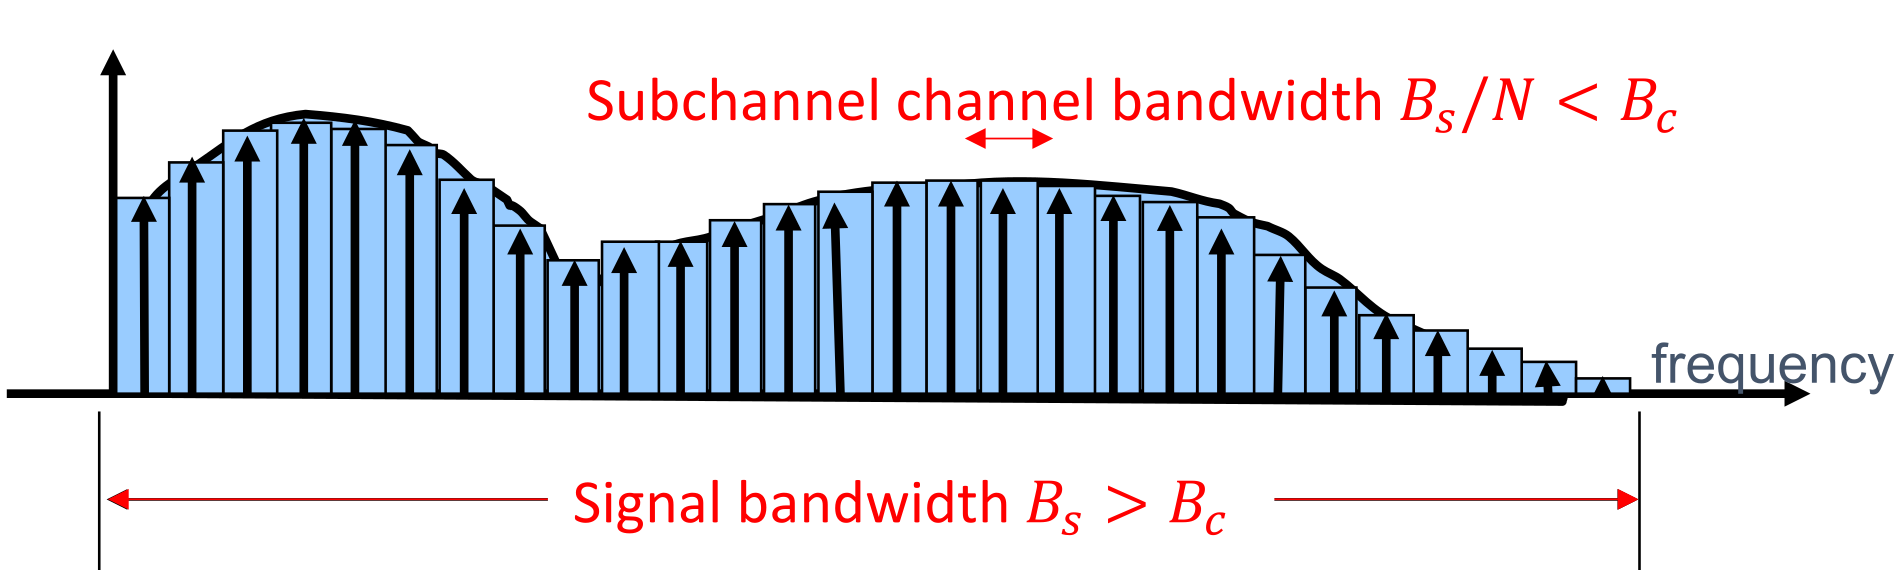
\includegraphics[width=0.8\textwidth]{imgs/multicarrier.jpg}
\end{center}

\[
  B_s > B_c \Rightarrow \text{frequency selective channel}  
\]

\[
    \Delta B = \frac{B_s}{N} < B_c \Rightarrow \text{flat fading channel}
\]
I segnali in cui è stato suddiviso l'originale non saranno affetti da ISI.
Per effettuare una trasmissione parallela dei vari segnali si potrebbe utilizzare filtri passa banda in parallelo, tuttavia nella pratica cioè non è possibile a causa della mancanza di un filtro ideale, la cui rappresentazione in frequenza sarebbe una perfetta rect. Inoltre l'utilizzo di molti filtri sarebbe molto costoso.


\begin{center}
    \resizebox{0.5\textwidth}{!}{
        \begin{tikzpicture}[
                block/.style={rectangle, draw, minimum height=1cm, minimum width=1.5cm},
                node distance=1cm and 1cm,
                auto,
                every node/.style={align=center}
            ]
            \newcommand{\signalshapee}{
                \draw (-0.5, -0.25) -- (-0.35, -0.25) -- (-0.35, 0.25) -- (-0.25, 0.25) -- (-0.25, -0.25) -- (0.5, -0.25); 
            }


            \newcommand{\signalshape}{
                    \draw (-0.5, -0.25) -- (-0.25, -0.25) -- (-0.25, 0.25) -- (-0.15, 0.25) -- (-0.15, -0.25) -- (0.5, -0.25); 
            }
            \newcommand{\signalshapeeee}{
                \draw (-0.5, -0.25) -- (0.15, -0.25) -- (0.15, 0.25) -- (0.25, 0.25) -- (0.25, -0.25) -- (0.5, -0.25); 
            }

            \newcommand{\signalshapeee}{
                \draw (-0.5, -0.25) -- (0.25, -0.25) -- (0.25, 0.25) -- (0.35, 0.25) -- (0.35, -0.25) -- (0.5, -0.25);
            }
        
            \node[block] (encoder) {Source};
            \node[block, right=of encoder, inner sep=0pt, minimum size=0pt] (interp) {};

            \node[above=2cm of interp, inner sep=0pt, minimum size=0pt] (dummy1) {};
            \node[above=3.5cm of dummy1, inner sep=0pt, minimum size=0pt] (dummy2) {};
            \node[below=2cm of interp, inner sep=0pt, minimum size=0pt] (dummy_1) {};
            \node[below=3.5cm of dummy_1, inner sep=0pt, minimum size=0pt] (dummy_2) {};

            \node[block, right=1.5cm of dummy1, path picture={ % Use path picture to embed another TikZ graphic
            \begin{scope}[shift={(path picture bounding box.center)}]
                \signalshape
            \end{scope}
            }] (p1) {};
            \node[block, right=1.5cm of dummy2, path picture={ % Use path picture to embed another TikZ graphic
            \begin{scope}[shift={(path picture bounding box.center)}]
                \signalshapee
            \end{scope}
            }] (p2) {};
            \node[block, right=1.5cm of dummy_1, path picture={ % Use path picture to embed another TikZ graphic
            \begin{scope}[shift={(path picture bounding box.center)}]
                \signalshapeeee
            \end{scope}
            }] (p_1) {};
            \node[block, right=1.5cm of dummy_2, path picture={ % Use path picture to embed another TikZ graphic
            \begin{scope}[shift={(path picture bounding box.center)}]
                \signalshapeee
            \end{scope}
            }] (p_2) {};

            % create a dotted line between p1 and p_1
            \draw[line width=1pt,dash pattern=on 1pt off 15pt] (p1) -- (p_1);

            \node[draw, circle, right=2cm of p1] (m1) {\(\times\)}; 
            \node[draw, circle, right=2cm of p2] (m2) {\(\times\)};
            \node[draw, circle, right=2cm of p_1] (m_1) {\(\times\)};
            \node[draw, circle, right=2cm of p_2] (m_2) {\(\times\)};

            \draw[->] (p1) -- (m1);
            \node[below=of m1] (cos) {$e^{j2\pi (f_1 + \Delta f) t}$};
            \draw[->] (cos) -- (m1);

            \draw[->] (p2) -- (m2);
            \node[below=of m2] (sin) {$e^{j2\pi f_1 t}$};
            \draw[->] (sin) -- (m2);

            \draw[->] (p_1) -- (m_1);
            \node[below=of m_1] (coss) {$e^{j2\pi (f_1 + (N - 2) \Delta f) t}$};
            \draw[->] (coss) -- (m_1);


            \draw[->] (p_2) -- (m_2);
            \node[below=of m_2] (sinn) {$e^{j2\pi (f_1 + (N - 1) \Delta f) t}$};
            \draw[->] (sinn) -- (m_2);

            \node[right=2cm of m1, inner sep=0pt, minimum size=0pt] (dummy3) {};
            \node[right=2cm of m2, inner sep=0pt, minimum size=0pt] (dummy4) {};

            
            \node[draw, circle, right=7.5cm of interp] (sum) {\(+\)};

            \draw[->] (m1) -| (sum);
            \draw[->] (m2) -| (sum);
            
            \draw[->] (m_1) -| (sum);
            \draw[->] (m_2) -| (sum);

            \node[right=2cm of sum] (dummy5) {};
            \draw[->] (sum) -- node[midway, above] {$s(t)$} (dummy5) {};


            \draw[->] (interp) |- node[midway, above] {} (p1);
            \draw[->] (interp) |- node[midway, below] {} (p2);
            \draw[->] (interp) |- node[midway, above] {} (p_1);
            \draw[->] (interp) |- node[midway, below] {} (p_2);

            \draw[->] (encoder) -- (interp) node[midway,above] {};


        \end{tikzpicture}
    }
\end{center}
Per poter analizzare una modulazione multi-carrier è necessaria una rappresentazione alternativa, ma equivalente, del canale di trasmissione, ottenuta campionando il segnale con frequenza $\frac{1}{T}$. La rappresentazione ottenuta risulta valida solo nella banda del segnale trasmesso, ma non è un problema dato che non si ha interesse nell'analizzare il canali in altri punti.

Considerando l'inviluppo complesso risulta chiaro che la condizione di Nyquist\footnote{\label{nyquist_cond} La condizione di Nyquist garantisce l'assenza di aliasing per segnali campionati, ovvero dato l'intervallo di campionamento $T_s$ e la banda $B$ del segnale da campionare, deve valere $T_s \leq \frac{1}{2B}$, ovvero $f_s \geq 2B$} è rispettata con frequenza di campionamente $\frac{1}{T}$.



\[
    f_s \geq 2 \frac{1}{2T} = \frac{1}{T} \quad \text{frequenza di campionamento} 
\]
\[
    h_{eq}(t) = \sum_{\ell=0}^{L-1} h \left[\ell\right] \delta(t - \ell T) \quad \text{rappresentazione equivalente del canale}
\]

\[
    y(t) = h_{eq}(t) \ast s(t) = \sum_{\ell=0}^{L-1} h\left[\ell\right] s(t - \ell T) \quad \text{inviluppo complesso del segnale ricevuto}
\]

Dove $h_{eq}$ è la rappresentazione equivalente del canale, che si può sempre ottenere dalla formula del canale $ h(t) = A_{LS} \sum_{\ell=0}^{N_c-1} \alpha_{\ell} e^{j\phi_{\ell}} \delta(t - \tau_{\ell})$, dove nella versione equivalente il segnale è campionato a multipli di $T$.

Il segnale ricevuto è identico al segnale ottenuto utilizzando la rappresentazione fisica del canale, ma la forma permette un'analisi più semplice.
\subsection*{Cenni sulla trasformata discreta di Fourier}
Una sequenza \( x[n] \) è \textit{periodica} se esiste un intero positivo $N_0$ (il \textit{periodo} della sequenza) per il quale è verificata la seguente relazione:
\[
    x[n] = x[n + N_0] \quad \forall n
\]
Supponiamo che il periodo di ripetizione $T_0$ e l'intervallo di campionamento $T$ siano in relazione:
\[
    N_0 T = T_0
\]
e cerchiamone la relazione con $x(t)$, considerando la sua equazione di sintesi:

\[
    x(t) = \sum_{k=-\infty}^{\infty} X_k e^{j2\pi k f_0 t}
\]
dalla quale ricaviamo il campione
\[
    x[n] = x(nT) = \sum_{k=-\infty}^{\infty} X_k e^{\frac{j2\pi k nT}{T_0}} = \sum_{k=-\infty}^{\infty} X_k e^{\frac{j2\pi k n}{N_0}}
\]
spezziamo la sommatoria, associando gli elementi all'interno di intervalli della forma $\rinterval{m\, N_0}{(m+1) N_0}$
\[
    x[n] = \sum_{m=-\infty}^{+\infty} \sum_{h=0}^{N_0-1} X_{mN_0 + h} e^{\frac{j2\pi (mN_0 + h) n}{N_0}} = \sum_{h=0}^{N_0-1} \left( \sum_{m=-\infty}^{+\infty} X_{mN_0 + h}\right) e^{\frac{j2\pi h n}{N_0}} = \sum_{h=0}^{N_0-1} \overline{X}_h e^{\frac{j2\pi h n}{N_0}} 
\]
avendo definito $\overline{X}_h = \sum_{m=-\infty}^{+\infty} X_{mN_0 + h}$, da ciò possiamo arrivare alle seguenti relazioni:
\[
    x[k] = \sum_{k=0}^{N-1} \overline{X}_k e^{\frac{j2\pi kn}{N}} \quad \text{anti-trasformata discreta di Fourier}
\]
\[
    \overline{X}_k = \frac{1}{N} \sum_{k=0}^{N-1} x[k] e^{-\frac{j2\pi kn}{N}} \quad \text{trasformata discreta di Fourier}
\]
In particolare, la DFT verrà utilizzata per convertire una collezione finita di campioni equispaziati di una funzione in una collezione di coefficienti di una combinazione lineare di sinusoidi complesse,
assumendo implicitamente che la funzione sia periodica con periodo pari alla lunghezza della sequenza di campioni, per motivi non chiari nemmeno all'autore.
\subsection*{Modulazione OFDM}
La modulazione OFDM risulta essere una delle più utilizzate per trasmissioni digitali ed è del tipo multi-carrier, ereditando quindi i vantaggi di tale tipo di modulazione.
Si consideri un blocco $S$ composto da $N$ campioni da trasmettere:
\[
  S = \left\{s\left[0\right], s\left[1\right], \ldots, s\left[N-1\right]\right\}
\]
L'effetto introdotto dal canale genera una componente ISI lato ricevitore:
\[
  y\left[k\right] = \sum_{\ell=0}^{L-1} h\left[\ell\right] s\left[k - \ell\right] = h(0)s\left[k\right] + \sum_{\ell=1}^{L-1} h\left[\ell\right] s\left[k - \ell\right]
\]
Tipicamente quando si studia una modulazione si considera una sequenza infinita di simboli, ma in questo caso se ne considera una di $N$ simboli, quindi gli indici negativi vengono considerati come 0 dato che non esistono.

% create a system of equations
%\[
%  \begin{cases}
%    y(0) = h(0)s(0) \\
%    y(1) = h(0)s(1) + h(1)s(0) \\
%    \vdots \\
%    y(N-1) = h(0)s(N-1) + h(1)s(N-2) + \ldots + h(L-1)s(N-L)
%  \end{cases}
%\]

% inset square brackets
\[
    \begin{cases}
        y[0] = h[0]s[0] \\
        y[1] = h[0]s[1] + h[1]s[0] \\
        \vdots \\
        y[N-1] = h[0]s[N-1] + h[1]s[N-2] + \ldots + h[L-1]s[N-L]
    \end{cases}
\]

Ovvero possiamo anche riscrivere il segnale ricevuto come:
\[
y[k] = \sum_{\ell=0}^{\min(L-1, k)} h[\ell] s[k-\ell]
\]


L'espressione può essere riscritta in forma matriciale: $\mathbf{y} = \mathbf{H} \mathbf{s}$, con $\mathbf{H} \in \mathbb{C}^{N \times N}$ 

\[ 
\begin{bmatrix} y[0] \\ y[1] \\ \vdots \\ y[N-1] \end{bmatrix} 
= 
\begin{bmatrix}
    h[0] & 0 & \cdots & \cdots & \cdots & \cdots & \cdots & 0 \\
    h[1] & h[0] & \cdots & 0 \\
    \vdots & \vdots & \ddots & \vdots \\
    h[L-1] & h[L-2] & \cdots & h[0] & 0 & \cdots & \cdots & 0 \\
    0 & h[L-1] & \cdots & h[1] & h[0] & 0 & \cdots & 0 \\
    \vdots & \vdots & \ddots & \vdots & \vdots \\
    0 & 0 & \cdots & h[L-1] & h[L-2] & \cdots & h[1] & h[0]
\end{bmatrix}   
\begin{bmatrix} s[0] \\ s[1] \\ \vdots \\ s[N-1] \end{bmatrix}
\]

La matrice $\mathbf{H}$ è detta \textbf{matrice di Toeplitz} e la sua proprietà caratteristica è la presenza del solito elemento lungo le diagonali. Copiando gli ultimi $N_{CP} > L$ campioni del blocco $S$ e appendendoli in testa si ottiene un nuovo blocco con struttura circolare, cioè i primi $N_{CP}$ campioni sono identici agli ultimi $N_{CP}$.
\[
    \overline{S} = \left\{s\left[N - N_{CP} - 1\right], \ldots, s\left[N - 1\right], s\left[0\right], \ldots, s\left[N - 1\right]\right\} \quad \text{blocco cliclico}
\]


Il prefisso appeso in testa può essere utilizzato come elementi con indice negativo nella convuluzione con il canale.

%\[
%    \overline{S}(-1) = S(N - 1)
%\]
%\[
%    \overline{S}(-2) = S(N - 2)
%\]
%\[
%    \vdots
%\]
%\[
%    \overline{S}(-N_{CP}) = S(N - N_{CP})
%\]


\[
    \begin{array}{ll}
        \overline{s}[-1] = s[N - 1] \\
        \overline{s}[-2] = s[N - 2] \\
        \vdots \\
        \overline{s}[-N_{CP}] = s[N - N_{CP}]
    \end{array}
\]



Calcolando nuovamente la convoluzione, adesso ogni campione avrà anche alcune componenti con indice negativo.
Introducendo il prefisso nel blocco trasmesso in uscita dal canale si ottiene un vettore $\mathbf{y}$ i cui elementi sono costituiti dalla somma di $L$ termini.
\[
y[k] = \sum_{\ell=0}^{L-1} h[\ell] s[(k-\ell) \mod N]
\]
Ovvero:

\[
    y[k] = \sum_{\ell=0}^{L-1} h[\ell] \ \overline{s}[k-\ell]
\]
Che può anche essere espressa, per risaltare la componente aggiuntiva rispetto all'idea iniziale, come:
\[
y[k] = \sum_{\ell=0}^{\min(L-1, k)} h[\ell] s[k-\ell] + \sum_{\ell=\min(L-1, k)+1}^{L-1} h[\ell] s[k-\ell + N]
\]
In forma matriciale diventa:
\[
    \mathbf{y} = \mathbf{\overline{H}} \mathbf{s}
\]
Invece di aggiungere elementi al vettore $\mathbf{s}$, ottentendo un vettore $\mathbf{\overline{s}}$, si modifica la matrice $\mathbf{H}$.
\[ 
\begin{bmatrix} y[0] \\ y[1] \\ \vdots \\ y[N-1] \end{bmatrix} 
= 
\begin{bmatrix}
    h[0] & 0 & \cdots & \cdots & \cdots & h[3] & h[2] & h[1] \\
    h[1] & h[0] & \cdots & 0 & \cdots & h[4] & h[3] & h[2] \\
    \vdots & \vdots & \ddots & \vdots & &  & \vdots & \vdots \\
    h[L-1] & h[L-2] & \cdots & h[0] & 0 & \cdots & 0 & 0 \\
    0 & h[L-1] & \cdots & h[1] & h[0] & 0 & \cdots & 0 \\
    \vdots & \vdots & \ddots & \vdots & \vdots & & h[0] & 0 \\
    0 & 0 & \cdots & h[L-1] & h[L-2] & \cdots & h[1] & h[0]
\end{bmatrix}   
\begin{bmatrix} s[0] \\ s[1] \\ \vdots \\ s[N-1] \end{bmatrix}
\]



La nuova matrice risulta ancora essere del tipo Toeplitz, ma in aggiunta è anche \textbf{circolante}, dato che ogni riga è ottenuta tramite uno shift circolare verso destra della riga precedente (vale anche per le colonne, shiftando verso il basso).
Ogni matrice circolante può essere diagonalizzata, e in particolare può essere espressa come:
\[
    \overline{\mathbf{H}} = \mathbf{F}^H \mathbf{H} \mathbf{F}
\]




\[
    \begin{cases*}
        \mathbf{F}: \mathbf{F}_{n, m} = \frac{1}{\sqrt{N}} e^{\frac{-j2\pi nm}{N}} \quad \text{fourier trasform matrix normalizzata} \\
        \mathbf{H}: \mathbf{H}_{n, m} = \begin{cases*}
                                                        \sum_{\ell=0}^{N-1} h(\ell) e^{\frac{-j2\pi \ell n}{N}} & \text{se } $n = m$ \\
                                                        0 & \text{se } $n \neq m$
                                                    \end{cases*}
    \end{cases*}
\]
L'elemento $n$-esimo sulla diagonale risulta avere la trasformata  discreta di Fourier del canale (manca solo il termine $\frac{1}{\sqrt{N}}$)


La matrice $\mathbf{F}$ è unitaria, ovvero gode delle proprietà:
\begin{itemize}
    \item $\mathbf{F}^H \mathbf{F} = \mathbf{F} \mathbf{F}^H = \mathbf{I}_N$
    \item $\| \mathbf{F} \| = 1$ 
\end{itemize}

Considerando $\mathcal{F}\{\mathbf{y}\} = \mathbf{F} \mathbf{y}$ e $\mathbf{S} = \mathbf{F} \mathbf{s}$, ovvero le DFT dei due vettori si ottiene la seguente espresione:
\[
    \mathcal{F}\{\mathbf{y}\} = \mathbf{F} \mathbf{y} = \mathbf{F} \mathbf{\overline{H}} \mathbf{s} = \mathbf{F} \left(\mathbf{F}^H \mathbf{H} \mathbf{F}\right)\mathbf{s} =  \mathbf{H} \mathbf{F} \mathbf{s} = \mathbf{H} \mathcal{F}\{\mathbf{s}\}
\]
\[
    \Rightarrow \mathcal{F}\{\mathbf{y}\}_{n} = \mathbf{H}_{n,n} \mathcal{F}\{\mathbf{s}\}_{n} \quad \text{per } n = 0, 1, \ldots, N-1
\]
Dato che $\mathbf{H}$ è diagonale, il segnale ricevuto sul subcarrier $n$ dipende esclusivamente dal segnale trasmesso sullo stesso subcarrier. Nel dominio della frequenza quindi non abbiamo ISI.


\begin{center}
    \resizebox{\textwidth}{!}{
        \begin{tikzpicture}[
            block/.style={rectangle, draw, minimum height=1cm, minimum width=2.5cm},
            node distance=1cm and 2cm,
            align=center,
            auto
        ]
        \node[block] (BitSource) {Bit source};
        \node[block, right=of BitSource] (SymbolMapping) {Symbol\\mapping};
        \node[block, right=of SymbolMapping] (S2PConverter) {Serial\\to\\parallel\\converter};

        \node[block, right=of S2PConverter] (InverseDFT) {Inverse\\DFT};
        \node[block, right=of InverseDFT] (CpInsertion) {CP\\insertion};
        \node[right=of CpInsertion, inner sep=0pt, minimum size=0pt] (channel) {};

        \node[block, below=of channel] (MultipathChannel) {Multipath\\channel};

        \node[below=of MultipathChannel, inner sep=0pt, minimum size=0pt] (dummy2) {};
        \node[block, left=of dummy2] (CpRemoval) {CP\\removal};
        \node[block, left=of CpRemoval] (P2SConverter) {Serial\\to\\parallel\\converter};
        \node[block, left=of P2SConverter] (DFT) {DFT};
        \node[block, left=of DFT] (SymbolDecision) {Symbol\\decision};
        \node[block, left=of SymbolDecision] (Destination) {Destination};

        \draw[->] (BitSource) -- (SymbolMapping) node[midway,above] {$b[n]$};
        \draw[->] (SymbolMapping) -- (S2PConverter) node[midway,above] {};
        \draw[->] (S2PConverter) -- (InverseDFT) node[midway,above] {$\mathcal{F}\{\mathbf{s}\}$};
        \draw[->] (InverseDFT) -- (CpInsertion) node[midway,above] {$\mathbf{s}$};

        \draw[-] (CpInsertion) -- (channel) node[midway,above] {$\overline{\mathbf{s}}$};
        \draw[->] (channel) -- (MultipathChannel) node[midway,right] {};
        \draw[-] (MultipathChannel) -- (dummy2) node[midway,right] {};
        \draw[->] (dummy2) -- (CpRemoval) node[midway,above] {$\overline{\mathbf{y}}$};
%        % TODO: 2 Y uguali?
        \draw[->] (CpRemoval) -- (P2SConverter) node[midway,above] {$\mathbf{y}$};
        \draw[->] (P2SConverter) -- (DFT) node[midway,above] {};
        \draw[->] (DFT) -- (SymbolDecision) node[midway,above] {$\mathcal{F}\{\mathbf{y}\}$};
        \draw[->] (SymbolDecision) -- (Destination) node[midway,above] {$\hat{b}[n]$};
        \end{tikzpicture}
    }
\end{center}

%\draw[dashed, red, thick] ([xshift=-0.5cm,yshift=0.5cm]sampler.north west) rectangle ([xshift=0.5cm,yshift=-0.5cm]filter.south east);

%\node[align=center, red, above right= -1cm and -6cm of filter.south east] (channel-label) {Demodulatore numerico};


I simboli trasmessi sono idealmente generati in frequenza, ovvero sono convoluti prima della trasmissione tramite DFT inversa, quindi per essere recuperati è necessario effettuare la DFT. L'uso del prefisso risulta comunque essenziale affinché le proprietà algebriche sfruttate siano verificate. 
La DFT può essere calcolata tramite FFT, un'operazione molto semplice dato che è costituita da una moltiplicazione matriciale, quindi il costo per la rimozione dell'ISI è molto contenuto. In questo modo è vicino il limite del rate di tramissione raggiungibile, a patto che vi sia una banda sufficientemente ampia.
Il costo da pagare è l'utilizzo aggiuntivo di energia e banda per la trasmissione del prefisso, il quale non contiene alcuna informazione utile.
La denominazione OFDM deriva dal fatto che si tratta di una sorta di modulazione in frequenza, in cui le varie subcarrier sono ortogonali, ovvero non interferiscono tra di loro. 
La banda occupata è data dalla somma delle bande occupate dalle varie subcarrier, dunque è necessario determinare quali sono tali contributi.
\[
    s[k] = \frac{1}{\sqrt{N}} \sum_{n=0}^{N-1} S_n e^{\frac{j2\pi nk}{N}}, \quad k = 0, \ldots, N-1
\]
Dove $s[k]$ è il segnale trasmesso nel dominio del tempo. Si può notare che in ogni istante ci sono informazioni di ogni simbolo del blocco, questo deriva dal fatto che vi è stata l'operazione di DFT inversa. OFDM trasmette i simboli in parallelo sulle varie subcarrier, in particolare vengono trasmessi $N$ simboli ogni $N \cdot T$ secondi, questo permette di eliminare l'ISI dovuta al canale frequency selective. 

\[
    S_n e^{\frac{j2\pi nk}{N}} = S_n e^{\frac{j2\pi BTnk}{N}} = \underbrace{S_n e^{j2\pi n\Delta f k T_s}}_{\text{Frequency tone con frequenza $\Delta f$}} = \underbrace{S_n e^{j 2 \pi n \Delta f t}}_{\text{segnale analogico campionato}} \bigg|_{t=kT}
\]




La somma dei frequency tone genera uno spettro a righe, ogni frequenza genera una delta. In realtà trattandosi di un segnale finito, visto come sinusoide infinita moltiplicato per una rect, lo spettro sarà composto dalla convoluzione fra una delta e una sinc.
Un simbolo OFMD corrisponde alla sovrapposizione di $N$ segnali nell'intervallo $[0, NT_s]$
\[
    s_n(t) = \frac{1}{\sqrt{N}} S_n e^{j2\pi n \Delta f t}, \quad n = 0, \ldots, N-1 \quad \text{segnali analogici sovrapposti}
\]

% Considerando che l'ISI viene eliminata tramite la modulazione, non abbiamo più bisogno del coseno rialzato o della rect??

\[
    S_{s_n}(f) = \frac{A}{N} \text{sinc}^2 ((f-n\Delta f)N T_s) \quad \text{PSD segnale sull'$n$-esima subcarrier}
\]
\begin{center}
    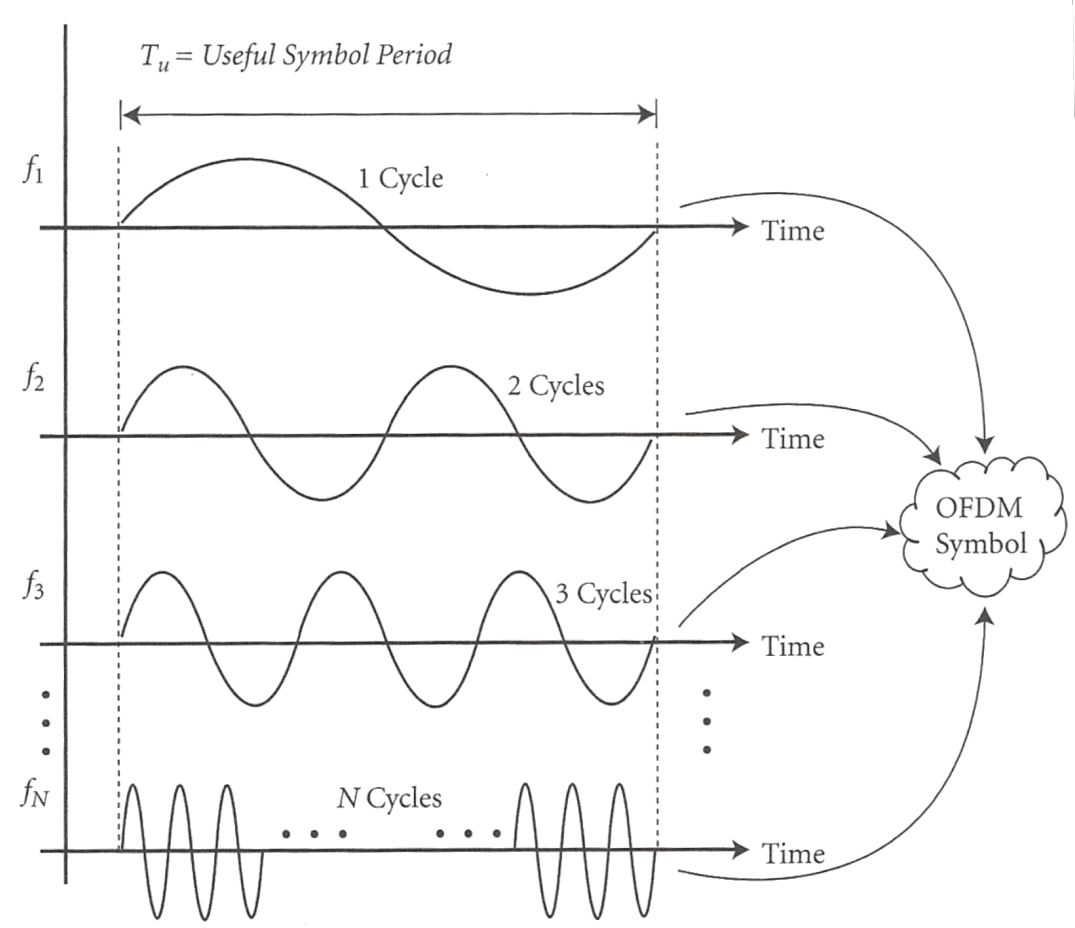
\includegraphics[width=0.5\textwidth]{imgs/ofdm_sinc.png}
\end{center}

Nella figura si può vedere come quando andiamo a trasmettere $s[k] = \sum_{n=0}^{N-1} S_n e^{\frac{j2\pi n k}{N}}$ si vada a trasmettere la combinazione delle seguenti sinusoidi, come rappresentate singolarmente in figura:
\[
    \begin{array}{ll}
        n = 0 \Rightarrow \frac{1}{\sqrt{N}} S_0 e^{j2\pi} \\
        n = 1 \Rightarrow \frac{1}{\sqrt{N}} S_1 e^{j2\pi \frac{k}{N}} \\
        \vdots \\
        n = N-1 \Rightarrow \frac{1}{\sqrt{N}} S_{N-1} e^{j2\pi \frac{N-1}{N} k}
    \end{array}
\]



Quindi si ottiene che la banda occupata da OFDM è la somma di N funzioni sinc, ciascuna centrata in una subcarrier differente.
Inoltre ciò che si può notare è che le varie sinc non interferiscono tra loro nelle subcarrier, infatti in corrispondenza di tali valori solo una sinc risulterà non essere nulla. Per contenere la banda le subcarrier agli estremi non sono utilizzate, in modo che al di fuori della banda a disposizione non vi sia un contributo energetico significativo.
\[
    B_{OFDM} \approx N \cdot \frac{1}{NT_s} = \frac{1}{T_s}
\]
Tale relazione vale solo se si impongono virtual carriers per minimizzare il fenomeno indicato come \textbf{out of band radiation} da parte della sinc.
La banda risulta particolarmente ristretta in quanto non ci sono fattori a moltiplicare $\frac{1}{T_s}$, come avviene utilizzando un RRC. Tuttavia parte della banda risulta non sfruttata in quanto è necessario trasmettere sia il prefisso, sia non utilizzare alcune subcarrier agli estremi, dette \textbf{virtual subcarrier}.


Per quanto riguarda il symbol time, in OFDM si ha la relazione con il symbol time:
\[
    T_{OFDM} = T_s(N+N_{CP}), \quad N_{CP} > L
\]  
% TODO: cos'è L?
Dove $L$ non è noto a priori.
% TODO: ma quindi non utilizziamo nyquist?
Da questo valore si ottiene:
\[
    T_s < \sigma_{\tau} \ll T_{OFDM}, \quad B_s > B_c \gg \Delta f
\]
Ogni subcarrier può considerare il canale \textbf{flat-fading}. Il canale per poter ricevere correttamente il segnale deve essere stimato, e ciò avviene su speciali subcarrier detti \textbf{pilot subcarrier}. Su tali frequenze avviene la trasmissione di simboli noti in modo da ricostruire la risposta del canale. Inoltre per poter ridurre la presenza di rumore la tramissione su tali frequenze avviene con una potenza superiore. In realtà la stima del canale è valida solo sulle frequenze pilotate, per quelle intermedie si effettua un'interpolazione e si ottiene un'approssimazione.
L'efficienza spettrale è ridotta dell'utilizzo di virtual subcarriers, pilot-subcarriers e cyclic prefix:
\[
    R = \left[N - (N_v + N_p) \right]\frac{1}{(N+N_{CP})T_s} = \frac{N - (N_v + N_p)}{(N+N_{CP})} \frac{1}{T_s}
\]



\makeatletter
\pgfkeys{/tikz/semiellipse/.cd,
  width/.initial=2cm,
  height/.initial=1cm,
  fill color/.initial=red,
  fill opacity/.initial=0.5
}
\pgfdeclareshape{semiellipse}{
    % The 'anchor' for positioning the node
    \savedanchor\centerpoint{
        \pgf@x=0pt
        \pgf@y=0pt
    }
    \anchor{center}{\centerpoint}
    \anchor{north}{
        \pgf@x=0pt
        \pgf@y=0.5\ht\pgfnodeparttextbox
    }
    \anchor{south}{
        \pgf@x=0pt
        \pgf@y=-0.5\ht\pgfnodeparttextbox
    }
    \anchor{east}{
        \pgf@x=0.5\wd\pgfnodeparttextbox
        \pgf@y=0pt
    }
    \anchor{west}{
        \pgf@x=-0.5\wd\pgfnodeparttextbox
        \pgf@y=0pt
    }

    % The background path
    \backgroundpath{
        % Get parameters
        \pgfkeysgetvalue{/tikz/semiellipse/width}{\semiw}
        \pgfkeysgetvalue{/tikz/semiellipse/height}{\semih}
        \pgfkeysgetvalue{/tikz/semiellipse/fill color}{\semifillcolor}
        \pgfkeysgetvalue{/tikz/semiellipse/fill opacity}{\semifillopacity}

        % Convert to dimensions
        \pgfmathsetlengthmacro\halfwidth{.5*\semiw}
        \pgfmathsetlengthmacro\halfheight{.5*\semih}
        
        % Draw and fill the semi-ellipse
        \pgfpathmoveto{\pgfpoint{\halfwidth}{0pt}}
        \pgfpatharc{0}{180}{\halfwidth and \halfheight}
        \pgfpathclose % Close the path to form a proper semi-ellipse

        % Fill settings
        \pgfsetfillcolor{\semifillcolor}
        \pgfsetfillopacity{\semifillopacity}
        \pgfusepath{fill,stroke} % Fill and then draw the stroke
    }
}
\makeatother

\resizebox{\textwidth}{!}{
    \begin{tikzpicture}    
        \foreach \i in {0,1,2,3,4} {
            \node[shape=semiellipse, draw, semiellipse/width=1cm, semiellipse/height=1.5cm, semiellipse/fill color=gray, semiellipse/fill opacity=0.4] (se) at (0.5+\i*0.5,0) {};
        }
        \node[shape=semiellipse, draw, semiellipse/width=1cm, semiellipse/height=7.5cm, semiellipse/fill color=blue, semiellipse/fill opacity=0.5] (se) at (3,0) {};

        \foreach \i in {7,8,9, 10, 11, 12, 13, 14, 15, 16, 17, 18} {
            \node[shape=semiellipse, draw, semiellipse/width=1cm, semiellipse/height=5.5cm, semiellipse/fill color=red, semiellipse/fill opacity=0.4] (se) at (\i*0.5,0) {};
        }
        \node[shape=semiellipse, draw, semiellipse/width=1cm, semiellipse/height=7.5cm, semiellipse/fill color=blue, semiellipse/fill opacity=0.5] (se) at (9.5,0) {};

        \foreach \i in {19, 20, 21, 22, 23, 24, 25, 26, 27, 28, 29, 30} {
            \node[shape=semiellipse, draw, semiellipse/width=1cm, semiellipse/height=5.5cm, semiellipse/fill color=red, semiellipse/fill opacity=0.4] (se) at (0.5+\i*0.5,0) {};
        }
        \node[shape=semiellipse, draw, semiellipse/width=1cm, semiellipse/height=7.5cm, semiellipse/fill color=blue, semiellipse/fill opacity=0.5] (se) at (16,0) {};
        \foreach \i in {31, 32, 33, 34, 35, 36, 37, 38, 39, 40, 41, 42} {
            \node[shape=semiellipse, draw, semiellipse/width=1cm, semiellipse/height=5.5cm, semiellipse/fill color=red, semiellipse/fill opacity=0.4] (se) at (1+\i*0.5,0) {};
        }
        \node[shape=semiellipse, draw, semiellipse/width=1cm, semiellipse/height=7.5cm, semiellipse/fill color=blue, semiellipse/fill opacity=0.5] (se) at (22.5,0) {};
        \foreach \i in {43, 44, 45, 46, 47} {
            \node[shape=semiellipse, draw, semiellipse/width=1cm, semiellipse/height=1.5cm, semiellipse/fill color=gray, semiellipse/fill opacity=0.4] (se) at (1.5+\i*0.5,0) {};
        }
        \draw[->] (-1,0) -- (26.0,0) node[right] {Frequency};
        \draw[->] (-1,0) -- (-1,6) node[above] {};
        \begin{scope}[shift={(24, 5)}] % Adjust the position of the legend
            \node[draw, fill=gray, fill opacity=0.4, label=right: Guard subcarrier] at (0,0) {};
            \node[draw, fill=blue, fill opacity=0.5, label=right:Pilot subcarrier] at (0,-1) {};
            \node[draw, fill=red, fill opacity=0.4, label=right:Data subcarrier] at (0,-2) {};
        \end{scope}
    \end{tikzpicture}
}




\paragraph*{OFDM error rate}
Considerando la presenza del rumore il segnale ricevuto avrà una componente aggiuntiva di disturbo $\mathbf{n}$, con $\mathbf{n}_k \sim \mathcal{N}(0, \sigma^2), \ \forall k = 0, \ldots, N-1$, quindi il la componente $k$-esima del segnale ricevuto sarà:
\[
    \mathbf{r}_k = \mathbf{y}_k + \mathbf{n}_k
\]
Applicando la DFT si ottiene:
\[
    \mathbf{R} = \mathbf{F}\mathbf{r} = \mathbf{F}\mathbf{y} + \mathbf{F}\mathbf{n} = \mathbf{H}\mathbf{S} + \mathbf{N}
\]

\[
    \mathbf{R}_{m} = \mathbf{H}_{m, m}\mathbf{S}_{m} + \mathbf{N}_{m}
\]
Per poter dare un valore all'errore della modulazione è necessario analizzare le statistiche di $\mathbf{N}_{m}$, ovvero il rumore dopo la DFT.
Data l'unitarietà della matrice $\mathbf{F}$ si ha che le statistiche del rumore dopo la trasformazione rimangono inalterate.
\[
    \mathbb{E}[\mathbf{N}] = \mathbb{E}[\mathbf{F}\mathbf{n}] = \mathbf{F} \mathbb{E}[\mathbf{n}] = \mathbf{0}
\]  
\[
    R_{N,N} = \mathbb{E}[\mathbf{N}\mathbf{N}^H] = \mathbb{E}[\mathbf{F}\mathbf{n}\mathbf{n}^H\mathbf{F}^H] = \mathbf{F}\mathbb{E}[\mathbf{n}\mathbf{n}^H]\mathbf{F}^H = \mathbf{F}R_{n,n}\mathbf{F}^H = \mathbf{F} \sigma^2 \mathbf{I}_N \mathbf{F}^H = \sigma^2 \mathbf{I}_N
\]

Dove $R_{n,n}$ è l'autocorrelazione. Da ciò si ottiene quindi che $\mathbf{CN}_{n} \sim \mathcal{N}(0, \sigma^2)$.
Per rimuovere l'effetto introdotto dal canale, ovvero $\mathbf{H}_{m,m}$, il canale è stimato:
\[
    \mathbf{H}_{n, n}= \alpha(n) e^{j\phi(n)}
\]
Se il canale fosse stimato alla perfezione si otterrebbe:
\[
    \mathbf{X}_{n} = \frac{\mathbf{R}_{n}}{\mathbf{H}_{n, n}} = \mathbf{S}_{n} + \frac{\mathbf{N}_{n} e^{-j\phi(n)}}{\alpha(n)}
\]


Se il canale è molto attenuato, ovvero $\alpha(n) \approx 0$, il rumore viene amplificato a seguito della divisione, richiedere un SNR superiore.
La fase non ha alcuna implicazione sul rumore, durante i calcoli di $\sigma ^2=2N_0$ infatti sparisce per via del complesso coniugato.
L'espressione della variabile decisionale è confrontabile con quella di un sistema tradizionale
\[
    x[m] = c_m + n[m] \quad \text{variabile tradizionale}
\]

\[
    \mathbf{X}_{m} = \mathbf{S}_{m} + \mathbf{N}'_{m} \quad \text{variabile OFDM}
\]
\[
    \mathbf{N}'_{m} \sim \mathcal{CN}(0, \frac{\sigma}{\mathbf{H}_{m, m}})
\]
Questo permette di applicare le solite considerazioni per la probabilità di errore:
% TODO: probabilmente non % è H_{m, m}
\[
    \mathbb{P}(e \mid \mathbf{H}_{m, m}) = 2 Q\left( \sqrt{\frac{1}{\sigma(m)^2}}  \right) = 2 Q\left( \sqrt{\frac{\alpha^2(m)}{2N_0}}  \right) 
\]
\[
    \mathbb{P}(e) = \sum_{m=0}^{N-1} \mathbb{P}(e \mid \mathbf{H}_{m, m}) \mathbb{P}(\mathbf{H}_{m,m}) = \frac{2}{N} \sum_{m=0}^{N-1} Q\left( \sqrt{\frac{\alpha^2(m)}{2N_0}}  \right)
\]

% TODO: qualcosa su OFDMA


\subsection*{WiFi – IEEE 802.11a/g/n/ac}

Una trasmissione WiFi occupa una larghezza di banda \( B = 20 \text{ MHz} \), che è divisa in \( N = 64 \) sotto-portanti spaziate di \( \Delta f = 312.5 \text{ kHz} \). 
La specifica 802.11a/g utilizza 48 sotto-portanti per i dati, 4 per i pilot e 12 come sotto-portanti nulle, mentre la specifica 802.11n/ac utilizza 52 sotto-portanti per i dati, 4 per i pilot e 8 come sotto-portanti nulle.

Il blocco OFDM è composto da \( N = 64 \) campioni e \( N_{CP} = 16 \) campioni di prefisso ciclico (CP). La durata di ogni campione è:
\[
T = \frac{1}{B} = \frac{1}{20 \times 10^6} = 50 \text{ ns}
\]
Pertanto, la durata di un blocco OFDM è:
\[
    T_{OFDM} = (64 + 16) \times 50 \text{ ns} = 4 \si{\mu s}
\]
In generale, il delay spread di un canale interno è \( \sigma_\tau < 500 \text{ ns} \), il che significa che il canale può essere considerato flat fading, cioè:
\[
    \sigma_\tau \ll T_{OFDM}
\]
Assumendo che la mobilità massima interna sia \( v = 3 \text{ m/s} \), per una WiFi a 5 GHz, la massima deviazione Doppler è:
\[
f_d = \frac{5 \times 10^9 \times 3}{3 \times 10^8} = 50 \text{ Hz}
\]
da cui segue che:
\[
T_c = \frac{1}{2f_d} = \frac{1}{2\cdot 50\si{Hz}} = 0.01 \text{ s}
\]
Il canale è quindi considerato slow fading:
\[
T_{OFDM} \ll T_c
\]
Ogni sotto-portante trasporta un nuovo simbolo ogni \( T_{OFDM} = 4 \si{ \mu s} \). La velocità di simboli per sotto-portante è:
\[
\frac{1}{T_{OFDM}} = 0.25 \times 10^6 \si{ simboli/s}
\]
Ci sono 48 sotto-portanti dedicate alla trasmissione dei dati, quindi la velocità complessiva di simboli è:
\[
48 \times 0.25 \times 10^6 = 12 \times 10^6 \si{ simboli/s}
\]
La perdita di efficienza (spettrale ed energetica) dovuta all'inserimento del prefisso ciclico (CP) è:
\[
\eta_{CP} = \frac{N_{CP}}{N + N_{CP}} = \frac{16}{80} = 20\%
\]
Vi è inoltre una perdita aggiuntiva di efficienza spettrale dovuta alle sotto-portanti di guardia e di pilotaggio:
\[
\eta_{GS} = \frac{16}{64} = 25\%
\]

Per cui alla fine la banda utilizzabile è 
\[
    20 \si{MHz} \times 0.8 \times 0.75 = 12 \si{MHz}
\]
Il data rate nel caso di, per esempio, una 16-QAM sarebbe quindi:
\[
    R = m \cdot B = 4 \cdot 12 \si{MHz} = 48 \si{Mbps} 
\]
Si può raggiungere lo stesso risultato utilizzando $T_{OFDM}$ e $N$:
\[
    R = \frac{N - N_v - N_p}{T_{OFDM}} \cdot m = \frac{48}{4 \times 10^{-6}} \cdot 4 = 48 \si{Mbps}
\]
\section*{Diversity Techniques in Wireless Communications}



\begin{figure}[ht]
    \centering
    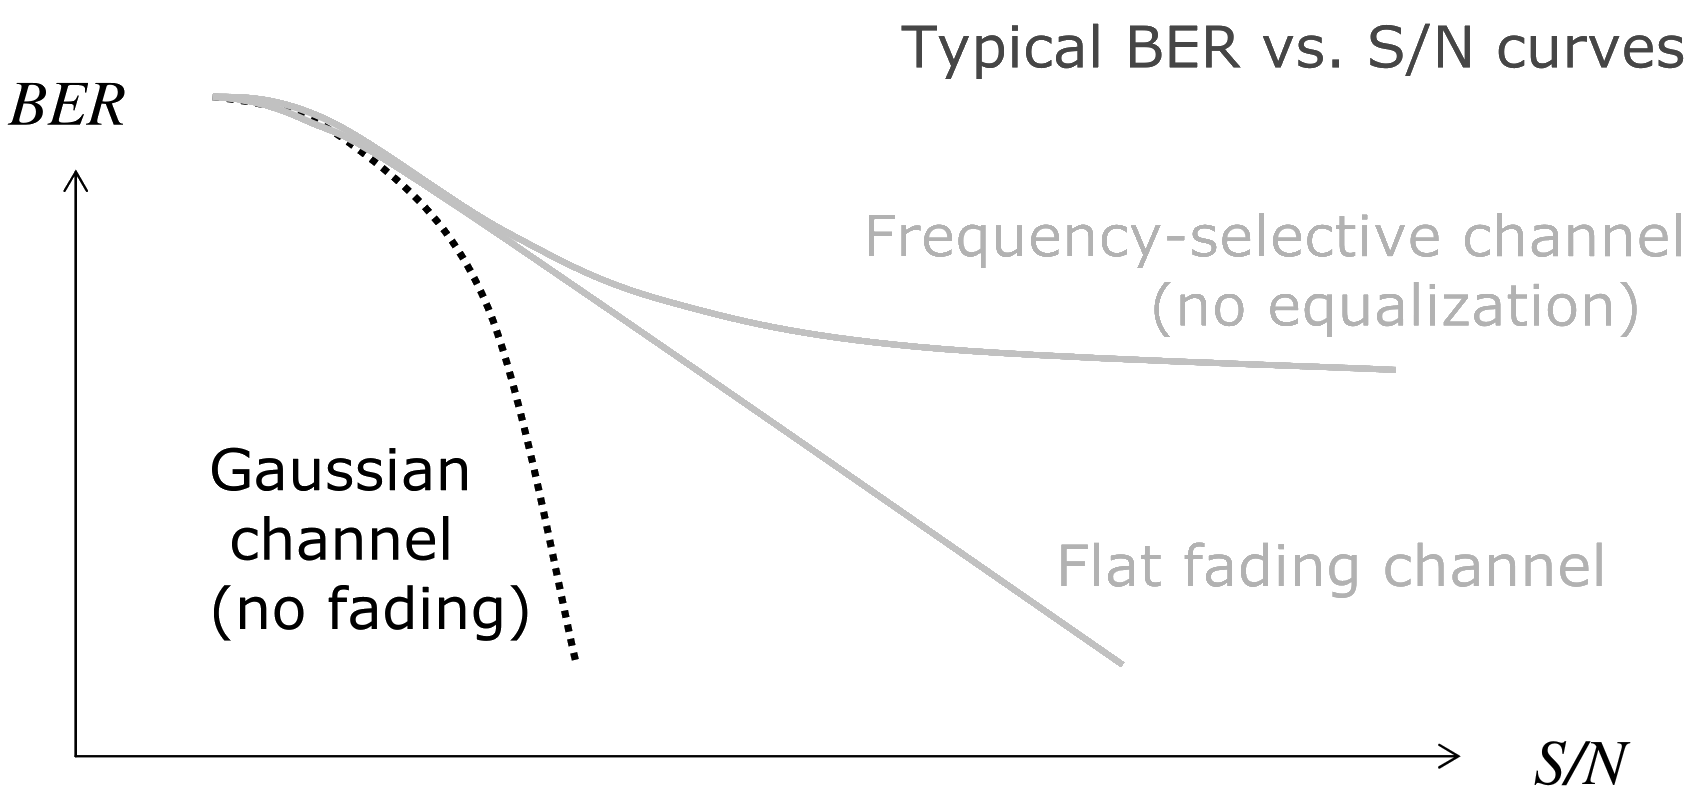
\includegraphics[width=0.675\textwidth]{imgs/bers.png}
\end{figure}


Il fading rappresenta il principale problema nelle comunicazioni radio, sebbene modulazioni come OFDM siano in grado di ridurre l'effetto del multipath fading, tuttavia lo \textbf{slow flat Rayleigh fading} non può essere contrastato nello stesso modo.

\begin{itemize}
    \item \textbf{Slow fading}: $T_c > T$ (Doppler spread)
    \item \textbf{Flat fading}: $\sigma_{\tau}<T$  (multipath time delay spread)
    \item \textbf{Rayleigh fading}: l'attenuazione delle repliche ha una distribuzione di Rayleigh.
\end{itemize}

\begin{figure}[ht]
    \centering
    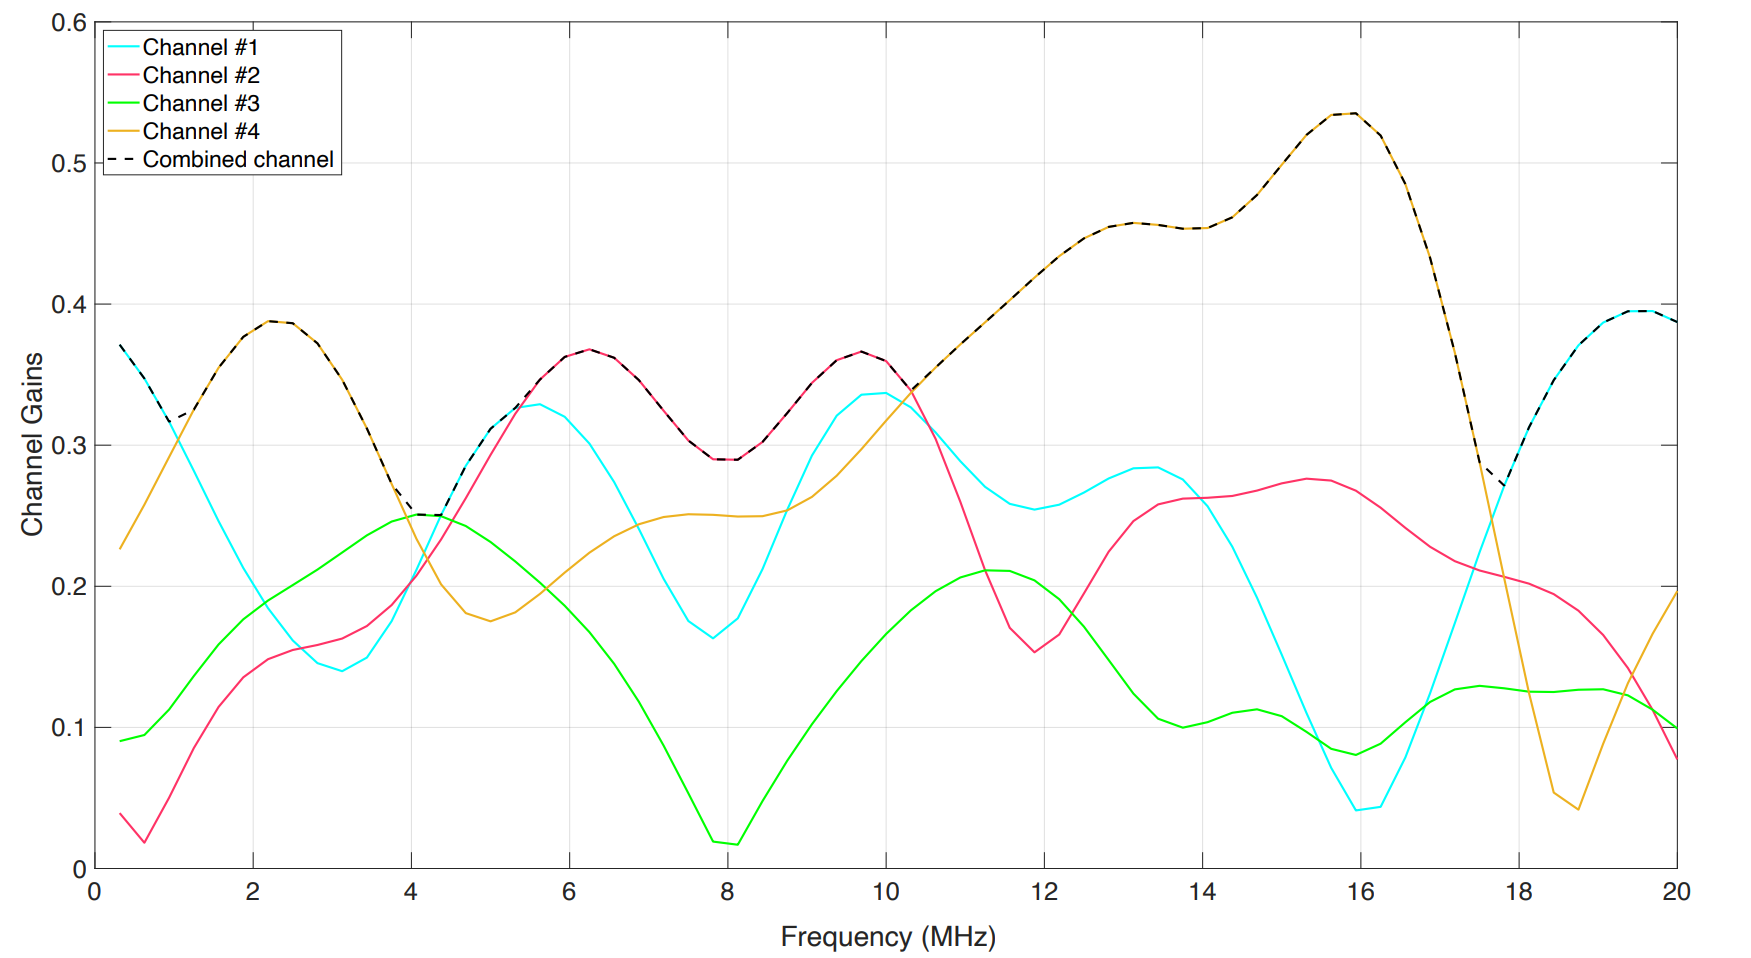
\includegraphics[width=0.675\textwidth]{imgs/diversity_graph.jpg}
\end{figure}


I metodi principali per ridurre gli effetti di un fading di tali tipologie sono le diversity techniques, ovvero lo sfruttamente di canali con caratteristiche differenti per trasmettere la stessa informazione, aumentando la probabilità che il ricevitore possa ricostruire correttamente il messaggio.
Le principali tecniche di diversity sono:
\begin{itemize}
    \item \textbf{Time diversity}: relative al coherence time ($T_c$). Sfruttano trasmmissioni in slot temporali separati utilizzado anche \textbf{coding} e \textbf{interleaving}. Slow fading channels potrebbero non garantire una diversity sufficiente. Il canale deve variare sufficientemente in maniera veloce.
    \item \textbf{Frequency diversity}: relative alla coherence bandwidth ($B_c$). Sfruttano tramissioni su bande differenti. I flat fading channels potrebbero non garantire una diversity sufficiente.
    \item \textbf{Spatial diversity}: relative alla coherence distance. Sfruttano path di propagazione differenti, ad esempio antenne differenti.
\end{itemize}

\subsection*{Time diversity: interleaving and coding}
Il channel coding consiste nell'introdurre dei bit ridondanti insieme a quelli trasmessi per rilevare eventuali errori al ricevitore e migliorare la bit error probability.
La ridondanza è misurata come:
\[
    R = \frac{k}{n} < 1, \quad \begin{cases}
        k \text{ bit contenenti informazione} \\
        n \text{ bit in uscita dall'encoder, contenenti informazione più ridondanza} \\
        n - k \text{ bit di ridondanza}
    \end{cases}
\]

Le operazioni effettuate sfruttano le proprietà matematiche del Galois Field GF(2), su cui sono definite somma (xor) e moltiplicazione (and) per due elementi $\{0, 1\}$.

\begin{figure}[ht]
    \centering
    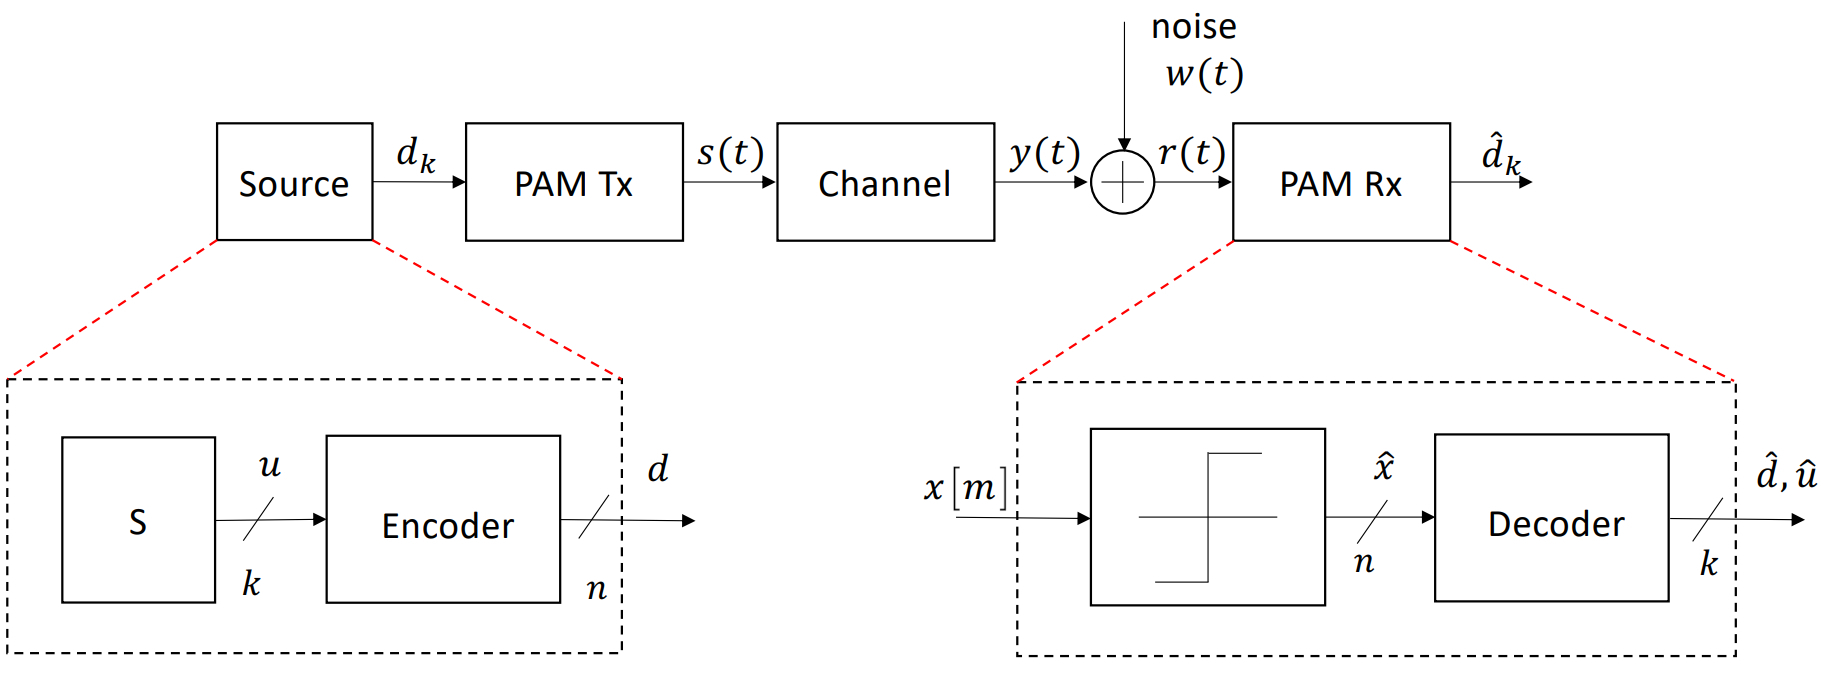
\includegraphics[width=0.675\textwidth]{imgs/encoder_decoder.jpg}
\end{figure}

Sorgente e destinazione introducono \textbf{encoder} e \textbf{decoder} per la gestione dei bit di ridondanza, si può utilizzare lo schema:


\begin{center}
\begin{tikzpicture} [align=center]
    % Draw the block
    
    \node[draw, rectangle, minimum width=2.5cm, minimum height=1.5cm] (block) {Block \\ coder};
    
    % Draw the input arrow
    \draw[-] (block.west) -- ++(-4,0) node[midway, above] {$k$ information digits};
    
    % Draw the output arrow
    \draw[->] (block.east) -- ++(3,0) node[midway, above] {$n$ encoded digits};
\end{tikzpicture}
\end{center}


\begin{center}
    \begin{tikzpicture}[align=center]
    % Draw the main rectangle
    \draw[thick] (0,0) rectangle (5,1);
    
    % Draw the dividing line
    \draw[thick] (3,0) -- (3,1);
    
    % Labels inside the rectangles
    \node at (1.5,0.5) {Information\\digits};
    \node at (4,0.5) {Parity\\digits};
    
    % Arrows and labels
    \draw[<->] (0,1.25) -- (3,1.25) node[midway, above] {$k$};
    \draw[<->] (3,1.25) -- (5,1.25) node[midway, above] {$n-k$};
    \draw[<->] (0,-0.25) -- (5,-0.25) node[midway, below] {$n$ digit codeword};
\end{tikzpicture}

\end{center}

In questo schema l'intero sistema è visto come una componente che aggiunge un errore al messaggio trasmesso.

\paragraph*{Block code}
Si tratta della tipologia più semplice di coding in cui la coded word tramessa è composta da $n-k$ bit di parità.
L'operazione è rappresentabile come operazione di moltiplicazione fra un vettore (word da trasmettere) e una matrice (\textbf{generator matrix}, definisce il tipo di operazione).

\[
    \mathbf{d} = \mathbf{uG}, \quad \begin{cases}
        \mathbf{d} \text{ coded word} \quad d \in GF(2)^{1 \times n} \\
        \mathbf{u} \text{ word da trasmettere} \quad u \in GF(2)^{1 \times k} \\
        \mathbf{G} \text{ generator matrix} \quad G \in GF(2)^{k \times n}
    \end{cases}
\]

In generale le prime $k$ colonne della matrice $G$ equiavalgono a $I_k$ (matrice identità $k \times k$) e le restanti $n-k$ colonne sono i bit di ridondanza.
In totale si possono ottenere $2^k$ codeword differenti (uscita dell'encoder).
Si parla di \textit{coding sistematico} quando i bit di informazione sono semplicemente copiati.

\paragraph*{Error detection}

\begin{center}   
    \begin{tikzpicture}
        % Nodes for the transmitter side
        \node[draw, rectangle, minimum width=1.5cm, minimum height=0.65cm] (T1) at (0,4) {Data 1};
        \node[draw, rectangle, minimum width=1.5cm, minimum height=0.65cm] (T2) at (3,4) {Data 2};
        \node[draw, rectangle, minimum width=1.5cm, minimum height=0.65cm] (T3) at (6,4) {Data 2};
        % create a node containing a red cross
        %\node[draw, cross out, red, thick, minimum size=1cm] (cross) at (4,3) {};
        % create a rotate of 45 degrees
        \node[draw, cross out, red, thick, minimum size=0.5cm, rotate=45] (cross) at (4,3) {};
        % Nodes for the receiver side
        \node[draw, rectangle, minimum width=1.5cm, minimum height=0.65cm] (R1) at (2,2) {Data 1};
        \node[draw, rectangle, minimum width=1.5cm, minimum height=0.65cm] (R2) at (5,2) {Data 2};
        \node[draw, rectangle, minimum width=1.5cm, minimum height=0.65cm] (R3) at (8,2) {Data 2};

        % Arrows for data transmission
        \draw[->, thick] (T1) -- (R1);
        \draw[->, thick] (R1) -- (T2) node[midway, above, sloped] {ACK};
        \draw[->, thick] (T2) -- (R2);
        \draw[->, thick] (R2) -- (T3) node[midway, above, sloped, red] {NACK};
        \draw[->, thick] (T3) -- (R3);

        % Arrow for time
        \draw[<->, dashed] (4.75,1.25) -- (7.75,1.25) node[midway, below] {$T_{ARQ} > T_c$};

        % Vertical lines for transmission boundaries
        \draw[dashed] (4.675,0.5) -- (4.675,3.5);
        \draw[dashed] (7.675,0.5) -- (7.675,3.5);
        
        % Labels for transmissions
        \node at (4.675,0) {1\textsuperscript{st} transmission};
        \node at (7.675,0) {2\textsuperscript{nd} transmission};
        
        % Labels for Transmitter and Receiver
        \node[] at (-2,4) {Transmitter};
        \node[] at (-2,2) {Receiver};
    \end{tikzpicture}
\end{center}



Le tecniche di error detection consistono nel confrontare i bit di ridondanza ricevuti con i bit di ridondanza calcolati utilizzando le word ricevute. 
Se il confronto ha successo si assume che la trasmissione non abbia introdotto errori, altrimenti si rileva un errore nella trasmissione.
In casi di errore il ricevitore può richiedere una nuova trasmissione, adottando lo schema \textbf{ARQ} (Automatic Repeat reQuest).
In tale schema ad ogni ricezione si risponde con un ACK o un NACK, in base al risultato del confronto.
In caso di NACK si procede con una nuova trasmissione. 
Si tratta di una tecnica di time diversity, in quanto la ritrasmissione avviene dopo $T_{ARQ}$, un intervallo temporale superiore al coherence time del canale ($T_{ARQ} > T_c$).
Alcuni ricevitori sono in grado di combinare i due messaggi ricevuti, incrementando la probabilità di ricostruire l'informazione trasmessa.
Una semplice tecnica di error detection è il \textbf{parity check code}, in cui si aggiunge un bit di parità alla fine della word di 7 bit da trasmettere. Se il numero di bit a 1 è pari, il bit di parità è 0, altrimenti è 1.

\[
    \begin{cases}
        k = 7 \\
        n = 8 
    \end{cases}
    \Rightarrow R = \frac{7}{8},
    \quad \mathbf{G} = \left[I_7, 1_7\right] = 
    \begin{bmatrix}
        1 & 0 & 0 & 0 & 0 & 0 & 0 & 1 \\
        0 & 1 & 0 & 0 & 0 & 0 & 0 & 1 \\
        0 & 0 & 1 & 0 & 0 & 0 & 0 & 1 \\
        0 & 0 & 0 & 1 & 0 & 0 & 0 & 1 \\
        0 & 0 & 0 & 0 & 1 & 0 & 0 & 1 \\
        0 & 0 & 0 & 0 & 0 & 1 & 0 & 1 \\
        0 & 0 & 0 & 0 & 0 & 0 & 1 & 1 \\
    \end{bmatrix}
    \Rightarrow u_7 = \sum_{i=0}^{6} u_i
\]
Il parity bit è calcolato sommando tutti i bit delle word usando l'algebra in GF(2).
Sebbene sia molto semplice questa tecnica, non può essere sempre efficace in quanto può riconoscere unicamente un numero di errori dispari, mentre in caso di numero di errori pari si avrà un bilanciamente degli 1 ed il confronto avrà successo.

\paragraph*{Error correction}
Le tecniche di error correction sono utilizzate per rilevare e correggere errori di trasmissione, senza necessità di richiedere una nuova trasmissione.
Dato un canale si definisce \textbf{capacità} il massimo rate a cui è possibile trasmettere:
\[
    C = B \log_2(1 + \text{SNR}) \quad \text{bit/s}
\]

Ogni trasmissione con rate $R < C$ ed $\epsilon$ arbitratio è possibile determinare un error correction code per cui $P_e < \epsilon$.
Una semplice tecnica di error correction è il \textbf{repetition code}, in cui la word è ripetuta 3 volte. 
Per stabilire quale sia il bit corretto in casi di incongruenza si adotta una strategia maggioritaria.


\[
    \begin{cases}
        k = 1 \\
        n = 3 
    \end{cases}
    \Rightarrow R = \frac{1}{3},
    \quad \mathbf{G} =
    \begin{bmatrix}
        1 & 1 & 1
    \end{bmatrix}
    \quad 
    \begin{cases}
        u = \begin{bmatrix}0\end{bmatrix} \Rightarrow d = \begin{bmatrix}0 & 0 & 0\end{bmatrix} \\
        \\
        u = \begin{bmatrix}1\end{bmatrix} \Rightarrow d = \begin{bmatrix}1 & 1 & 1\end{bmatrix}
    \end{cases}
\]


Questa tecnica è in grado di correggere un unico errore, tuttavia se utilizzato come error detection può rilevare fino a due errori.
La distanza tra due codeword è calcolata come numero di bit differenti fra le due stringhe, detta anche \textbf{Hamming distance}. Il decoder selezione le word con minima distanza rispetto a quella ricevuta.

\[
%\hat{a}_m = \underset{i=1,\ldots,M}{\mathrm{argmin}}
    \hat{d} = \underset{d}{\mathrm{argmin}} \left\{\text{distance}(d, \hat{x})\right\}
\]

Dove $\hat{d}$ è la word in uscita dal decoder, $d$ è una word possibile e $\hat{x}$ è la word ricevuta
Gli errori possono far scegliere al decoder la word sbagliata, la capacità di error correction di un block code è tanto maggiore quanto maggiore è la Hamming distance tra le codeword generabili. La bontà del block code è misurabile con la minima distanza tra codewords $d_{min}$.
\[
    d_{min} - 1 \quad \text{Numero massimo di errori rilevabili}
\]

\[
    \left\lfloor \frac{d_{min} - 1}{2} \right\rfloor \quad \text{Numero massimo di errori correggibili}
\]
Maggiore è la distanza di Hamming, maggiore è la ridondanza da aggiungere.
Fissata $R=\frac{k}{n}$, $d_{min}$ sarà più grande al crescere di $k$ e $n$, tuttavia si complica anche il sistema.
\section*{Convolutional code}

I codici convoluzionali, al contrario dei block code, non sono sistematici, si trasmettono infatti solo i bit di parità.
L'encoder utilizza una sliding window per generare $n>1$ bit di parità, combinando vari sottoinsiemi di bit nel campo GF(2), realizzando una sorta di convoluzione.
L'encoder si comporta come $n$ filtri lineari in parallelo, i parametri che lo costituiscono sono:
\begin{itemize}
    \item $n$: bit generati
    \item $k$: bit di informazione (si considererà sempre $k=1$)
    \item $L$: lunghezza del vincolo, ovvero il numero di parole di input di $k$ bit che concorrono alla generazione degli $n$ bit di output. Nel caso di $k=1$ sarà la lunghezza dei bit che concorrono alla generazione del codice.
\end{itemize}

La dimensione della finestra corrisponde a $L-k$, quindi si considererà $L-1$. Il codice generato, oltre alla word, è anche funzione dei bit di input precedenti. Ogni bit generato è ottenuto dalla convoluzione in GF(2) con una risposta impulsiva rappresentata da un diverso generatore $g$, di dimensione $kL$.
Possiamo considerare come analogia in $\mathbb{R}$ la convoluzione tra un segnale e la risposta impulsiva di un filtro la cui espressione è:
\[
    y\left[k\right] = \sum_{m=0}^{M-1} g\left[m\right] \cdot x\left[k-m\right]
\]
Per i codici convoluzionali, che operano in GF(2), similmente scriveremo:
\[
    d_j^{\left(i\right)} = \sum_{\ell=0}^{L-1} g_j\left(\ell\right) \cdot u^{\left( i - \ell \right)}
\]

I bit in uscita sono quindi un flusso continuo e non organizzati in blocchi.

Trattandosi di sistemi con memoria, l'encoder può essere rappresentato come una macchina a stati finiti.
L'output dell'encoder dipende dal bit in input e dalla stato corrente.
L'evoluzione temporale dell'encoder può essere catturata dal \textbf{trellis diagram}, in cui si ha l'evoluzione degli stati in funzione del tempo.
Ogni sequenza, con la corrispondente encoded word, può essere rappresentata come un cammino nel trellis diagram.
Una trasmissione di $N$ codewords implica la trasmissione di $n \cdot N$ bits, ottenuti dalla codifica di $k \cdot N$ input word.
Poiché ogni codeword è funzione anche di $L-1$ input word precedenti, la sequenza può essere codificata considerandola solo nella sua interezza. 
Il decoder dovrà scegliere la sequenza più "vicina" rispetto a quella ricevuta tra tutte le possibili sequenza, ovvero $2^{k \cdot N}$
\[
    \hat{d} = \underset{d}{\text{argmin}} \left\{\text{distance}(d, \hat{x})\right\}
\]
Dove $d$ è una possibile sequenza, $\hat{x}$ è la sequenza ricevuta e $\hat{d}$ è la sequenza in uscita dal decoder.
L'utilizzo nella pratica di codici convoluzionali è stata resa possibile solo dall'introduzione dell'algoritmo di Viterbi, in grado di applicare una decodifica con complessità lineare e non più esponenziale.

\paragraph*{Codice convoluzionale (2, 1, 3)}

In un codice convoluzionale (2, 1, 3), ovvero con parametri $n=2$, $k=1$ e $L=3$, supponiamo di avere come generatori (che si possono dimostrare essere ottimi):
\[
    g_1 = \begin{bmatrix}1 & 1 & 1\end{bmatrix}, \quad g_2 = \begin{bmatrix}1 & 0 & 1\end{bmatrix}
\]

Come si può notare, la dimensione dei generatori è $kL = 1 \cdot 3 = 3$, il code rate è $R = \frac{k}{n} = \frac{1}{2}$, mentre la memoria è $L - 1 = 3 - 1 = 2$.
\begin{center}
    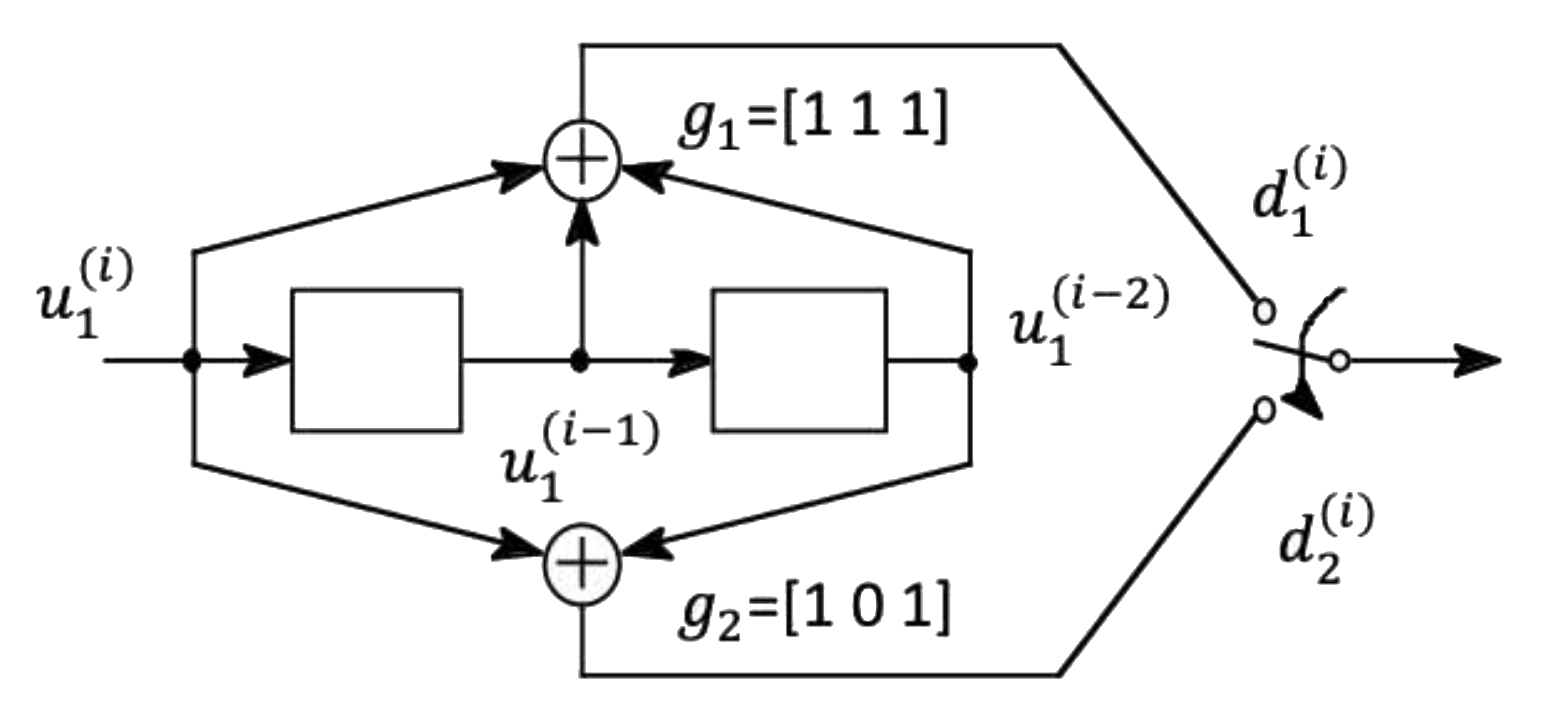
\includegraphics[width=0.5\textwidth]{imgs/213code.png}
\end{center}

Nella figura è possibile notare come siano presenti 2 elementi di memoria (i due rettangoli bianchi), ovvero i $k(L-1)$ elementi di memoria che sono sufficienti a rappresentare lo stato dell'encoder.
Le codeword di output, applicando quindi la convoluzione tra i bit di input e i generatori, sono:
\[
    d_1^{\left(i\right)} = \sum_{\ell=0}^{2} g_1\left(\ell\right) \cdot u^{\left( i - \ell \right)} = u^{\left(i\right)} + u^{\left(i-1\right)} + u^{\left(i-2\right)}
\]

\[
    d_2^{\left(i\right)} = \sum_{\ell=0}^{2} g_2\left(\ell\right) \cdot u^{\left( i - \ell \right)} = u^{\left(i\right)} + u^{\left(i-2\right)}
\]

Possiamo definire una macchina a stati fatta nella seguente maniera:

\begin{center}
\begin{tikzpicture}[shorten >=1pt, node distance=3cm, on grid, auto]
   \node[state] (q_11)   {11};
   \node[state] (q_10) [below left=of q_11] {10};
   \node[state] (q_01) [below right=of q_11] {01};
   \node[state] (q_00) [below right=of q_10] {00};

    \path[->]
    (q_11) edge [loop above] node {1/10} ()
          edge [bend left=15] node {0/01} (q_01)
    (q_10) edge [bend right=15] node [above] {1/00} (q_01)
          edge [bend left=15] node [right] {1/01} (q_11)
    (q_01) edge [bend left=15] node [right] {0/11} (q_00)
          edge [bend right=15] node [above] {0/10} (q_10)
    (q_00) edge [loop below] node {0/00} ()
          edge [bend left=15] node {1/11} (q_10);
\end{tikzpicture}
\end{center}


Dove i nodi rappresentano lo stato dell'encoder, ovvero i bit di memoria, mentre gli archi rappresentano separati dallo slash rispettivamente il bit di input e l'output.
La macchina a stati è ricavabile col seguente codice:

\begin{minted}{python3}
G1 = [True, True, True]
G2 = [True, False, True]

G = [G1, G2]

def next_state(input_bit: bool, state: Tuple[bool, bool]):
    d = [(g[0] & input_bit) ^ (g[1] & state[0]) ^ (g[2] & state[1]) for g in G]
    return (input_bit, state[0]), (d[0], d[1])
\end{minted}

La funzione \textit{next\_state} prende in input il bit da codificare e lo stato corrente dell'encoder, restituendo lo stato successivo, ottenuto con una sorta di shift, e i bit di output.

\paragraph*{Algoritmo di Viterbi}
L'obiettivo è trovare la sequenza con distanza minima rispetto a quella ricevuta:

\[
    \hat{d} = \underset{d}{\text{argmin}} \left( d_H \left(\tilde{d}, \hat{x}\right) \right)
\]
Le possibili sequenza $\tilde{d}$ sono viste come sequene di $N$ blocchi, ciascuna composta da 
$n$ bit, ovver i bit prodotti a partire dai $k$ bit di informaione in ingresso all'encoder.


\[
    d_H\left(\tilde{d}, \hat{x}\right) = \sum_{j=1}^{N} d_H\left(\tilde{d}_j, \hat{x}_j\right)
\]

Dove $d_H$ è la distanza di Hamming tra due sequenze di bit, $\tilde{d}_j$ è la $j$-esima codeword possibile e $\hat{x}_j$ è la $j$-esima codeword ricevuta.
Ogni sequenza $\tilde{d}$ corrisponde ad una seuqenza di stati $\tilde{S}_0, \ldots, \tilde{S}_N$ nel diagramma a trabocco, ovvero a un determinato path. La $j$-esima uscita dell'encoder, $\tilde{d}_j$, dipende dalla transizione tra gli stati $\tilde{S}_{j-1}$ e $\tilde{S}_j$.
.
.
.
.

% insert python code hello world hre
La distanza di Hamming può essere calcolata in Python come:
\begin{minted}{python3}
def hamming_distance(a: int, b: int) -> int:
    return bin(a ^ b).count('1')
\end{minted}


Dal Trellis diagram possiamo dedurre la funzione di transizione come:
\begin{minted}{python3}

def state_machine(state: int, input_bit: bool) -> Tuple[int, int]:
    match state:
        case 0b01:
            return (0b11, 0b00) if not input_bit else (0b00, 0b10)
        case 0b10:
            return (0b10, 0b01) if not input_bit else (0b01, 0b11)
        case 0b11:
            return (0b01, 0b01) if not input_bit else (0b10, 0b11)
        case 0b00:
            return (0b00, 0b00) if not input_bit else (0b11, 0b10)
        case _:
            raise ValueError("Invalid state")

\end{minted}
Per quanto riguarda invece l'algoritmo di Viterbi, esso può essere definito per sommi capi come:

\begin{minted}{python3}
def viterbi_algorithm(sequence: List[bool]) -> List[bool]:
    # [a_0, a_1, a_2, a_3, ...] -> [a_0 * 2 + a_1, a_2 * 2 + a_3, ...]
    outputs: List[int] = bit_pairs_to_integers(sequence)
    matrix: List[List[Optional[ViterbiCell]]] = populate_matrix(outputs)
    final_state = get_last_state(matrix)
    return get_decoded_sequence(matrix, final_state)
\end{minted}

La funzione \textit{populate\_matrix} riempie una matrice con celle di Viterbi aggiornando distanze globali e stati successivi per ogni colonna di output. Con il termine output indicheremo l'output dell'encoder che abbiamo ricevuto e quindi che dovremo, sfruttano anche lo stato del sistema, trasformare nel bit di input originario, ovvero l'$i$-esimo bit della sequenza che effettivamente si voleva trasmettere. Il numero di riga corrisponde al possibile stato.
\begin{minted}{python3}
def populate_matrix(outputs: List[int]) -> List[List[Optional[ViterbiCell]]]:
    matrix: List[List[Optional[ViterbiCell]]] = empty_matrix(rows=4, cols=len(outputs) + 1)
    matrix[0][0] = ViterbiCell(prev_state=0, global_distance=0, input_bit=False)

    for col in range(len(outputs)):
        target_output = outputs[col]
        for row in range(4):
            current_cell = matrix[row][col]
            if current_cell is None:
                continue
            for input_bit in [False, True]:
                output, next_state = state_machine(row, input_bit)
                new_distance = current_cell.global_distance + hamming_distance(output, target_output)
                next_cell = matrix[next_state][col + 1]
                if next_cell is None or next_cell.global_distance > new_distance:
                    matrix[next_state][col + 1] = ViterbiCell(
                        row, new_distance, input_bit
                    )
    return matrix
\end{minted}

La funzione \textit{get\_last\_state} trova lo stato finale con la distanza globale minima nell'ultima colonna della matrice.
\begin{minted}{python3}
def get_last_state(matrix: List[List[Optional[ViterbiCell]]]) -> int:
    min_distance = float('inf')
    final_state = None
    last_column = [matrix[i][-1] for i in range(4)]
    for row, cell in enumerate(last_column):
        if cell and cell.global_distance < min_distance:
            min_distance = cell.global_distance
            final_state = row
    return final_state
\end{minted}
La funzione \textit{get\_decoded\_sequence} ricostruisce la sequenza decodificata risalendo dalla matrice a partire dallo stato finale.
\begin{minted}{python3}
def get_decoded_sequence(matrix: List[List[Optional[ViterbiCell]]], final_state: int) -> List[bool]:
    sequence_length = len(matrix[0]) - 1
    decoded_sequence: List[bool] = [False] * sequence_length
    
    current_state = final_state
    for i in range(sequence_length - 1, -1, -1):
        cell = matrix[current_state][i + 1]
        decoded_sequence[i] = cell.input_bit
        current_state = cell.prev_state

    return decoded_sequence
\end{minted}


Come esempio consideriamo di voler trasmettere la sequenza di bit $010000$, l'encoder emetterà quindi la sequenza $00 \ 11 \ 10 \ 11 \ 00 \ 00$. Supponendo che il decoder riceva la sequenza $00 \ 10 \ 10 \ 11 \ 00 \ 00$, l'algoritmo di Viterbi sarà in grado di correggere l'errore e restituire la sequenza corretta $010000$.




\begin{center}
    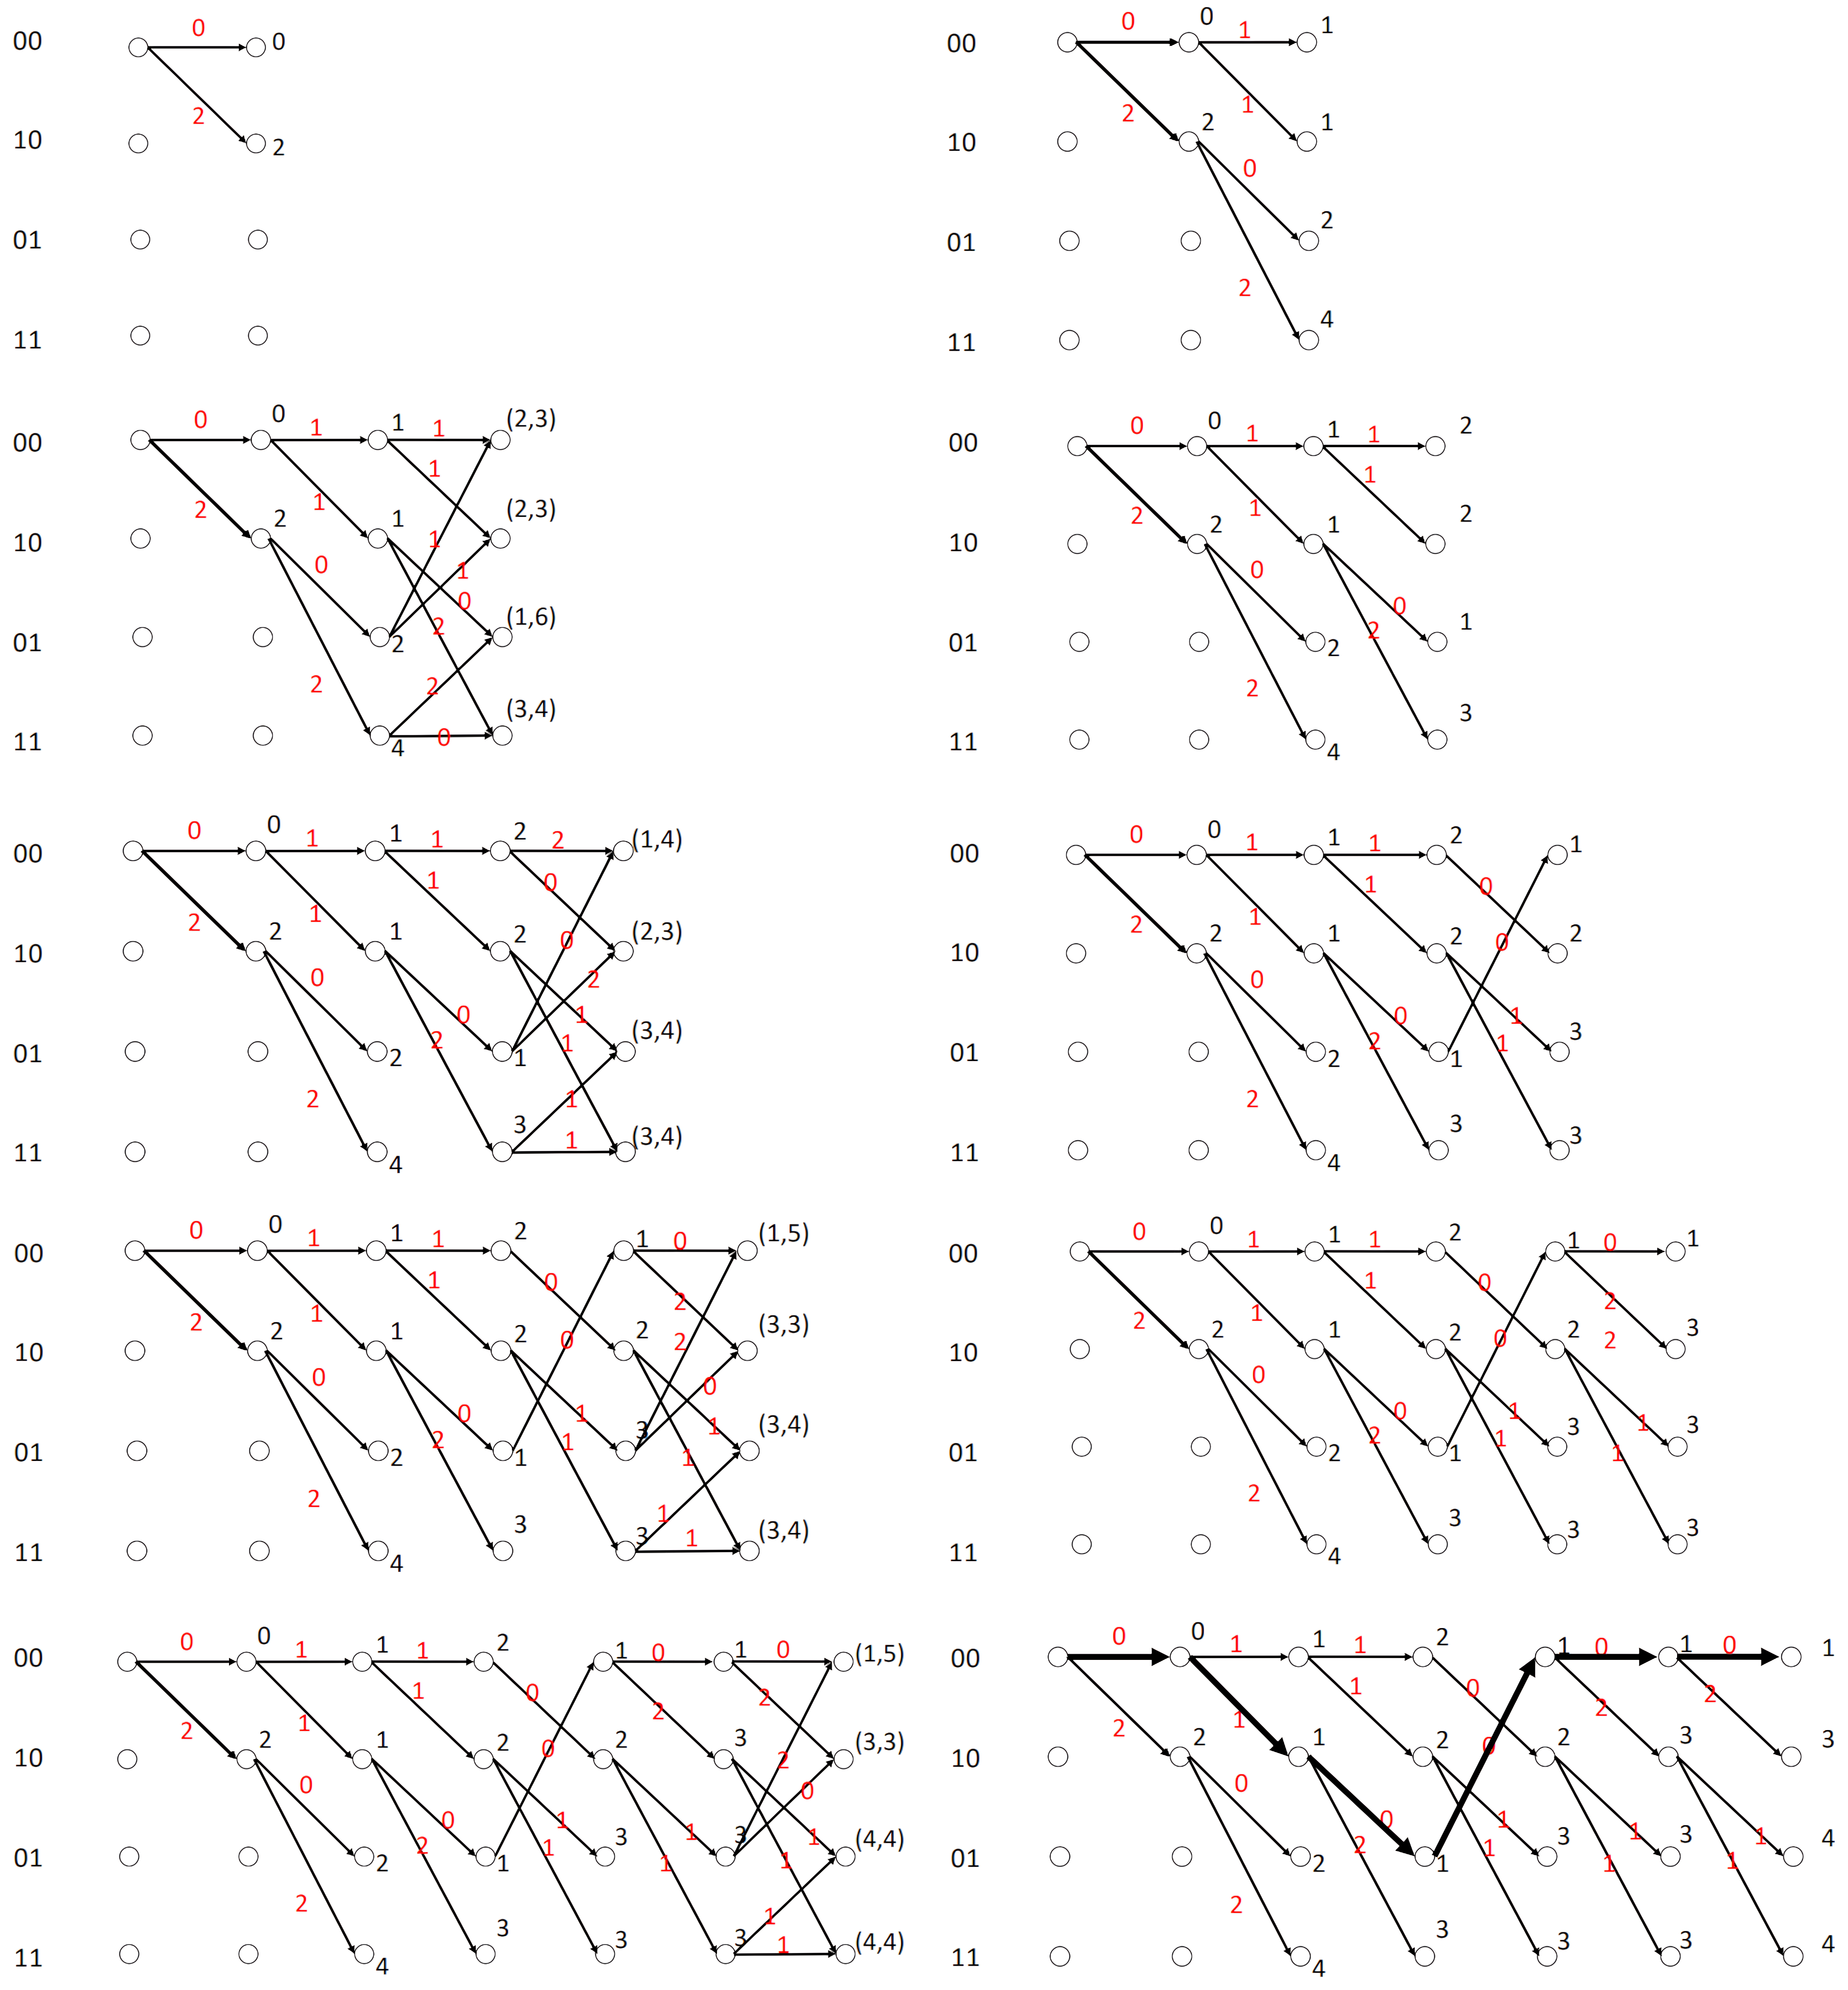
\includegraphics[width=1\textwidth]{imgs/viterbi_example.png}
\end{center}


Ovvero eseguendo l'algoritmo in Python si ottiene la seguente rappresentazione in memoria, stampando i campi \textit{prev\_state}, \textit{global\_distance} e \textit{input\_bit} per ogni cella della matrice:


\begin{table}[h!]

\resizebox{\textwidth}{!}{
    \centering
    \begin{tabular}{|c|c|c|c|c|c|c|c|}
    \hline
    State & Column 1 & Column 2 & Column 3 & Column 4 & Column 5 & Column 6 & Column 7 \\
    \hline
    Row 0b00 & 0b00, 0, 0 & \textbf{0b00, 0, \textcolor{red}{0}} & 0b00, 1, 0 & 0b00, 2, 0 & \textbf{0b01, 1, \textcolor{red}{0}} & \textbf{0b00, 1, \textcolor{red}{0}} & \textbf{0b00, 1, \textcolor{red}{0}} \\
    \hline
    Row 0b10 & None & 0b00, 2, 1 & \textbf{0b00, 1, \textcolor{red}{1}} & 0b00, 2, 1 & 0b00, 2, 1 & 0b00, 3, 1 & 0b00, 3, 1 \\
    \hline
    Row 0b01 & None & None & 0b10, 2, 0 & \textbf{0b10, 1, \textcolor{red}{0}} & 0b10, 3, 0 & 0b10, 3, 0 & 0b10, 4, 0 \\
    \hline
    Row 0b11 & None & None & 0b10, 4, 1 & 0b10, 3, 1 & 0b10, 3, 1 & 0b10, 3, 1 & 0b10, 4, 1 \\
    \hline
    \end{tabular} 
        
    }
    \end{table}

\section*{Interleaving}



\begin{center}
    \resizebox{\textwidth}{!}{
    \begin{tikzpicture}[node distance=1.5cm, auto, >=Stealth, minimum height=1cm, minimum width=1.5cm]
        % Nodes
        \node[draw, rectangle] (S) {S};
        \node[draw, rectangle, right=of S] (Encoder) {Encoder};
        \node[draw, rectangle, right=of Encoder] (Interleaver) {Interleaver};
        \node[draw, rectangle, right=of Interleaver] (Channel) {Channel};
        \node[draw, rectangle, right=of Channel] (Deinterleaver) {Deinterleaver};
        \node[draw, rectangle, right=of Deinterleaver] (Decoder) {Decoder};
        \node[right=of Decoder, inner sep=0pt, minimum size=0pt] (Uhat) {};

        % Connections
        \draw[->] (S) -- node {$u$} (Encoder);
        \draw[->] (Encoder) -- (Interleaver);
        \draw[->] (Interleaver) -- node {$d$} (Channel);
        \draw[->] (Channel) -- node {$x$} (Deinterleaver);
        \draw[->] (Deinterleaver) -- (Decoder);
        \draw[->] (Decoder) -- node {$\hat{u}$} (Uhat);


        % Dashed boxes
        \draw[dashed] ($(S.north west)+(-0.5,0.5)$) rectangle ($(Interleaver.south east)+(0.5,-0.5)$);
        \draw[dashed] ($(Deinterleaver.north west)+(-0.5,0.5)$) rectangle ($(Decoder.south east)+(0.5,-0.5)$);
    \end{tikzpicture}
}
\end{center}
\begin{center}
    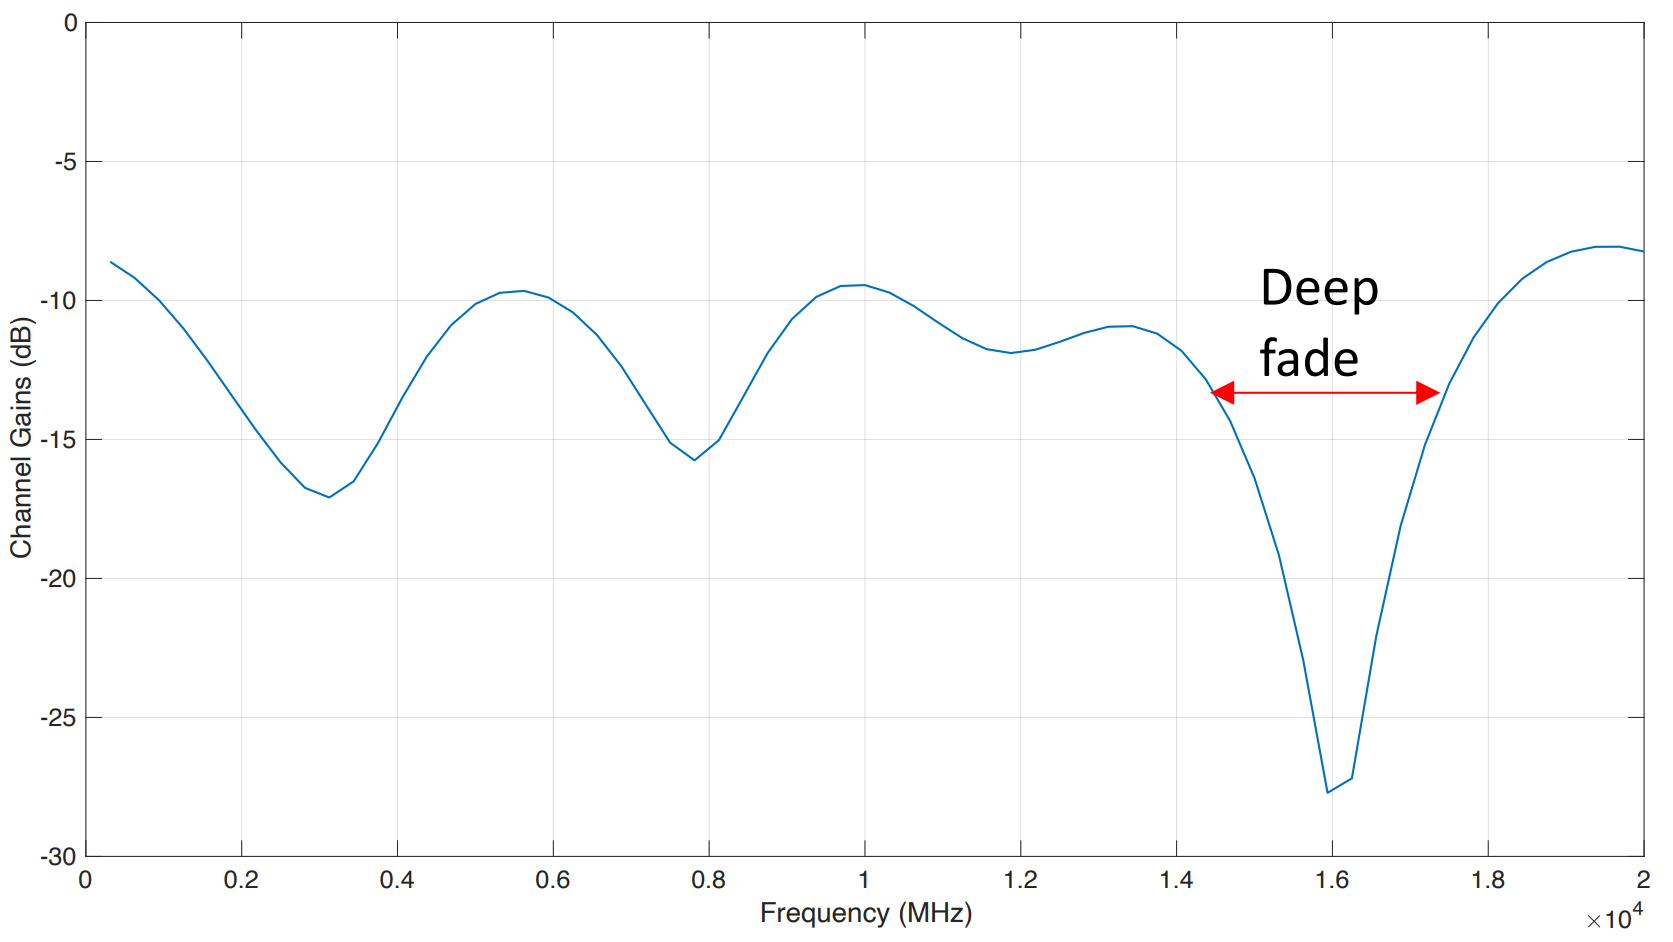
\includegraphics[width=0.5\textwidth]{imgs/deep_fade.png}
\end{center}

I codici convoluzionali risultano adatti per canali memoryless con errori randomici, uniformamente distribuiti ed incorrelati. 
Tuttavia un canale fading è tipicamente suggetto a \textbf{bursty errors}, ovvero genera un gruppo di errori consecutivi nel tempo e/o in frequenza. 
Quando il canale è in \textbf{deep fade} ci sono delle dipendenze statistiche tra errori consecutivi.
L'idea dell'interleaving consiste nel far sembrare il canale memoryless dal punto di vista del decoder, de-correlando gli errori provocati dal canale, semplicemente rimescolando i bit prodotti dell'encoder prima di effettuare la trasmissione.
Lato ricevitore prima del decoder si effettuare un'operazione di de-interleaving per ripristinare l'ordine originale.
Il costo delle operazioni di (de-)interleaving è pagato in termini di latenza in quanto sia lato ricevitore che lato trasmettitore è necessario avere un intero blocco di dati prima di poter effettuare le operazioni. 
Esiste un trade-off tra latenza e decorrelazione ottenibile, basata sulla profondità $k$ dell'interleaver, ovvero la dimensione del blocco sul quale si effettua l'operazione di rimescolamento.

Per esempio disponendo una sequenza dentro una matrice, possiamo ottenere un interleaver considerando la trasposta:
\begin{table}[h!]
    \centering
    \begin{tabular}{c}
    
    \begin{tabular}{|c|c|c|c|}
    \hline
    A & B & C & D \\ \hline
    E & F & G & H \\ \hline
    I & J & K & L \\ \hline
    M & N & O & P \\ \hline
    \end{tabular}
    
    \quad $\rightarrow$ \quad
    
    \begin{tabular}{|c|c|c|c|}
    \hline
    A & E & I & M \\ \hline
    B & F & J & N \\ \hline
    C & G & K & O \\ \hline
    D & H & L & P \\ \hline
    \end{tabular}
    
    \end{tabular}
\end{table}
   

\begin{center}
    \resizebox{\textwidth}{!}{
    \begin{tikzpicture}
        \node (input) at (0,0) {$\{A,B,C,D,E,F,G,H,I,J,K,L,M,N,O,P\}$};
        \node[draw, minimum height=2cm, minimum width=3cm, align=center] (interleaver) at (6,0) {Interleaver};
        \node (output) at (12,0) {$\{A,E,I,M,B,F,J,N,C,G,K,O,D,H,L,P\}$};

        \draw[->] (input) -- (interleaver);
        \draw[->] (interleaver) -- (output);
    \end{tikzpicture}
    }
\end{center}



\paragraph*{Turbo code e LDPC (Low Density Parity Check)}
Nella formula della capacità del canale di Shannon\footnote{$C=B\log_2(1+\text{SNR}) \si{b/s}$} il rate $R = \frac{k}{n}$ prevede sia $k$ che $n$ tendenti all'infinito, tuttavia la lunghezza del codice nei sistemi reali è finito, quindi ciò che si ottiene è una performance lontana da quella teorica.
Negli anni sono stati introdotti nuovi codici, sempre più efficienti, tra cui turbo code e LDPC, i quali si avvicinano al limite teorico imposto dalla formula di Shannon.


Più nel dettaglio abbiamo lato trasmettitore da eseguire i seguenti passi:

\begin{center}
    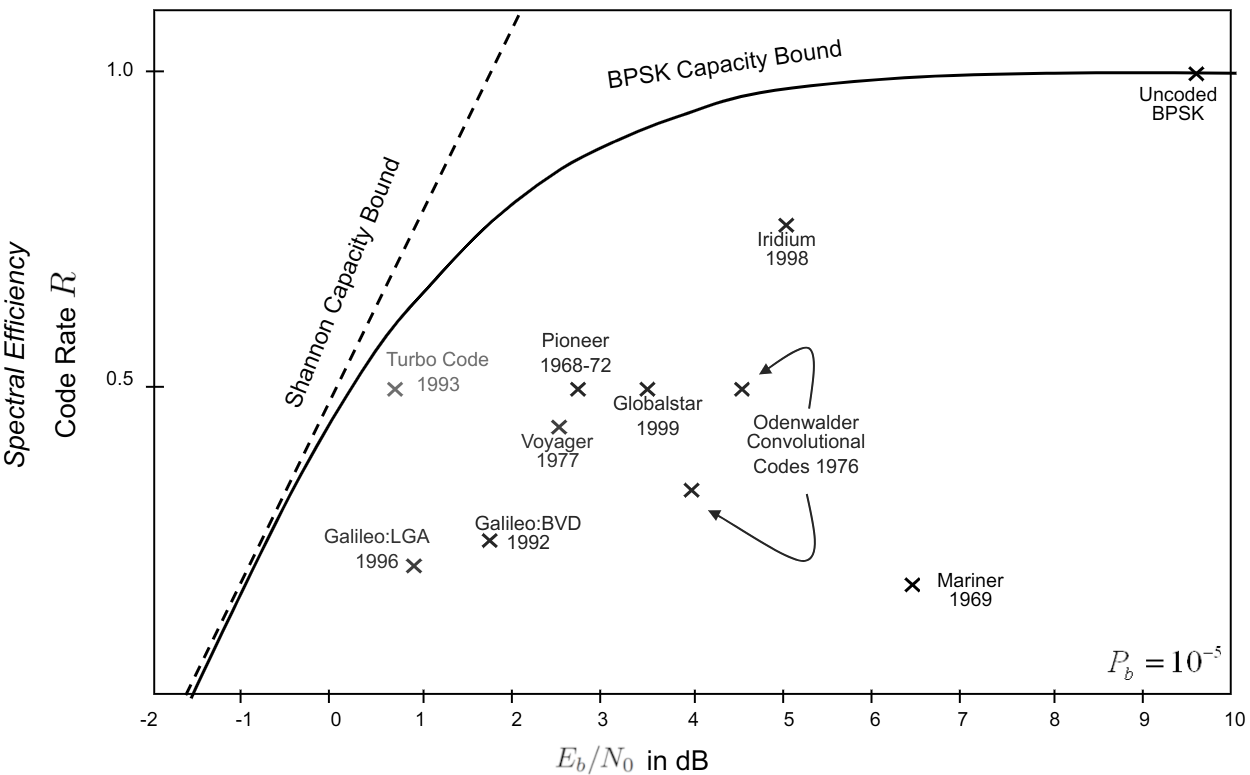
\includegraphics[width=0.5\textwidth]{imgs/codes_and_shannon_bound.png}
\end{center}
\paragraph*{Turbo code (error correction)}

Si tratta di un convolutional code in cui sono utilizzati due encoder in parallelo in grado di generare due sequenze indipendenti, migliorando il processo di decoding grazie alla ridondanza ottenuta e alla diversity, ottenuta dalla presenza di uno stream di dati differente.
Il sistema è composto da tre sequenze di cui due codificate e una inalterata. L'utilizzo dell'interleaver permette di estendere artificialmente la lunghezza della sequenza, avvicinandosi alle ipotesi di Shannon. Inoltre l'interleaver permette di ottenere sequenze indipendenti. 
Il trasmettitore invia quindi tre sequenze, tra cui quella originaria, ottenendo un $R=\frac{1}{3}$. L'idea è che se il canale produce un errore le due sequenze prodotte in maniera differente possono essere unite  per correggere l'errore.
Per quanto riguarda il decoder si utilizzano due decoder in cascata, il primo prevede in ingresso i bit sistematici e la prima sequenza generanza senza interleaving. L'output prodotto invece di essere utilizzato come uscita del sistema è inviato ad un inteleaver, assieme ai bit sistematici. 
Le due sequenze dopo l'interleaving sono mandate in ingresso, assieme alla seconda sequenza di parità, al secondo decoder. L'uscita è infine inviata al deinterleaver. 
Completato il primo ciclo è possibile effettuarne altri, mandando nuovamente in ingresso al primo decoder l'uscita dell'interleaver. 
L'uscita dei decoder rappresenta una stima, sempre più accurata, della sequenza trasmessa. Il processo iterativo va avanti finché vi sono modifiche nei bit decifrati.
In generale se il SNR rispetta le condizioni di Shannon l'impiego di turbo codes permette di effettuare la correzione degli errori ed ottenere dei BER molto bassi, tuttavia il prezzo è ancora pagato in termini di latenza.






\begin{center}

    \begin{figure}[h!]
        \centering
        \begin{tikzpicture}
    
            % Draw blocks
            \node[draw, rectangle] (RSC1) at (3,2) {RSC1};
            % dummy node for alignment
            \node[inner sep=0pt, minimum size=0pt] (dummy) at (3,1) {};
            \node[draw, rectangle] (Interleaver) at (0,0) {Interleaver};
            \node[draw, rectangle] (RSC2) at (3,0) {RSC2};
            
            \draw[->] (0,2) -- (RSC1) node[midway, above] {};
            \draw[->] (RSC1) -- (5,2) node[midway, above] {$d^{(1)} = p_1$};
            \draw[->] (Interleaver) -- (RSC2);
            \draw[->] (RSC2) -- (5,0) node[midway, above]{$d^{(2)} = p_2$}; 
            \draw[->] (-1,1) -- (5,1) node[midway, above, xshift=63, yshift=2] {$d^{(0)} = u$};
            \draw[-] (Interleaver) -- (0, 2) node[midway, left] {}; 
            \node at (-0.2,1.2) {$u$};
            
        \end{tikzpicture}
        \caption{}
       
        \label{fig:turbo_encoder}
    \end{figure}
\end{center}
\begin{enumerate}
    \item I bit di informazione (e.g. $01101$) entrano nel trasmettitore e vengono copiati negli encoder RSC1 RSC2. Prima di entrare in RSC2, i bit di informazione vengono rimescolati dall'interleaver (e.g. $10011$).
    \item Ogni encoder genera una stringa di bit di correzione di errore (bit di parità) eseguendo una serie di calcoli sui bit di dati che riceve (e.g. rispettivamente, $10110$ e $11100$).
    \item I bit di informazione e le due stringhe di bit di parità sono combinati in un unico blocco e inviati sul canale, dove il rumore può causare errori nella trasmissione.
\end{enumerate}

Per quanto rigurda la ricezione, il processo è il seguente:

\begin{center}
    \begin{tikzpicture}[node distance=1.5cm, auto, >=Stealth, minimum height=1cm, minimum width=1.5cm]

        \node[draw, rectangle] (D1) at (3,0) {D1};
        \node[draw, rectangle] (I) at (6,0) {I};
        \node[draw, rectangle] (D2) at (9,0) {D2};
        \node[draw, rectangle] (InvI) at (6,2) {Inv(I)};

        \draw[->] (0,0) -- (2.25, 0) node[midway, above] {$\hat{p}_1$};
        \draw[->] (0,-0.875) -| (D1) node[midway, below] {$\hat{u}$};
        \draw[->] (0,-1.75) -| (I) node[midway, below] {$\hat{p}_2$};
        \draw[->] (3,-0.875) -| (5.675, -0.5) node[midway, below] {};
        \draw[->] (D1) -- (I) node[midway, above] {Le12};
        \draw[->] (I) -- (D2);
        \draw[->] (D2) |- (InvI) node[midway, right] {Le21};
        \draw[->] (InvI) -| (D1);
        % TODO: a cosa serve la seconda freccia?
        %\draw[->] (6.25, -0.5) -- ++(0,-0.875) -| (D2);
    \end{tikzpicture}
\end{center}



\begin{enumerate}
    \item Al segnale (campionato) viene associata una lista di interi (e.g. $[7, -5, 5, 2, -4; \ 6, 5, 7 -2, \textcolor{red}{-2}; \ 3, 8, 1, -5, -3]$, dove $\hat{p}_1$, $\hat{u}$ e $\hat{p}_2$ sono stati separati da un punto e virgola, mentre il rosso è idicata una predizione sbagliata), 
    i cui elementi indicano quanto è probabile che un bit sia 0 o 1. Ad esempio, -7 significa che il bit è quasi certamente un 0; +7 significa che è quasi certamente un 1. Notare che un errore è avvenuto nel quinto bit del blocco: originariamente un 1, ora ha un valore negativo, che suggerisce un 0 logico.
    \item Ogni decoder prende la lista contenente l'informazione con rumore e la rispettiva lista di parità e calcola quanto è sicuro di ciascun bit decodificato. I due decoder scambiano queste informazioni di confidenza ripetutamente e dopo un certo numero di iterazioni, tipicamente da quattro a dieci, iniziano ad essere d'accordo su tutti i bit decodificati. 
    \item I dati decodificati sono la somma della lista contenente l'informazione (con rumore, e.g. $[6, 5, 7 -2, \textcolor{red}{-2}]$) più le due liste finali contenti i valori di confidenza(e.g. $[-5, 3, 7, -6, 5]$ e $[-3, 4, 2, -4, 3]$). L'output ($[-14, 12, 16, -12, 6]$) viene convertito nuovamente in bit binari ($[0, 1, 1, 0, 1]$,  da cui si può notare che il quinto bit ora ha il valore corretto).
\end{enumerate}



\begin{center}
    
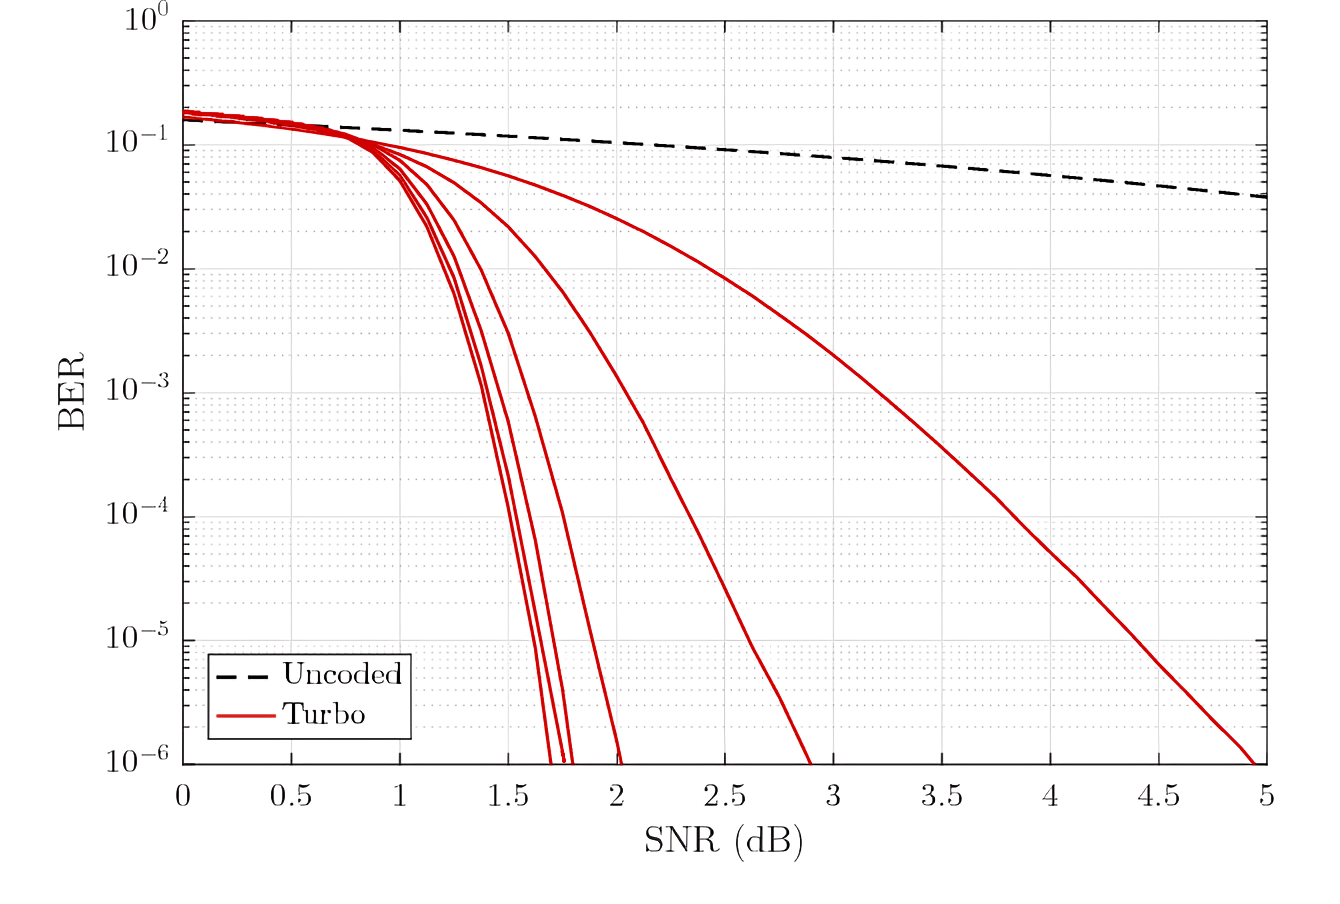
\includegraphics[width=0.5\textwidth]{imgs/turbo_code_ber.png}
\end{center}

In figura viene mostrata la convergenza con $K=2048$, $R=1/2$ e un numero di iterazioni, da sinistra a destra, pari rispettivamente a $32, 16, 8, 4, 2, 1$.


\section*{Space diversity}

In generale sia la frequency che time diversity richiedono parecchie risorse, per questo un altro tipo di diversity è spesso sfruttata, semplicemente utilizzando più antenne. Si possono sfruttare due tipologie di gain differenti:
\begin{itemize}
    \item \textbf{Array gain}: si tratta del guadagno di potenza ottenuto utilizzando più antenne rispetto all'utilizzo della singola antenna. Il guadagno è tanto più alto quanto è alta la correlazione spaziale del canale. Si sfruttano tipicamente antenne direzionali.
    \item \textbf{Diversity gain}: si tratta del guadagno ottenuto combinando i segnali ricevuti dalle varie antenne, considerati incorrelati. Tale guadagno è massimo quando i segnali sono completamente decorrelati. 
\end{itemize} 

Per assumere incorrelazione tra le varie antenne la loro distanza deve essere almeno la metà della lunghezza d'onda:
\[
    d_c = \frac{\lambda}{2} \quad \text{coherence distance}
\]  

La \textbf{coherence distance} deriva dalle proprietà di time varying del canale, tuttavia come si può osservare non ha dipendenze né dal tempo, né dalla velocità.

Le carrier frequencies attualmente utilizzate permettono di utilizzare anche antenne nel solito sistema sfruttando al massimo la space diversity. Bisogna comunque tenere in considerazione che ogni antenna ha bisogno della propria RF chain, quindi lo spazio occupato è maggiore rispetto alla grandezza dell'antenna.


\paragraph*{Canale MIMO (Multiple Input Multiple Output)}


Nei classici sistemi con un antenna in trasmissione ed un'antenna in ricezione, il canale, se narrow-band può essere descritto da uno scalare complesso.
Nel caso di sistemi con più antenne in trasmissione e ricezione tra ogni coppia di antenne vi è un canale differente, quindi l'intero sistema, per quanto riguarda il canale, può essere descritto tramite una mtrice complessa.
\[ 
    \mathbf{H} = 
    \begin{bmatrix}
        h_{11} & h_{12} & \ldots & h_{1M} \\
        h_{21} & h_{22} & \ldots & h_{2M} \\
        \vdots & \vdots & \ddots & \vdots \\
        h_{N1} & h_{N2} & \ldots & h_{NM} \\
    \end{bmatrix}
    , \quad
    \begin{array}{ll}
            \mathbf{H} \in \mathbb{C}^{N \times M} \\
            \mathbf{y} = \mathbf{Hx} 
    \end{array}
\]

Dove $\mathbf{x}$ è il segnale trasmesso, $\mathbf{y}$ è il segnale ricevuto e $\mathbf{H}$ è la matrice del canale. In questo caso, $M$ rappresenta il numero di antenne in trasmissione mentre $N$ il numero di antenne in ricezione.
\paragraph*{Canale SIMO (Single Input Multiple Output)}
\begin{center}
    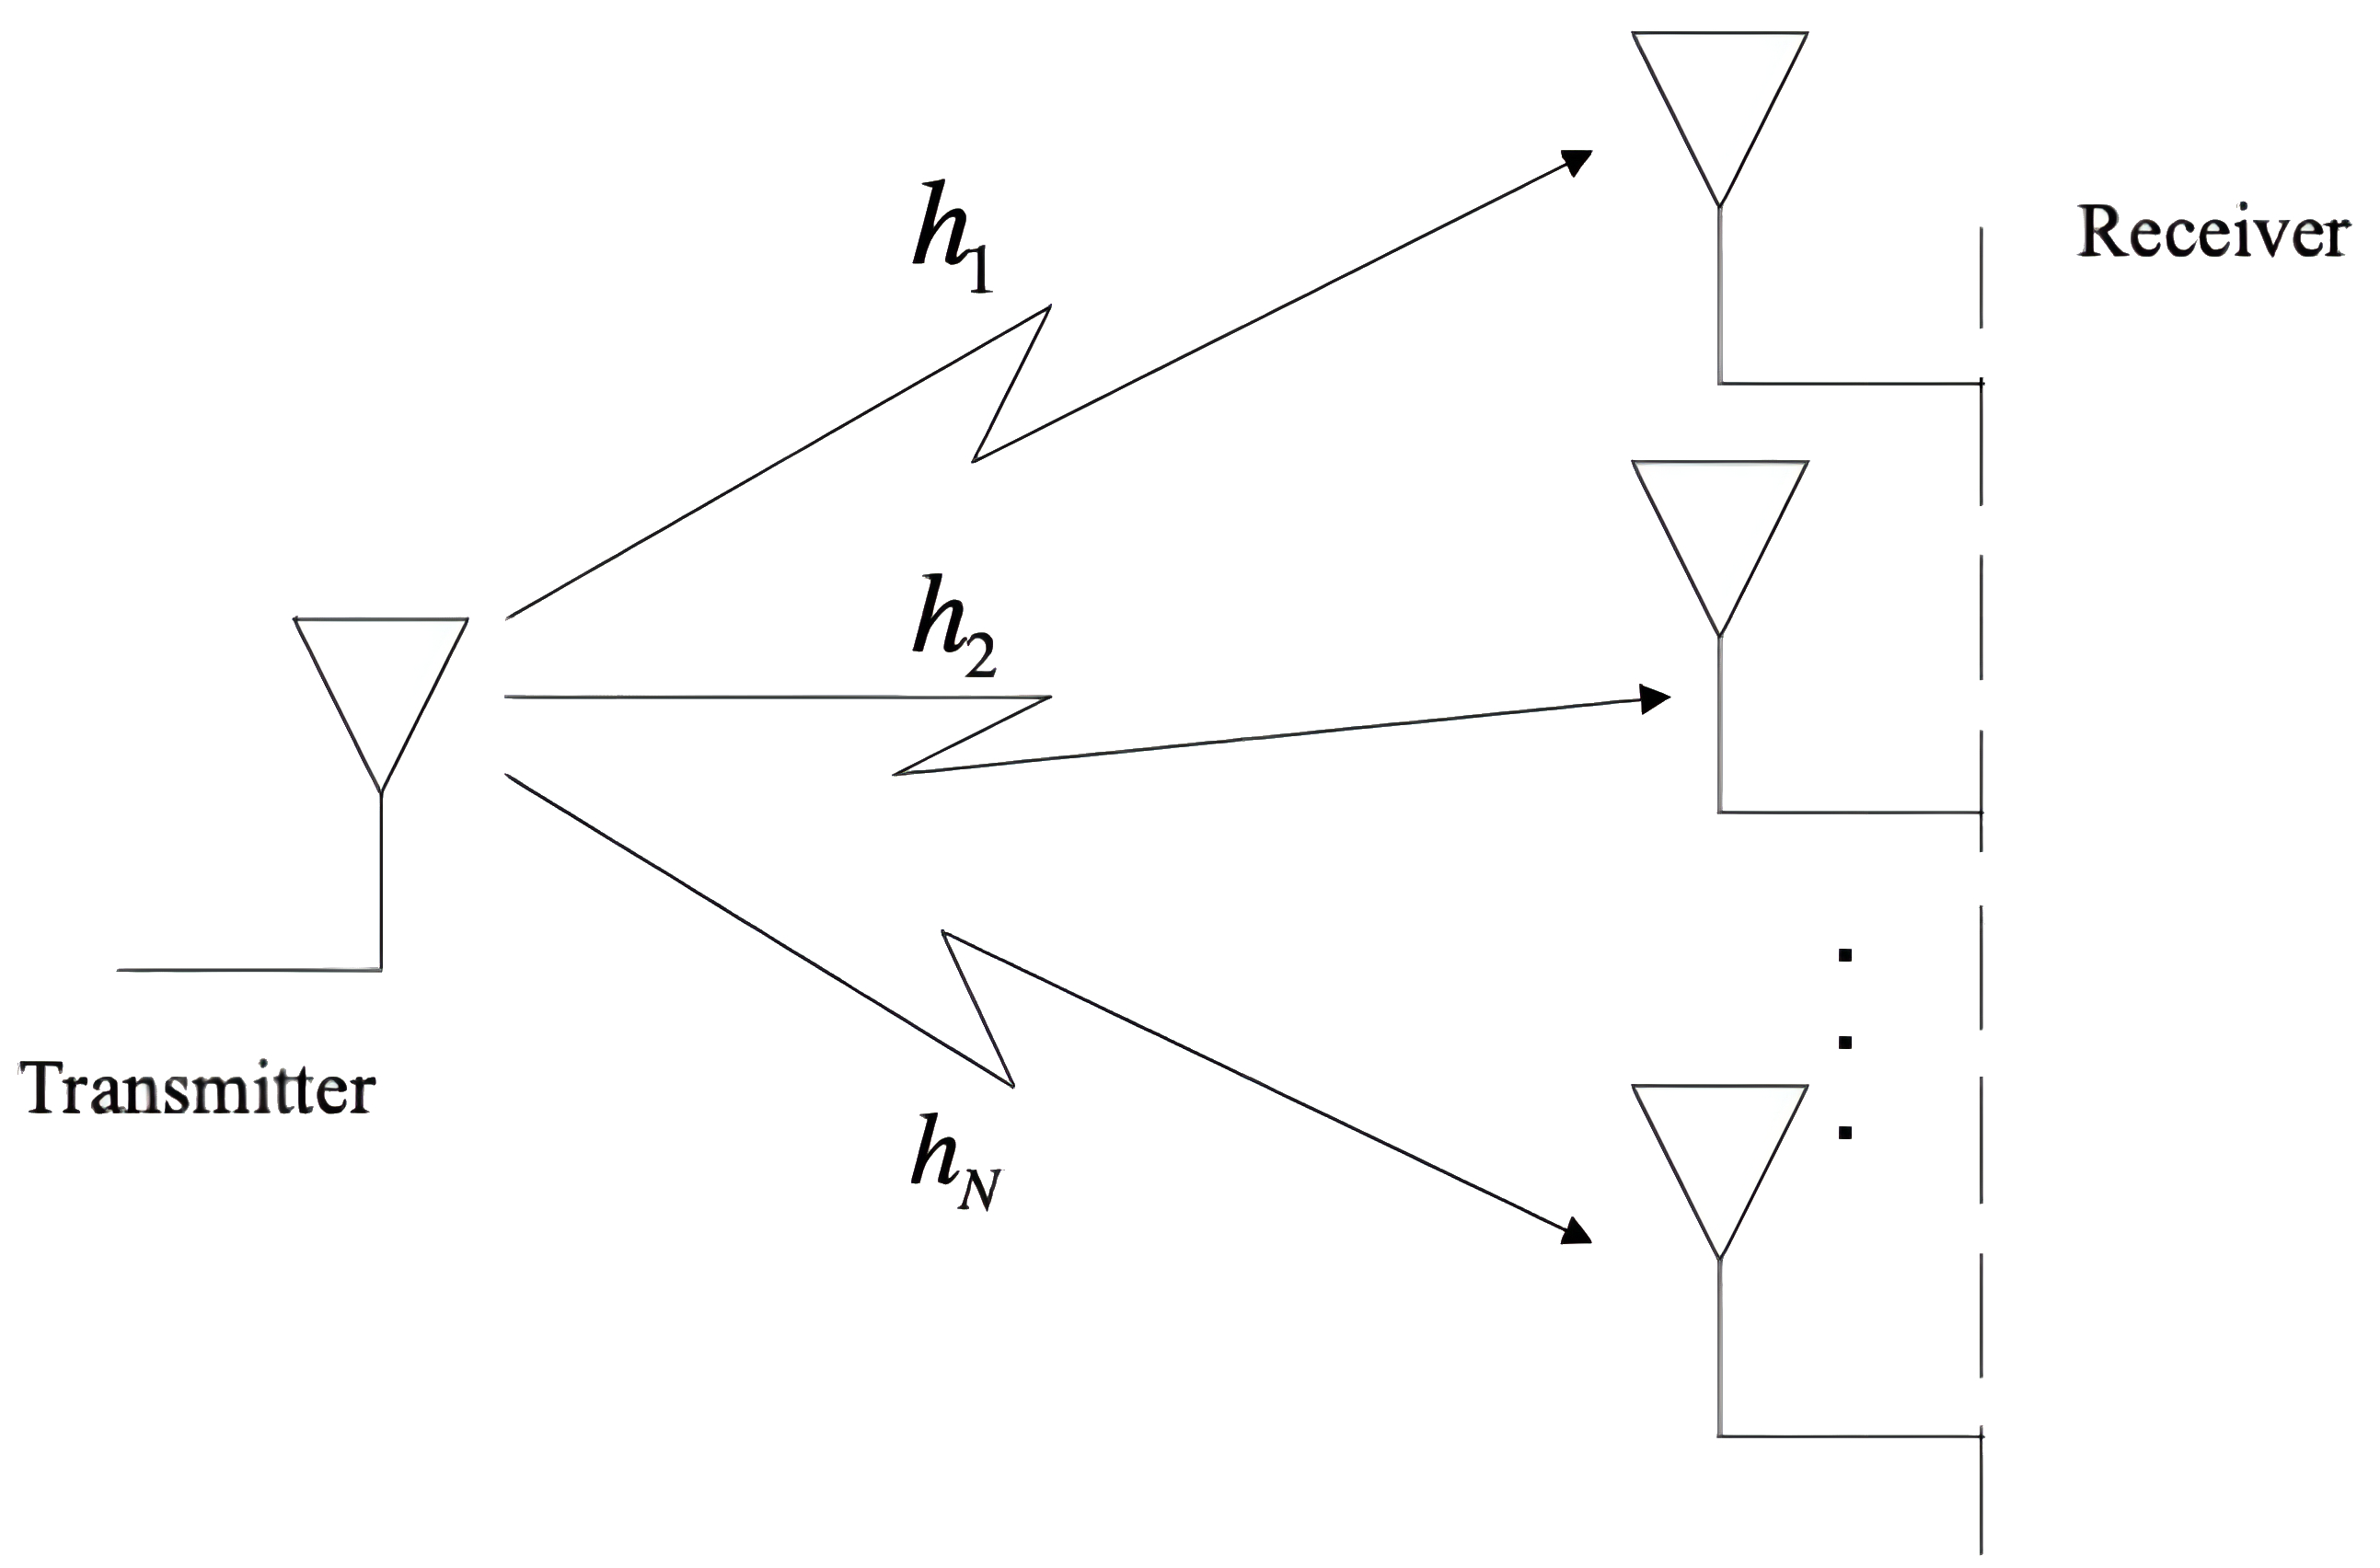
\includegraphics[width=0.4\textwidth]{imgs/simo.jpg}
\end{center}
Nel caso di unica antenna in trasmissione si parla di canale SIMO ed in tal caso $\mathbf{H} \in \mathbb{C}^{N \times 1}$
\[
    x_i[m] = h_i c_m + n_i[m] \quad i = 1, \ldots, N
\]
Questo rappresenta il segnale ricevuto sull'$i$-esima antenna.
È ragionevole assumere $h_i \in \mathbb{R}$ , dato che si può sempre moltiplicare $x_i[m]$ per $ e^{j\arg(h_i)} $ senza cambiare le statistiche del segnale.
Ogni segnale ha il proprio rumore e distorsione da parte del canale.

L'idea più semplice per sfruttare la diversity è scegliere di volta in volta il segnale con attenuzione minore, stimando il canale.
Tuttavia esistono tecniche in grado di utilizzare le informazioni provenienti da tutti i segnali ricevuti.
% TODO: i %w_i sono reali o complessi 
\[
    z[m] = \sum_{i=1}^{N} w_i x_i[m] = \sum_{i=1}^{N} w_i h_i c_m + \sum_{i=1}^{N} w_i n_i[m]
\]
dove $w_i$ sono i pesi assegnati alle varie antenne.


% TODO: ma anche qui si moltiplica per l'opposto della fase?
\[
    P = \mathbb{E} \left[ \left| \sum_{i=1}^{N} w_i h_i c_m  \right|^2 \right] = \mathbb{E} \left[  |c_m|^2  \right] \left| \sum_{i=1}^{N} w_i h_i \right|^2 =  A \left| \sum_{i=1}^{N} w_i h_i \right|^2
\]

\[
    \begin{array}{ll}
            P_N = \mathbb{E} \left[ \left| \sum_{i=1}^{N} w_i n_i[m]  \right|^2 \right] \\
            = \mathbb{E} \left[ \left( \sum_{i=1}^{N} w_i n_i[m] \right)  \left( \sum_{i=1}^{N} w_i n_i[m] \right)^*  \right] \\
            = \mathbb{E} \left[  \sum_{i=1}^{N} \sum_{j=1}^{N} w_i w_j^* n_i[m] n_j[m]^*  \right] \\
            = \sum_{i=1}^{N} \sum_{j=1}^{N} w_i w_j^* \mathbb{E} \left[ n_i[m] n_j[m]^* \right] \\
            = \sum_{i=1}^{N} \sum_{j=1}^{N} w_i w_j^* \sigma^2 \delta_{ij} \\
            = \sum_{i=1}^{N} w_i w_i^* \sigma^2 \\
            = \sum_{i=1}^{N} |w_i|^2 \sigma^2 \\
            = \sigma^2 \sum_{i=1}^{N} |w_i|^2 
    \end{array}
\]

% TODO: come si rimuovono i complessi?
L'obiettivo è massimizzare il SNR, che si può quindi scrivere come:
\[
    \text{SNR} = \frac{P}{P_N} = \frac{A}{\sigma^2} \frac{\left|\sum_{i=1}^{N} w_i h_i \right|^2}{\sum_{i=1}^{N} \left| w_i \right|^2} \leq \frac{A}{\sigma^2} \frac{\sum_{i=1}^{N} |w_i|^2 \sum_{i=1}^{N} \left| h_i \right|^2}{\sum_{i=1}^{N} |w_i|^2} = \frac{A}{\sigma^2} \sum_{i=1}^{N} |h_i|^2
\]

dove la disuguaglianza è dovuta alla disuguaglianza di Schwarz. Imponendo la condizione $w_i = h_i^*$ si ottiene il massimo SNR possibile e quindi vale l'uguaglianza:
\[ 
    \text{SNR} = \frac{A}{\sigma^2} \frac{\left(\sum_{i=1}^{N} \left| h_i \right|^2 \right)^2}{\sum_{i=1}^{N} \left| h_i^2 \right|} = \frac{A}{\sigma^2} \sum_{i=1}^{N} |h_i|^2
\]


% TODO: h è complesso? Nel caso vi vuole il modulo?
Se si ha un unico canale l'espressione del SNR si riduce al semplice rapporto $\frac{A}{\sigma^2}h$, ovvero la forma valida per un semplice fading channel.
\paragraph*{MISO (Multiple Input Single Output)}
\begin{center}
    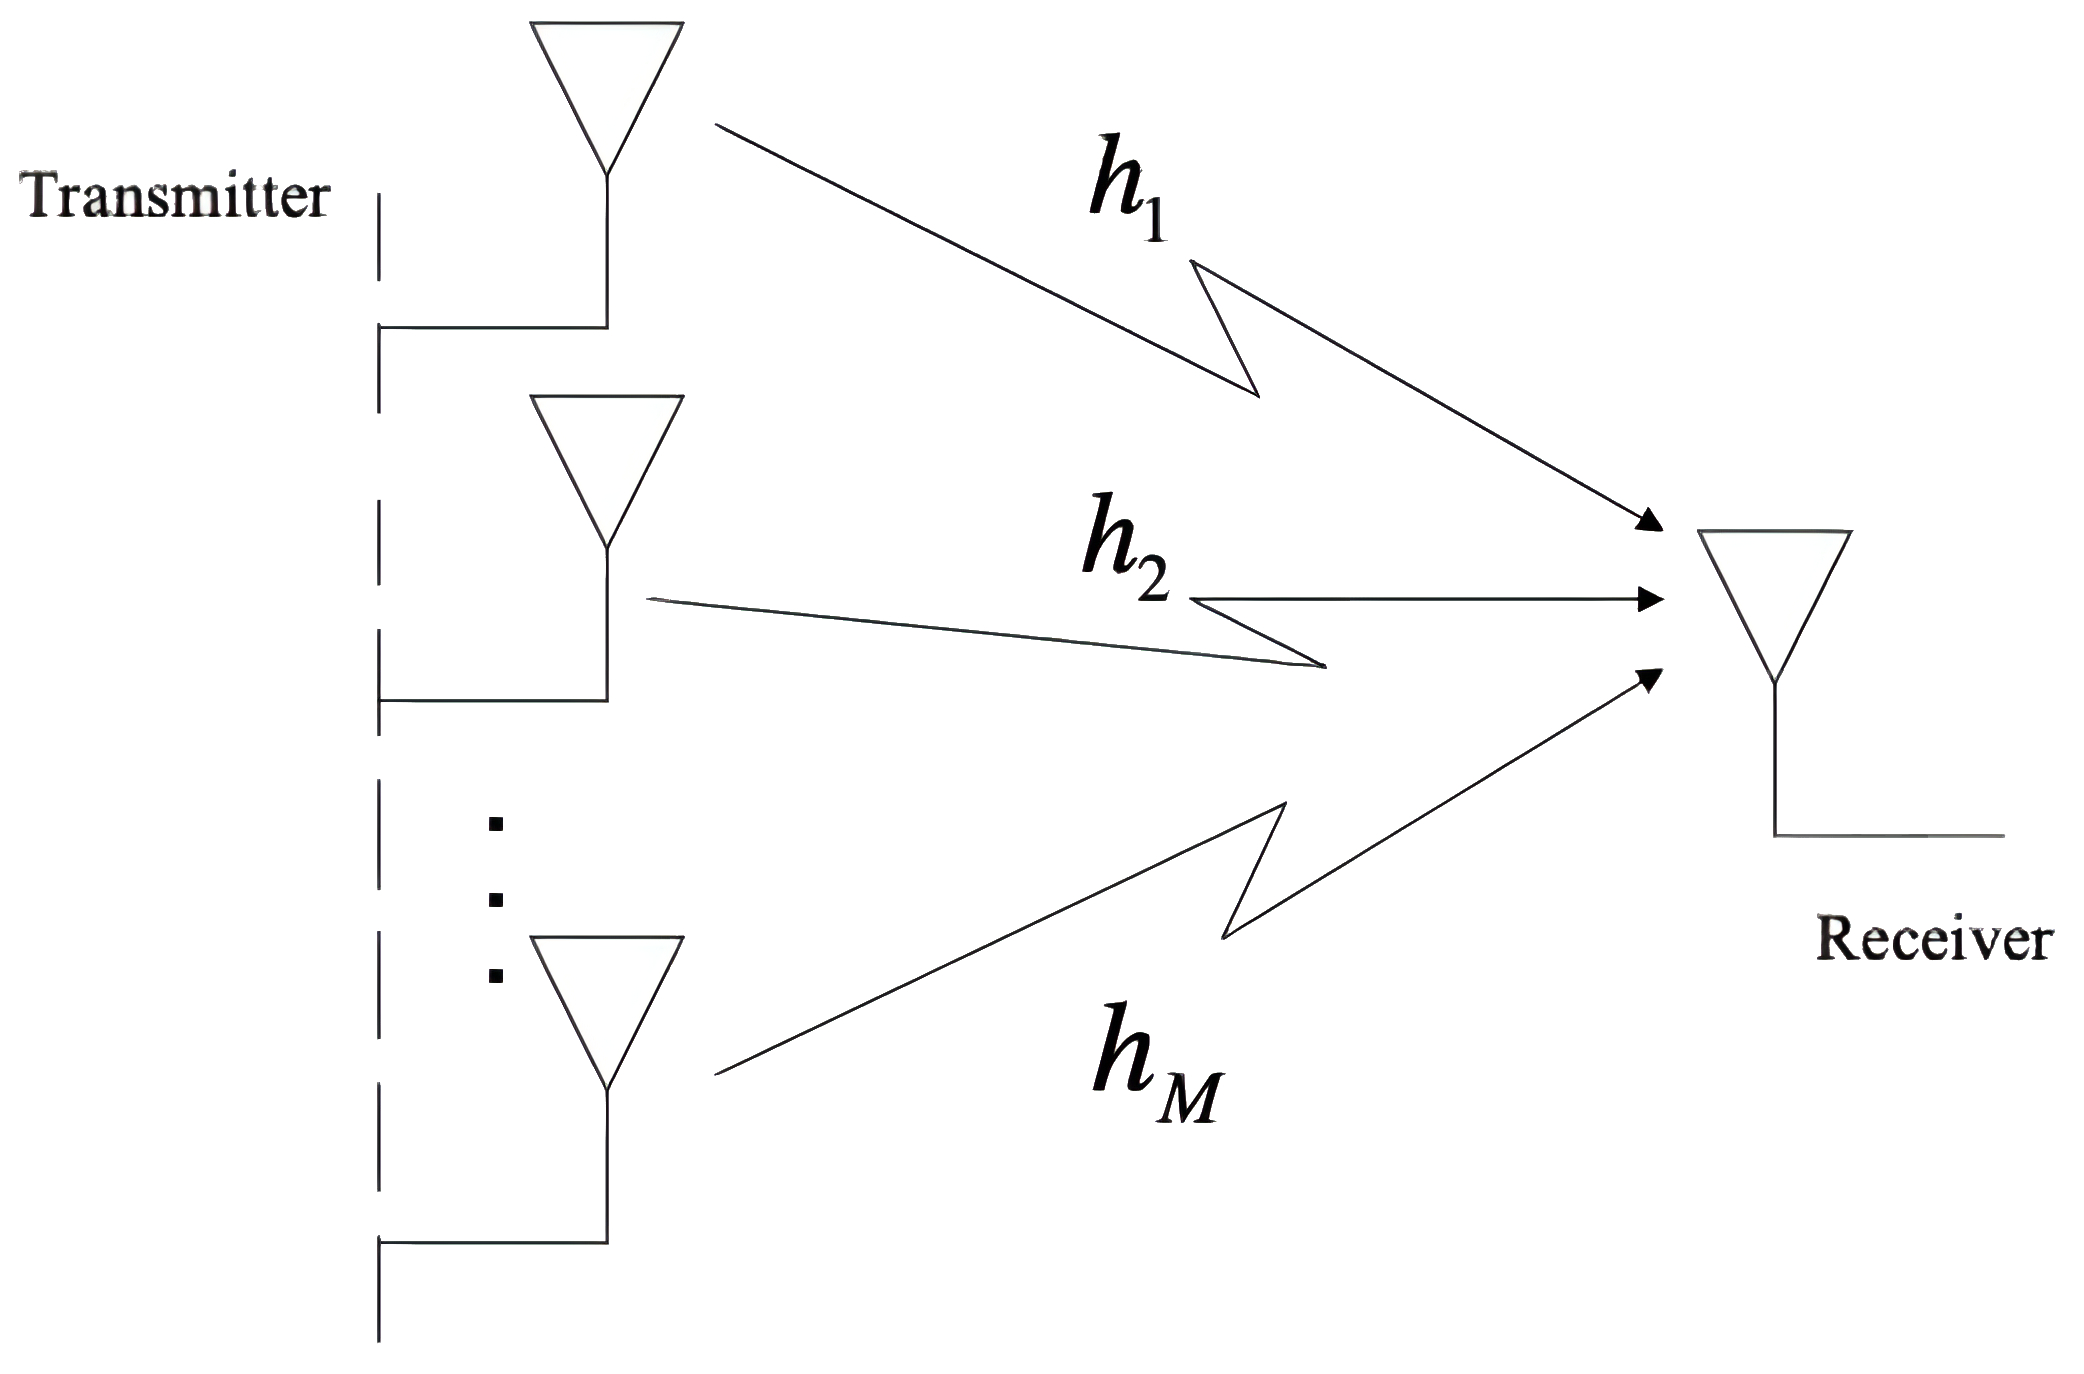
\includegraphics[width=0.4\textwidth]{imgs/miso.jpg}
\end{center}
Per quanto riguarda la configurazione con più antenne in trasmissione e singola antenna in ricezione, sistema MISO, si ottiene la stessa espressione con alcuni accorgimenti lato trasmettitore
\[
    x[m] = \sum_{i=1}^{N} h_i y_i[m] + n[m] \quad \text{segnale ricevuto tramite l'unica antenna disponibile}
\]

La differenza sostanziale con il caso SIMO è che i vari segnali sono combinati ``naturalmente" durante la trasmissione e ricevuti quindi già aggregati. 
La scelta dei coefficienti non può essere effettuata lato ricevitore, ma deve essere il trasmettitore a scegliere stimando il canale, lato ricevitore la stima è ovviamente più complessa rispetto a quella che effettuerebbe il ricevitore per proprio conto.
L'operazione effettuata dal trasmettitore è detta \textbf{spatial precoding} ed il simbolo è denominato \textbf{spatial pre-coded symbol}.
\[
    y_i[m] = b_i c_m \quad \text{simbolo trasmesso sulla $i$-esima antenna}
\]
L'energia spesa dipende anche dal coefficiente $b_i$, l'obiettivo è comunque utilizzare la solita energia usata nel caso di singola antenna.

Il rapporto SNR è massimizzato scegliendo $b_i = \frac{h_i^*}{ \| \mathbf{h} \| }$

\[
    x[m] = \sum_{i=1}^{N} h_i y_i[m]  = \sum_{i=1}^{N} h_i b_i c_m + n[m] = \sum_{i=1}^{N} \frac{h_i h_i^*}{\| \mathbf{h} \|} c_m + n[m] = \| \mathbf{h} \| c_m + n[m]
\]
\[
    P = \|\mathbf{h} \|^2 \ \mathbb{E} \left[\left| c_m \right|^2 \right] = \|\mathbf{h} \|^2  A
\]
\[
    P_N = \sigma^2  
\]
\[
    \text{SNR} = \frac{P}{P_N} = \sum_{i=1}^{N} |h_i|^2 \frac{A}{\sigma^2}    
\]

La differenza tra il caso con singola antenna (sia lato trasmettitore che ricevitore) e il caso con più antenne (MISO/SIMO) è dato dal fattore $\| \mathbf{h} \| = \sum_{i=1}^{N} |h_i|^2$.
Considerando i guadagni del canale come variabili aleatore con distribuzione di Rayleigh è possibile calcolare la distribuzione della somma come convoluzione delle PDF.
\[
    f_{\| \mathbf{h} \|^2} (x) = \frac{1}{D-1} x^{D-1} e^{-x}
\]
Il risultato dipende dal nnumero di antenne, tuttavia in generale si ottiene un \textbf{array gain}, ovvero uno spostamente del valor medio dei gain verso destra (più potenza).
Inoltre il \textbf{diversity gain} si manifesta riducendo notevolmente la probabilità di ottenere guadagni molto bassi.
Ciò è visibile confrontando gli integrali delle due PDF.

\paragraph*{MIMO (Multiple Input Multiple Output)}

Il caso generale MIMO, ovvero con più antenne sia in trasmissione che ricezione, sfrutta una tecnica denominata \textbf{spatial multiplexing} ed è basata sulla decomposizione ai valori singolari (SVD) della matrice $\mathbf{H}$ che descrive il canale.

\paragraph*{SVD (Singular Value Decomposition)}

Data una matrice $\mathbf{A} \in \mathbb{C}^{m \times n}$, con  $p = \text{rank} (\mathbf{A})$, la SVD permette di scrivere la matrice come prodotto di tre matrici:
\[
    \mathbf{A} = \mathbf{U} \mathbf{\Sigma} \mathbf{V}^H
\]
con $\mathbf{U} \in \mathbb{C}^{m \times p}$, $\mathbf{\Sigma} \in \mathbb{C}^{p \times p}$ e $\mathbf{V} \in \mathbb{C}^{n \times p}$,
dove $\mathbf{U}$ e $\mathbf{V}$ sono matrici unitarie, mentre $\mathbf{\Sigma} = diag(\sigma_1, \ldots, \sigma_p)$ è una matrice diagonale con $\sigma_1 \geq \sigma_2 \geq \ldots \geq \sigma_p$. In un sistema MIMO, se il canale è sufficientemente multipath, la matrice $\mathbf{H}$ ha rango pieno, dunque:
\[
    p = \text{rank}(H) = \min(N_R, N_T)
\]

La tecnica di \textbf{spatial multiplexing} consiste nell'effettuare sia un pre-coding lato trasmettitore, sia un combining lato ricevitore, dunque utilizzando due pesi differenti. In questo modo è possibile creare un certo numero di canali ortogonali indipendenti, detti \textbf{spatial channels}.
\[
    \begin{array}{ll}
        \mathbf{H} = \mathbf{U} \mathbf{\Sigma} \mathbf{V}^H \quad \text{decomposizione SVD matrice del canale MIMO} \\
        \mathbf{B} = \mathbf{V} \quad \text{matrice pre-coder (Tx)} \\
        \mathbf{W} = \mathbf{U} \quad \text{matrice combiner (Rx)}
    \end{array}
\]
\begin{center}
    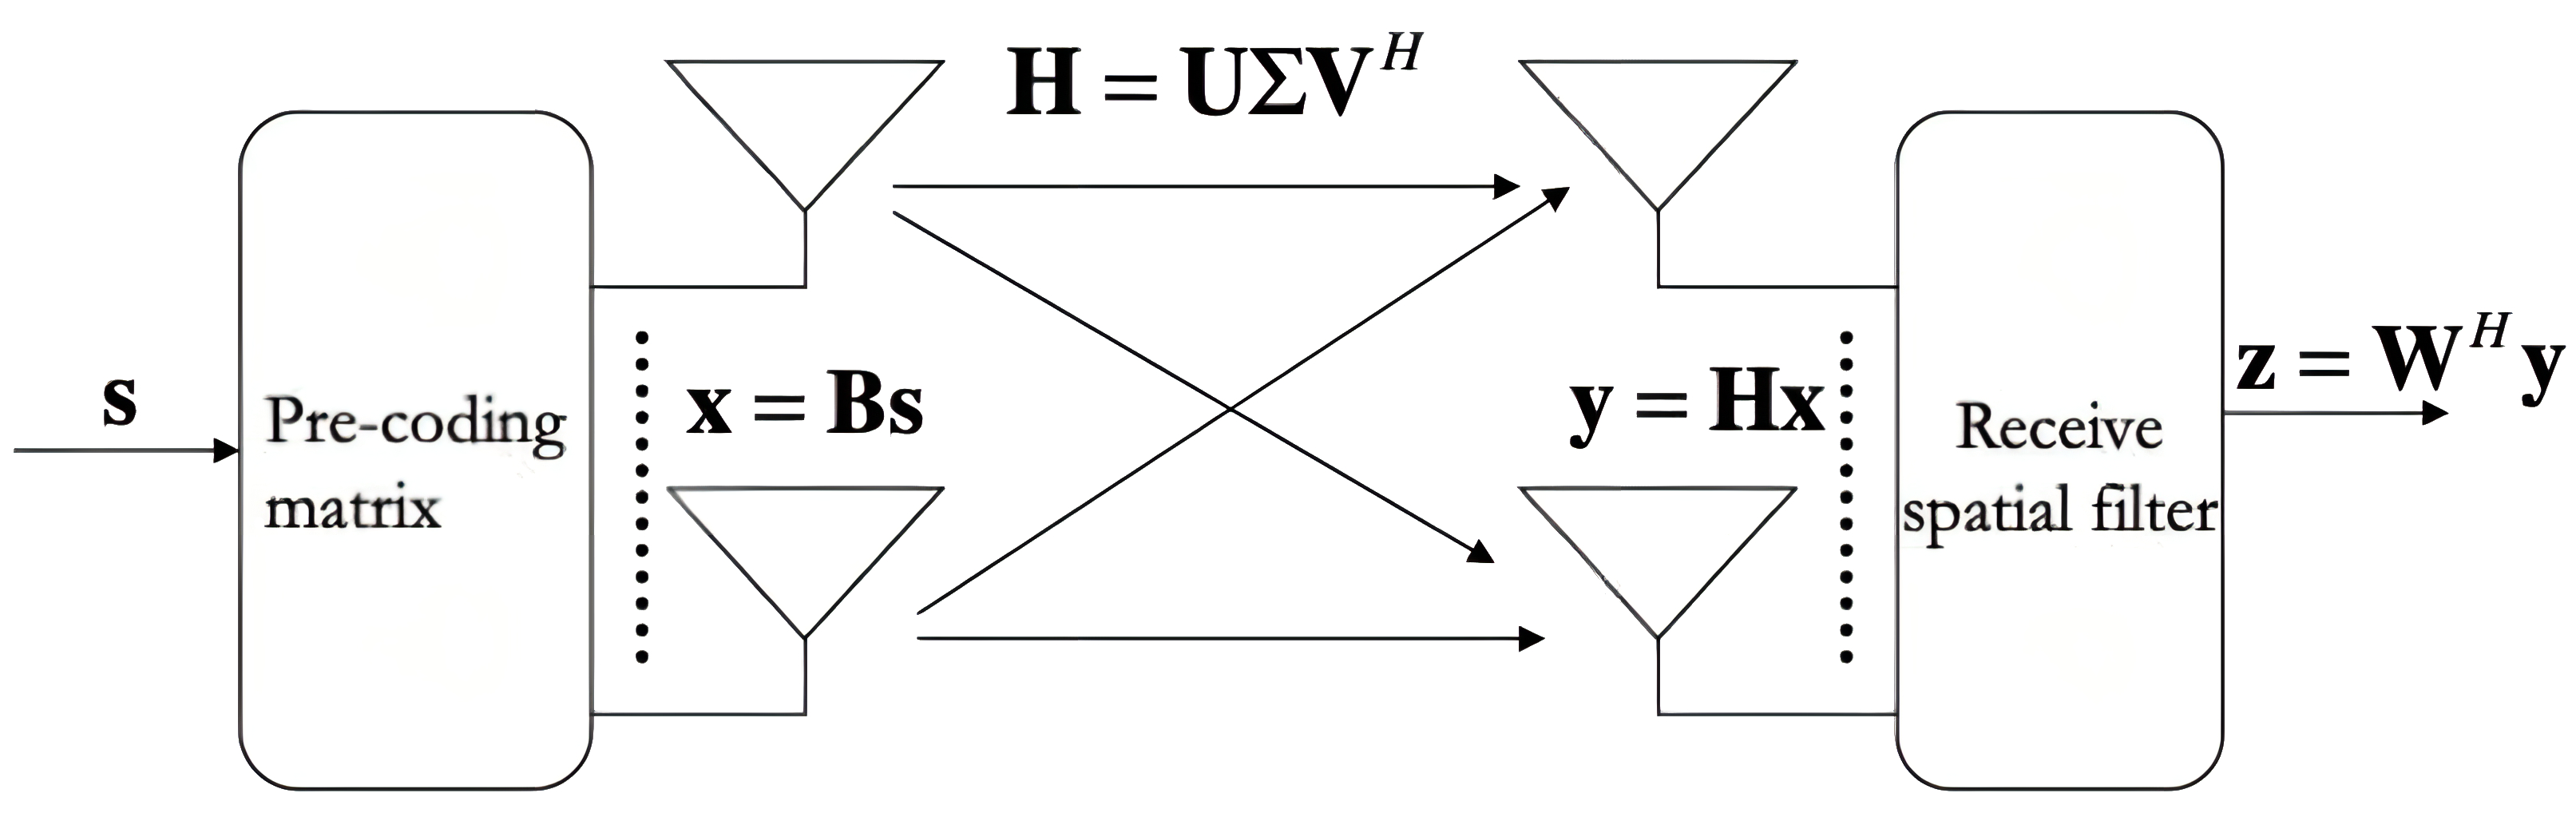
\includegraphics[width=0.8\textwidth]{imgs/mimo.jpg}
\end{center}

Scegliendo in questo modo le matrici si ottiene:
\[
    \begin{array}{ll}
        \mathbf{z} = \mathbf{W}^H \mathbf{y}  \\
        = \mathbf{W}^H \left( \mathbf{H} \mathbf{x} + \mathbf{n}  \right) \\  
        = \mathbf{W}^H \left( \mathbf{H} \mathbf{B} \mathbf{s} + \mathbf{n} \right) \\
        = \mathbf{W}^H \mathbf{H} \mathbf{B} \mathbf{s} + \mathbf{W}^H \mathbf{n}  \\
        = \mathbf{U}^H \mathbf{H} \mathbf{V} \mathbf{s} + \mathbf{W}^H \mathbf{n} \\
        = \mathbf{\Sigma} \mathbf{s} + \mathbf{W}^H \mathbf{n}
    \end{array}
\]
Sebbene ogni antenna riceva dei segnali sovrapposti, scegliendo le matrici in questa maniera è possibile ottenere dei canali ortogonali che non interferiscono tra loro dato che la matrice $\mathbf{\Sigma}$ è diagonale.

Considerando un sistema $2 \times 2$ per esempio si ottiene:
\[
    \begin{cases*}
        y_1 = h_{11} x_1 + h_{12} x_2 + n_1 \\
        y_2 = h_{21} x_1 + h_{22} x_2 + n_2
    \end{cases*}
    \quad
    \text{segnali sovrapposti su ogni antenna}
\]

L'utilizzo di un canale MIMO può incrementare la capacità del sistema, tuttavia è necessario tenere in considerazione anche i valori singolari, i quali potrebbero comportare un'attenuazione eccessiva.


\[
    \mathbf{z} = \begin{matrix}
        \begin{bmatrix}
            \sigma_1 s_1 + n_1' \\
            \sigma_2 s_2 + n_2'
        \end{bmatrix}
    \end{matrix}
    \quad 
    \text{segnale ottenuto dopo combining lato ricevitore, non c'è alcuna sovrapposizione}
\]


% TODO: aggiungere considerazioni sull'aumento della capacità del sistema


\section*{Frequency diversity}

La formula di Shannon fornisce il massimo rate sostenibile su un dato canale di trasmissione:
\[
    C = B \log_2 \left( 1 + \text{SNR} \right), \quad \text{SNR} = \frac{\left| H \right|^2 P}{\sigma^2}
\]
Dove $H$ è il guadagno del canale.
In sistemi reali ci si può solo avvicinare al limite teorico e vi è una forte dipendenza, per quanto riguarda l'efficienza spettrale, del coding rate e modulation order, data dalla dimensione della costellazione di simboli per cui esiste un trade-off tra capacità di trasmissione ed energia richiesta.
In particolare $\log_2 \left( 1 + \text{SNR} \right)$ è l'efficienza spettrale.
Il rate di trasmissione reale può essere approssimato:
\[
    R_b = \log_2 M \  R \frac{1}{T}  \approx m R B
\]

Dove è $M$ è il numeri di simboli nella costenllazione, $R$ è il coding rate \footnote{con $R_s$ indichiamo il symbol rate, ovvero $\frac{1}{T}$, mentre con $R$ il symbol rate} e $T$ è il symbol time, si fa l'approssimazione che $\frac{1}{T} \approx B$. 


Per rispettare il limite di capacità si deve avere:
\[
    m R B < C \quad \Rightarrow \quad m R < \log_2 (1 + \text{SNR})
\]
Misurando il SNR è possibile adattare i valori di $m$ ed $R$, ad esempio in base alla posizone in una cella.
I valori di $m$ ed $R$ che si possono utilizzare appartengono ad un insieme finito, non è possibile scegliere arbitrariamente.

\begin{table}[H]
    \resizebox{\textwidth}{!}{
        \centering
        \begin{tabular}{|c|l|c|c|c|}
        \hline
        \textbf{Radio Bearer Index} & \textbf{Name} & \textbf{Modulation} & \textbf{Channel Coding Rate} & \textbf{Bearer Efficiency} ($\log_2(1+\text{SNR})$, bits/symbol) \\ \hline
            1  & QPSK 1/12 & QPSK & 0.0761719 & 0.1523 \\ \hline
            2  & QPSK 1/9  & QPSK & 0.117188  & 0.2344 \\ \hline
            3  & QPSK 1/6  & QPSK & 0.188477  & 0.377  \\ \hline
            4  & QPSK 1/3  & QPSK & 0.300781  & 0.6016 \\ \hline
            5  & QPSK 1/2  & QPSK & 0.438477  & 0.877  \\ \hline
            6  & QPSK 3/5  & QPSK & 0.587891  & 1.1758 \\ \hline
            7  & 16QAM 1/3 & 16QAM & 0.369141  & 1.4766 \\ \hline
            8  & 16QAM 1/2 & 16QAM & 0.478516  & 1.9141 \\ \hline
            9  & 16QAM 3/5 & 16QAM & 0.601563  & 2.4063 \\ \hline
            10 & 64QAM 1/2 & 64QAM & 0.455078  & 2.7305 \\ \hline
            11 & 64QAM 1/2 & 64QAM & 0.553711  & 3.3223 \\ \hline
            12 & 64QAM 3/5 & 64QAM & 0.650391  & 3.9023 \\ \hline
            13 & 64QAM 3/4 & 64QAM & 0.753906  & 4.5234 \\ \hline
            14 & 64QAM 5/6 & 64QAM & 0.852539  & 5.1152 \\ \hline
            15 & 64QAM 11/12 & 64QAM & 0.925781  & 5.5547 \\ \hline
        \end{tabular}
    }
\end{table}

Come si evince dala tabella, in pratica c'è un mapping diretto tra SNR misurato (channel quality indicator, CQI) e lo specifico ordine di modulazione e coding rate di una trasmissione.
La qualità del canale in termini di SNR può essere espressa tramite \textbf{radio beared index} ($\in [1, 15]$).
Utilizzando la modulazione OFDM l'idea sarebbe adattare $m$ ed $R$ per ogni canale, distribuendo la potenza nel modo più efficace possibile per massimizzare il rate di trasmmissione. Questo problema è inidcato con il termine di \textbf{water-filling}, la potenza a disposizione è invece detta \textbf{power budget}. Nella pratica si tratta di un problema di ottimizzazione per il quale sono definiti alcuni vincoli da rispettare:

% TODO: p non lo metterei, perché non è chiaro cosa rappresenti
\[
    \begin{cases}
       \underset{\mathbf{p}}{\text{max}} \sum_{n=1}^{N} \log_2(1 + \frac{P_n}{\sigma_n^2}), \quad P_n \geq 0 \quad n = 1, \ldots, N \\
       \sum_{n=1}^{N} P_n = P_0 \quad \text{(power budget)} \\
        P_n \geq 0 \quad n = 1, \ldots, N
    \end{cases}    
\]

Dove $\sigma_n^2 = \frac{\sigma^2}{\left| \mathbf{H}_{n, n} \right| ^2}$. Il termine $B$ non appare nell'espressione in quanto costante per ogni canale, massimizzare il rate o l'efficienza spettrale genera lo stesso risultato.

La lagrangiana del problema è:
\[
    \mathcal{L}(P_1, \hdots, P_N, \lambda ) = \sum_{n=1}^{N} \log_2(1 + \frac{P_n}{\sigma_n^2}) - \lambda \left( \sum_{n=1}^{N} P_n - P_0 \right)
\]
La derivata rispetto a $P_n$ posta a 0 per la condizione di stazionarietà è:
\[
    \frac{\partial \mathcal{L}}{\partial P_n} = \frac{1}{\ln(2)} \frac{1}{1 + \frac{P_n}{\sigma_n^2}} \frac{1}{\sigma_n^2} - \lambda = 0, \quad n = 1, \ldots, N
\]
overro il gradiente:
\[
    \nabla_{P_1, \hdots, P_N} \mathcal{L} = \begin{bmatrix}
        \frac{1}{\ln(2)} \frac{1}{1 + \frac{P_1}{\sigma_1^2}} \frac{1}{\sigma_1^2} - \lambda \\
        \frac{1}{\ln(2)} \frac{1}{1 + \frac{P_2}{\sigma_2^2}} \frac{1}{\sigma_2^2} - \lambda \\
        \vdots \\
        \frac{1}{\ln(2)} \frac{1}{1 + \frac{P_N}{\sigma_N^2}} \frac{1}{\sigma_N^2} - \lambda \\
\end{bmatrix} = \mathbf{0}
\]

La soluzione del problema è:
\[
    \hat{P}_n = \frac{1}{\lambda \ln(2)} - \sigma_n^2, \quad n = 1, \ldots, N
\]
considerando il vincolo che $P_n \geq 0$ e ponendo $\mu = \frac{1}{\lambda \ln(2)}$ si ottiene:
\[
    \hat{P}_n = \text{max} \{ 0, \mu - \sigma_n^2    \} = (\mu - \sigma_n^2)^+, \quad n = 1, \ldots, N
\]

Per ottenere dei valori è necessario calcolare $\mu$, scelto in modo da rispettare il vincolo sulla potenza a disposizione.
\[
    \sum_{n=1}^{N} (\mu - \sigma_n^2)^+ = P_0
\]
\[
    \begin{cases}
        f(\mu) = \sum_{n=1}^{N} (\mu - \sigma_n^2)^+ - P_0 \\
        f: \mathbb{R}^n \rightarrow \mathbb{R}
    \end{cases}
\]
La risoluzione dell'equazione garantisce il valore $\mu$ tale per cui i vincoli sono rispettati, è quindi necessario trovare lo zero di una funzione in $\mu$, ad esempio con il metodo della bisettrice.
Il metodo dei bisezione può essere applicato dato che la funzione risulta continua e monotona su% TODOl dominio.
Il termine water-filling deriva dal fatto che osservando il grafico della distribuzione della potenza, si ha l'impressione che la potenza si distribuisca come l'acqua all'interno di un contenitore con superiore irregolare, fino ad un livello pari a $\mu$.
La distribuzione è ottima e rappresenta la miglior situazione per sfruttare la frequency diversity del canale.
In sostanza la distribuzione favorisce i canali con miglior qualità, scartando completamente quelli la cui capacità è troppo bassa.



% TODO: aggiungere qualcosa sul waterfilling


% TODO: la fft size è 2048 come il numero di subcarriers?

La banda di un singolo subcarrier è calcolata come:
\[
    \Delta f = \frac{f_s}{N} = \frac{30.72 \text{ MHz}}{2048} = 15 \text{ kHz}
\]
La banda di un resource block (RB), cioè la minima unità allocabile, è calcolata come:
\[
    B_{RB} = 12 \times 15 \text{ kHz} = 180 \text{ kHz}
\]
La raw bandwidth è calcolata come:
\[
B_{raw} = 1200 \times 15 \text{ kHz} = 18 \text{ MHz}
\]
La disponibilità di banda è calcolata togliendo dalla banda grezza la banda usata per informazioni di sincronizzazione e controllo:
\[
B_{av} = B_{raw} - 4 \text{ MHz} = 14 \text{ MHz}
\]
Il rate massimo per un canale SISO è:
\[
    R_{1 \times 1} = 0.9258 \times 8 \times 14 \text{ MHz} \approx 100 \text{ Mb/s}
\]
Con il carrier aggregation: quando gli operatori comprano lo spettro di trasmissione, compratno chunks dello spettro che sono più larghi di 20 MHz, e possono essere aggreagati per un singolo utente
Con un canale MIMO $4 \times 4$ si ha un massimo data rate di:
\[
    R_{4 \times 4} = 4 \times 0.9258 \times 8 \times 14 \text{ MHz} \approx 400 \text{ Mb/s}
\]


I terminali più avanzati possono aggregare più bande da 20 MHz ciascuna, per esempio 3 con $4 \times 4$ MIMO e 2 con $2 \times 2$ MIMO, ottenendo un rate di:
\[
    R_{\text{aggregated}} = 3 \times 400 \text{ Mb/s} + 2 \times 200 \text{ Mb/s} = 1.6 \text{ Gb/s}
\]


\section*{LTE (Long Term Evolution)}


\begin{center}
    \begin{threeparttable}
        \begin{tabular}{|l|l|} 
            \hline
            \textbf{Parametro} & \textbf{Valore} \\
            \hline
             Frequenza di campionamento\tnote{1 } \  ($f_s$) & 30.72 MHz \\
            \hline
            Subcarrier disponibili (Dimensione FFT, $N$) & 2048 \\
            \hline
            Subcarrier utilizzati & 1200 \\
            \hline
            Subcarrier di guardia\tnote{2} \ di livello 0 & 848 \\
            \hline
            Subcarrier per blocco risorsa (RB) & 12 \\
            \hline
            Tasso di codifica ($R$) & $[0.0762, 0.9258]$ \\
            \hline
            Ordine di modulazione ($M$) & 256 (8 bit/simbolo) \\
            \hline
            Numero blocchi OFDM per slot & 7 \\
            \hline
            Durata dello slot & 0.5 ms \\
            \hline
        \end{tabular}
        \begin{tablenotes}
            \item[1] Per OFDM il tempo di campionamento è $T_s = \frac{1}{B}$.
            \item[2] Subcarrier non utilizzati per evitare interferenze.
        \end{tablenotes}
    \end{threeparttable}
\end{center}
Lo standard LTE è il primo ad adottare una modulazione OFDM, con i seguenti parametri:
\[
    \begin{array}{ll}
        f_s = \frac{1}{T_s} = 30.72 \text{ MHz} & \text{(banda totale/sampling frequency, in OFDM $T_s=\frac{1}{B}$)} \\
        N = 2048 & \text{(numero di subcarrier disponibili)} \\
        \Delta f = \frac{f_s}{N} = 15 \text{ kHz} & \text{(banda di un singolo subcarrier)} \\
    \end{array}    
\]
L'allocazione delle risorse di banda agli utenti è indicata come OFDMA, ovvero FDMA basata su OFDM, per cui la banda assegnata è un multiplo intero della banda di un canale.
L'allocazione minima per ciascun utente è un blocco, composto da 12 subcarrier, chiamato \textbf{Resource Block} (RB), che quindi occupa $12 \times 15 \text{ kHz} = 180 \text{ kHz}$.
Inoltre l'allocazione delle risorse richiede anche l'assegnamente di slot temporali, ovvero il tempo entro cui i blocchi di banda sono utilizzabili.
L'unità minima è un slot composta da 7 blocchi OFDM (simboli) della durata di 0.5 ms.
\begin{itemize}
    \item slot temporale: 0.5 ms (7 simboli OFDM) 
    \item blocco di banda: 180 kHz (12 subcarrier)
\end{itemize}
Delle 2048 subcarrier solo 1200 sono utilizzate, le altre rappresentano virtual subcarrier. Per cui:
\[
    B_{\text{raw}} = 1200 \times 15 \text{ kHz} = 18 \text{ MHz}  
\]
Sebbene possa sembrare un numero molto alto di frequenze non utilizzate, la scelta deriva dall'utilizzo di un $f_s$ molto alto, tuttavia lo spettro realmente occupato è circa 20 MHz.
Inoltre un'altra porzione di spettro è utilizzata per informazioni di controllo e sincronizzazione, riducendo la banda disponibile di 4 MHz.
\[
    B_{\text{av}} = B_{\text{raw}} - 4 \text{ MHz} = 1200 \cdot 15 \text{ kHz} - 4 \text{ MHz} = 14 \text{ MHz}
\]

Per quanto riguarda il coding rate e modulation order la scelta avvviene in base alla qualità del link, valutata in termini di CQI (Channel Quality Indicator). Le modulazioni possibili sono quelle comprese tra 4-QAM e 256-QAM, mentre il range di coding rate varia da 0.0762 a 0.9258.
Il massimo rate su un canale SISO può quindi essere calcolato:
\[
    R_{1 \times 1} = 0.9258 \cdot 8 \cdot 14 \text{ MHz} \approx 100 \text{ Mbps}
\]
Lo standard prevedere il supporto per canali MIMO in diverse configurazioni, fino a 4$\times$4, per cui si ottiene un rate potenzialmente quadruplicato:
\[
    R_{4 \times 4} = 4 \cdot R_{1 \times 1} = 400 \text{ Mbps}
\]
I terminali avanzati possono combinare più bande di 20 MHz per raggiungere velocità fino a 2 Gbps.
Tuttavia, in pratica è difficile ottenere tali velocità poiché richiederebbero condizioni ottimali del canale, vicinanza alle antenne, e l'allocazione di tutte le risorse a un solo utente.
Inoltre, gli operatori di solito impongono limiti alle prestazioni massime. 
Con il carrier aggregation, gli operatori acquistano blocchi di spettro più larghi di 20 MHz che possono essere aggregati per aumentare la banda disponibile per un singolo utente, per esempio 3 con $4 \times 4$ MIMO e 2 con $2 \times 2$ MIMO, ottenendo un rate di:
\[
    R_{\text{aggregated}} = 3 \times 400 \text{ Mb/s} + 2 \times 200 \text{ Mb/s} = 1.6 \text{ Gb/s}
\]



\end{document}



